%; whizzy paragraph
%; whizzy-paragraph "^\\\\dancersection"
% -initex iniptex -latex platex -format platex -bibtex jbibtex -fmt fmt
% 以上 whizzytex を使用する場合の設定。

%     Tokyo Debian Meeting resources
%     Kansai Debian Meeting resources
%     Copyright (C) 2008 Junichi Uekawa
%     Copyright (C) 2008 Nobuhiro Iwamatsu

%     This program is free software; you can redistribute it and/or modify
%     it under the terms of the GNU General Public License as published by
%     the Free Software Foundation; either version 2 of the License, or
%     (at your option) any later version.

%     This program is distributed in the hope that it will be useful,
%     but WITHOUT ANY WARRANTY; without even the implied warranty of
%     MERCHANTABILITY or FITNESS FOR A PARTICULAR PURPOSE.  See the
%     GNU General Public License for more details.

%     You should have received a copy of the GNU General Public License
%     along with this program; if not, write to the Free Software
%     Foundation, Inc., 51 Franklin St, Fifth Floor, Boston, MA  02110-1301 USA

%   Pdf作成手順
% dvipdfmx debianmeetingresume200606.dvi
%  preview (shell-command (concat "evince " (replace-regexp-in-string "tex$" "pdf"(buffer-file-name)) "&"))
% 画像ファイルを処理するためにはebbを利用してboundingboxを作成。
%(shell-command "cd image2007-fuyu; ebb *.png")


% progress memo: 
% 2009/6-2009/11がマージ対象、関西は2008/6-2009/11(仮)
% イベント等でない場合は理由を書くこと。
% 必要な変更点は FIXME で記録しています。

%%ここからヘッダ開始。

\documentclass[mingoth,a4paper]{jsarticle}
\usepackage{monthlyreport}
\usepackage[dvips]{xy} % for advi workaround. Bug #452044

% section の代わりの環境 -- 改訂する。
\renewcommand{\dancersection}[2]{%
\newpage
あんどきゅめんてっど でびあん 2009年冬号
%
% top line
\vspace{0.1mm}\\
{\color{dancerlightblue}\rule{\hsize}{2mm}}

%
% middle text
%
\begin{minipage}[t]{0.6\hsize}
\color{dancerdarkblue}
\vspace{1cm}
\section{#1}
\hfill{}#2\\
\end{minipage}
\begin{minipage}[t]{0.4\hsize}
\vspace{-2cm}
\hfill{}
\includegraphics[height=8cm]{image200502/openlogo-nd.eps}\\
\vspace{-5cm}
\end{minipage}
%
%
{\color{dancerdarkblue}\rule{0.74\hsize}{2mm}}
%
\vspace{2cm}
}


\begin{document}
\begin{titlepage}
\includegraphics[height=252mm]{image2009-fuyu/2009-winter.eps}
%\thispagestyle{empty}
\end{titlepage}

\newpage
\thispagestyle{empty}\mbox{}
\newpage

\setcounter{page}{1}
\begin{minipage}[]{0.2\hsize}
 \definecolor{titleback}{gray}{0.9}
 \colorbox{dancerlightblue}{\rotatebox{90}{\fontsize{80}{80} 
{\gt \color{dancerdarkblue}デビアン勉強会} }}
\end{minipage}
\begin{minipage}[]{0.8\hsize}
\hrule
\vspace{1mm}
\hrule
\setcounter{tocdepth}{1}
{\small
 \tableofcontents}
\vspace{1mm}
\hrule
\vspace{3cm}

\end{minipage}


% FIXME: 本文を追加すること。
% from debianmeetingresume200812.tex
\dancersection{Introduction}{上川 純一,山下 尊也} 

\subsection{東京エリアDebian勉強会}

 Debian勉強会へようこそ。これからDebianの世界にあしを踏み入れると
 いう方も、すでにどっぷりとつかっているという方も、月に一回Debianについ
 て語りませんか?

 Debian勉強会の目的は下記です。

\begin{itemize}
 \item \underline{Debian Developer} (開発者)の育成。
 \item 日本語での「\underline{開発に関する情報}」を整理してまとめ、アップデートする。
 \item \underline{場}の提供。
 \begin{itemize}
  \item 普段ばらばらな場所にいる人々が face-to-face で出会える場を提供
	する。
  \item Debian のためになることを語る場を提供する。
  \item Debianについて語る場を提供する。
 \end{itemize}
\end{itemize}		

 Debianの勉強会ということで究極的には参加者全員がDebian Packageをがりがり
 と作るスーパーハッカーになった姿を妄想しています。情報の共有・活用を通し
 て Debianの今後の能動的な展開への土台として、「場」としての空間を提供す
 るのが目的です。

\subsection{関西 Debian 勉強会}

 関西 Debian 勉強会はDebian GNU/Linux のさまざ
 まなトピック(新しいパッケージ、Debian 特有の機能の仕組、Debian 界隈で起
 こった出来事、などなど)について話し合う会です。

 目的として次の三つを考えています。
 \begin{itemize}
  \item MLや掲示板ではなく、直接顔を合わせる事での情報交換の促進
  \item 定期的に集まれる場所
  \item 資料の作成
 \end{itemize}

 それでは、楽しい一時をお楽しみ下さい。

%  \begin{titlepage}
%  \thispagestyle{empty}
%  
%  \vspace*{-2cm}
%  第\debmtgnumber{}回 東京エリア Debian 勉強会資料
%  
%  \hspace*{-2.4cm}
%  \includegraphics[width=210mm]{image200801/2008title.eps}\\
%  
%  \end{titlepage}
%  
%  \newpage
%  
%  \begin{titlepage}
%  
%   関西 Debian 勉強会資料
%  
%  \vspace{2cm}
%  
%  \begin{center}
%  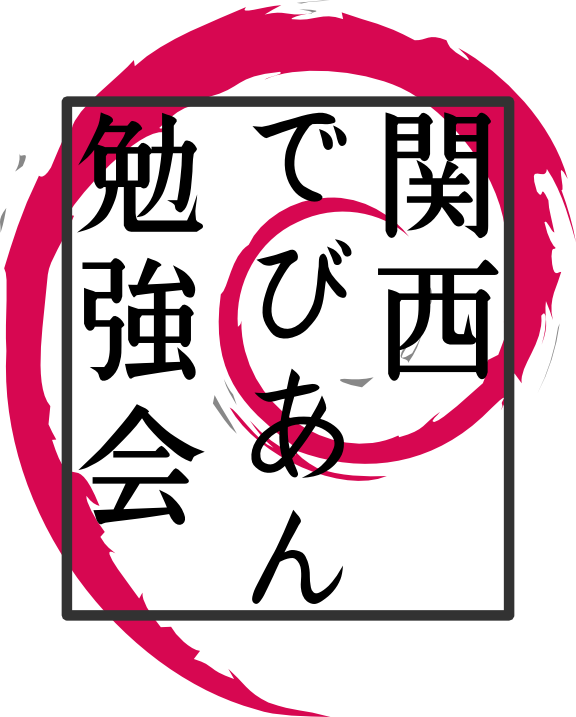
\includegraphics{image200802/kansaidebianlogo.png}
%  \end{center}

% 200908 

\dancersection{Debian Conference 2009参加報告}{岩松 信洋}
\label{sec:debconfreportsummary}
\index{Debconf 2009}

\subsection{Debconfとは}

2009年度の Debconf は 6月23日から6月30日まで、スペインのエクストラマドゥーラで行われました。
日本からは、武藤 健志、前田 耕平、山根 秀樹、岩松 信洋が参加しました。

\subsubsection{Debconfの歴史・経緯}

Debian Conference \url{http://debconf9.debconf.org/} は Debian 
の開発者たちが一同に介するイベントです。通常顔をあわせることのないメンバー
たちが一同に介し友好を深め、技術的な議論を戦わせます。過去の開催履歴を見
てみると\tbref{tab:debconflist}のようになります。

\begin{table}[H]
\caption{歴代のDebconf参加者推移}
\label{tab:debconflist}
 \begin{center}
 {\footnotesize
 \begin{tabular}{|c|c|c|r|}
 \hline
 年 & 名前 & 場所 & 参加人数 \\
 \hline
 2000 & debconf 0 &フランス ボルドー & \\
 2001 & debconf 1 &フランス ボルドー & \\
 2002 & debconf 2 &カナダ トロント & 90名 \\
 2003 & debconf 3 &ノルウェー オスロ & 140名 \\
 2004 & debconf 4 &ブラジル ポルトアレグレ &  150名 \\
 2005 & debconf 5 &フィンランド ヘルシンキ & 200名 \\
 2006 & debconf 6 &メキシコ オアスタペック & 300名 \\
 2007 & debconf 7 &英国スコットランド エジンバラ & 約400名 \\
 2008 & debconf 8 &アルゼンチン マルデルプラタ & 約200名 \\               
 2009 & debconf 9 &スペイン エクストラマドゥーラ & 約250名 \\
 \hline
 \end{tabular}
 }
 \end{center}
\end{table}

\subsubsection{Debconf 2009}

2009年度のDebconfの会場はエクストラマドゥーラ州のカセレス(Caceres)にある
州が管理する施設を活用しました。
スペインのネットワーク会社であるtelefonicaの協力によって、専用のネットワー
ク回線を会場中にはりめぐらせ、無線LANメインのネットワークを構築しました。
(アクセスポイントにはOpenWrtを使っていたようです。)
宿泊は会場にある宿泊施設と、会場から徒歩15分程度に位置する Francisco de Sande に分散していました。

\subsection{スペイン/カセレス}

\subsubsection{行き方}
  行き方としては空路を使った場合、日本からスペイン/マドリッド、マドリッドからカセレスという順になります。
  日本からマドリッド(バラハス国際空港)までは直行便がありません。どこかでトランジットが必要になります。
  各メンバはタイ国際空港経由で入国しました。
  距離は約10000km。飛行時間は約21時間かかります(日本からタイまで約5時間、タイからマドリッドまで約16時間)。
  バラハス国際空港からマドリッドの市街に移動し、さらに列車で4時間ほど移動する必要があります。
  列車のチケットは予約する必要があり、座る場所も決まっています。マドリッドにある
  ターミナル駅、アートチャ駅で購入することも可能ですが、日本チームはインターネットでチケットを予約し、
  印刷して持っていきました。

\subsubsection{会場}

\begin{wrapfigure}{r}{11cm}
  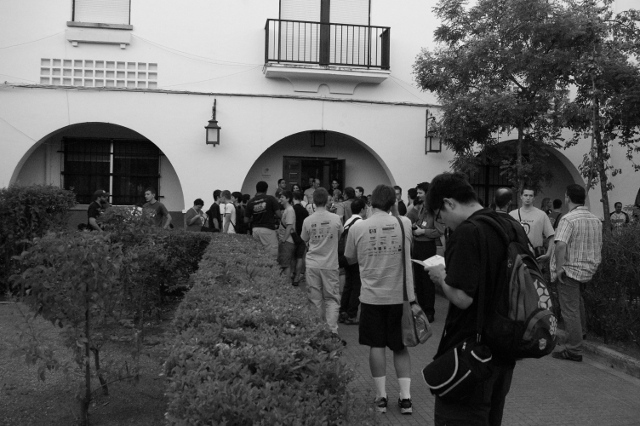
\includegraphics[width=5cm]{image200908/debconf9_venue_mono.jpg}
  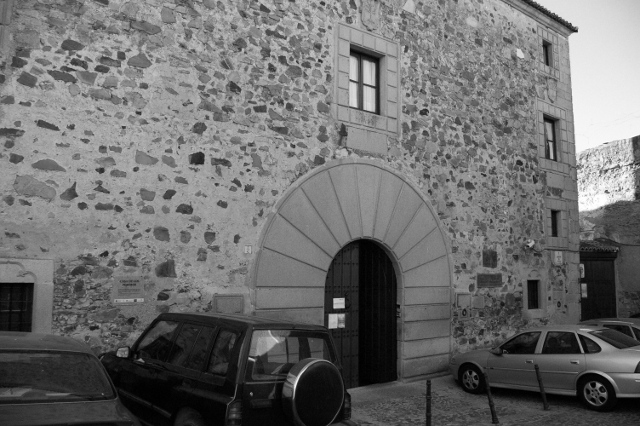
\includegraphics[width=5cm]{image200908/debconf9-fds_mono.jpg}
\end{wrapfigure}
  会場は、エクストラマドゥーラの施設を借り切って開催されました。
  先に書いたとおり、宿泊施設が併設されており、4割の参加者は併設した宿泊施設から
  参加していました。もう片方の宿泊施設である Francisco de Sande は世界遺産である遺跡の
  中にあり、ゲームに出てきそうな宿でした。
  併設された宿泊施設には発表者やメイン開発者が泊まっており、ここでも格差社会が見え隠れしています。
  debconfの前にやっているdebcampと呼ばれるものがあり、こちらは開発が主体になっています。
  開発メインで行いたい人はdebcampから参加するとよいでしょう。
  \\

\begin{itemize}
  \item Upper Talk Room: 	メイン用。250人ほど入ることができます。\\
	\begin{minipage}{0.4\hsize}
	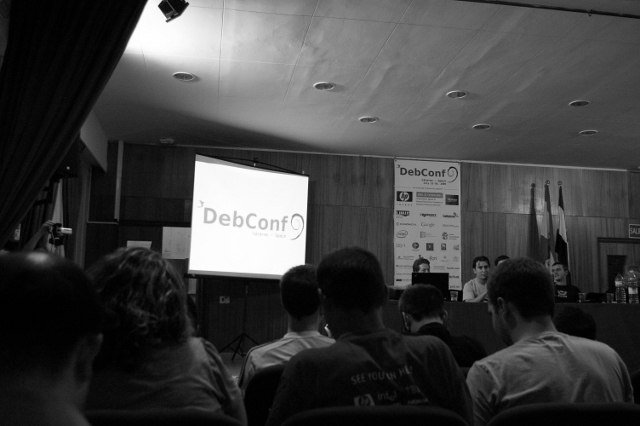
\includegraphics[width=0.8\hsize]{image200908/debconf9_main_mono.jpg}
	\end{minipage}
  \item Lower Talk Room: サブ会場。50人ほど入ることができます。

  \item BoF Room\\
	BOF 用。30人ほど入ることができます。
        プレゼンテーション設備がないため、皆パソコンを開いてプレゼンテーション資料を見ていました。
	また、空調設備が貧弱なため、蒸し風呂状態でした。

  \item Hacklab 1/2 および 食堂: Hacklab はハック専用の部屋です。\\
	\begin{minipage}{0.4\hsize}
	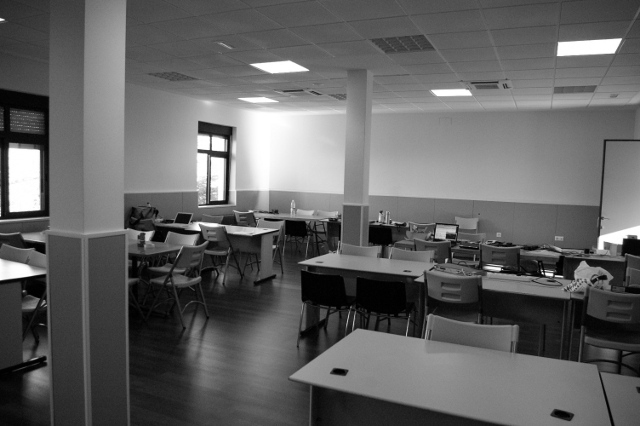
\includegraphics[width=0.8\hsize]{image200908/debconf9_hacklab_mono.jpg}
	\end{minipage}
	\begin{minipage}{0.4\hsize}
	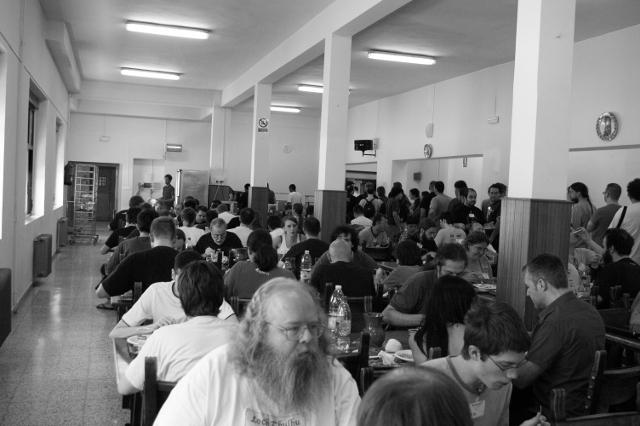
\includegraphics[width=0.8\hsize]{image200908/debconf9_diningroom_mono.jpg}
	\end{minipage}

\end{itemize} 

\subsection{スケジュール}

23日のDebian Day で Debian Conference は開幕し、30日まで毎日いろいろな予
定が組まれていました。
27日だけはカンファレンス参加者で day-trip を実施しました。

\subsection{主となった討論}

\subsubsection{i18n関係}
今回も4回のi18nセッションが設けられ、リリースノート翻訳、DDTP、Wikiをつ
かった 翻訳などの検討が行われたようです。
DDTP翻訳パーティを検討されているようなので、日本からも参加できるようにし
たいところです。

\subsubsection{組み込み関係}
組み込み関係のセッションは全部で9つあり、組み込みからマルチアーキテクチャ
サポートなどが議論されました。

\subsubsection{Multiarch round table}
\subsubsection{Openmoko Buzz Fix Party}
カンファレス参加者に格安で提供されたOpenMokoのバグフィックスパーティ。
OpenMokoはフリーな携帯電話なのですが、日本では使えないので、購入はしませ
んでした。買った人に見せてもらったのですが、なかなかよさげです。Android
も動きますし。ただ、うまく携帯としてつかえないことがあるようで...(以下
略。
\subsubsection{Mer: Maemo Reconstructed}
Maemo のコミュニティ向け環境 Mer についての説明。
タブレットPC向けのようですが、N8XXやOpenMokoでも動作するようです。

\subsubsection{Scratchbox2 for crosscompiling debian}
Riku がメンテナンスしている Scratchbox2を組み込み環境でどのように利用す
るのか、という話。scratchboxでツールを作成し、scratchbox qemu のフロント
エンドとして利用したパッケージ作成ができるようになったので皆で使いましょ
う。

\subsubsection{uclibc and busybox}
uclibc と busybox Debianでどのようにサポートしたらいいのかという話。
emdebianで busyboxベースのdebian環境をサポートするために頑張っているよう
です。これらについての意見交換をしました。
sh4 もサポートに入る予定です。

\subsubsection{emdebian BoF}
毎回恒例になっている emdebianの進捗報告。
emdebianでは、Emdebian Grip と Emdebian Crush の2つのプロジェクトが
進行中。前者は busybox/uclibc ベースの debianを、後者は 現在のDebianをク
ロスコンパイルサポートするプロジェクト。emdebian-toolsができて、ある程度
ましになったけど、まだ不具合が多いので開発者募集中。apt-crossは依存関係
の実行がまだまだなので、今後力をいれて開発していくとのこと。
私からはsh4のサポートもするから協力しろ、と言っておきました。

\subsubsection{QEMU for Debian Developers}
aurel32 によるフリーのCPUエミュレータであるqemuの進捗状況と使い方につい
て。Debianでサポートしてるアーキテクチャのほとんどはqemuでサポートしてい
るのでマシンが手元になくてもデバッグできるよ、という話。
イメージも彼のWebサイトにあるので、mips や ppc などを試したい人はどうぞ。

\subsubsection{Crossbuilding on Debian for a derived distro}
既存のLinux組み込みシステムからDebianのシステムに移行した時の話とツール
の使い方、クロスコンパイルの方法についての話。
発表者のWookyは去年から会社が変わったのですが、システムをDebianに移行し
たので、そのときに行った方法を話していました。
CMakeでのクロスコンパイルが面倒だったようです。

\subsubsection{xcontrol}
Simon が毎年やっているxcontrolの話。debian/controlファイルを拡張してクロ
スコンパイルパッケージや、バックポートのサポートを容易にしましょうという
セッション。前回から進展があったのかは不明です。

\subsection{ツール関係}

\subsubsection{News on Debian Autobuilding}
buildd の現状と問題点の報告。
dep-wait、failedの遅延への対応や、パッケージプライオリティに対応したビルドについ
て議論されました。

\subsubsection{Trust is good, control is better}

パッケージのインストール、アンインストールのチェックができるpiupartsの進
捗報告。HPのマシン2台を使って、すべてのパッケージのチェックを定期的に行っ
ています。これにより、次期リリースではパッケージのインストール、アンイン
ストールが問題なくできるようになるでしょう。

\subsubsection{Using FOSSology for license analysis in Debian} 

tbm によるコードライセンス解析ソフトの話。deb, rpm,tarボールなどをリポジトリに食
わせライセンスの構文解析を行った結果をDBにまとめているとのこと。
ライセンスとCopurightがどのように変化していったのかまで調査できるようで
す。デモをしていましたが、ちょっと動きは遅いかな。
今後に期待です。\url{http://fossology.org/}

\subsubsection{not your grandpa's debhelper}

Joeyによるdebhelperの解説。debhelperはdh\_\*のプログラムを提供しますが、
これらをまとめたコマンド dh を作りましたという話。
dh を使うとdebian/rules を以下のようにまとめることができます。
\begin{commandline}
#!/usr/bin/make -f
%:
  dh: $@
\end{commandline}
各ターゲットもオーバーライドすることができて、override\_dh\_xxxx を作成し
ておくと呼ばれるようになります。dh 勉強会とかやりたいですね。

\subsubsection{UDD: Ultimate Debian Database}
% From http://kmuto.jp/d/index.cgi/travel/20090726-spain.htm
Debian/Ubuntuのパッケージ情報やpopcon情報、debtags、LDAP、アップロード履
歴、DDTP、testingミグレーション、バグ、NEWキュー、lintian、スクリーンショッ
トURL等々といった情報を全部PostgreSQLデータベースに突っ込んでデータマイ
ニングしてみました、という話でした。
これらのデータベースはmerkelとaliothで提供されています。
インターフェイスは公開されているので、誰でも試すことができます。


\subsubsection{pam-auth-update: manhandling debconf for fun and profit}
       squeezeから新しく導入された、pam-authの設定ツールです。今までは、
       /etc/pam.d/以下を手動で設定していましたが、/usr/share/pam-configs 以下の
       テンプレートを使い、postinst, prerm の中で、pam-auth-update コマンドを実
       行することで簡単に pam-auth の設定をできるようになります。3rd party 製の
       ツールも、これに則れば簡単に導入出来るようになるので、ユーザにとってもと
       てもメリットが大きいでしょう。Sid の環境では、次のファイルが既にこの制御
       下にあるようです。
 \begin{itemize}
  \item /etc/pam.d/common-account
  \item /etc/pam.d/common-auth
  \item /etc/pam.d/common-password
  \item /etc/pam.d/common-session
 \end{itemize}


\subsubsection{Changing the default system shell}
       デフォルトシェル /bin/sh をなぜ変えるのか?ポリシーもあるようです
       が、切り替える一番の動機としては、遅いからだということを言ってい
       ました。bash で記述されたものは約800あるうち、fix 済みのものは
       160 だそうです。bash を検出するには、devscripts, lintian, archive
       rebuilds, piuparts, ユーザの報告があるそうです。最終的には自分で
       判断して bash にするのをやめ、dash を選択するようにしてほしいと言っ
       ていました。

\subsubsection{DDE, Debian Data Export}
      Debian に関する情報を HTTP プロトコルで取得することができる
      RESTful アプリケーションのようです。
      \url{http://dde.debian.net/dde} や
      \url{http://debtags.debian.net/dde} から、データを取得することがで
      きます。

\subsubsection{Libvirt: Hypervisor independent virtual machine management}
       libvirt という仮想マシンを扱うための API の話です。Debian 固有の話
       は特になく、libvirt の紹介をしていました。Debian でもちゃんと使え
       るようなので、ぜひ使ってみましょう。

\subsubsection{RFH maintaining big packages}
       iceweasel のパッケージメンテナの Mike さんの BOF。iceweasel, OOo
       では、どうやってユーザや開発者をより多く巻き込んでいくか、活動を
       宣伝していくか、という点で議論が交わされました。

\subsection{リリース関係の話}
\subsubsection{Keynote from the Release Team}
Release team によるキーノート。Debianからのニュース
\url{http://www.debian.org/News/2009/20090729}でも流れているように
この場で、次期安定版であるSqueeze のフリーズとタイムベースリリースの話が
出ました。うまく行くか不安ではありましたが、その場ではいけるんじゃね?とい
う空気になっていました。(案の定、MLではフレームになっていますが。)

\subsubsection{GPGサイン}
Debconf9開催前にDSAの脆弱性が発覚し、これにより新しいGPG鍵を作成する
必要がでてきました。新しく作成した鍵を使って開発者同士で鍵サインをする必要が
出てきたため、今回のDebconfではGPGサインが活発に行われました。
今回のポイントはこれまでの事務的な手続きを反省して、Debconf開始に際してセッションを開き、
チェックサムの検証を行って、あとは好きなときにちゃんと相互におしゃべりをしながらサイン交換しましょうということがとても重要だったと思います。
名札にGPG鍵リスト上で割り当てられた番号が書かれていて、やりとりを促進するようにもなっていました。おかげで我々は29日夜のサインパーティに出られないながらも、
hacklabや食事どき、デイトリップの最中などいろいろな場面で多数サイン交換ができました。

武藤さん、岩松は40名ぐらいの参加者と交換することができました。

\subsection{Daytrip}

\begin{wrapfigure}{r}{5cm}
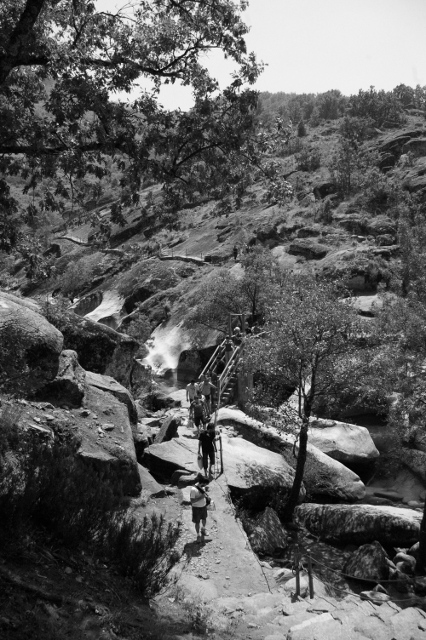
\includegraphics[width=5cm]{image200908/debconf9_daytrip_mono.jpg}
\end{wrapfigure}

Debconf では一日、参加者で旅行をするというイベントがあります。今回の
Debconfでは 会場からバスで2時間ほど移動したところにあるエクストラマドゥーラ州が
運営しているキャンプ場に移動し、そこから1時間ほどハイキングをしました。
ハイキングの先には、自然でできたプール(Natural Pool)があり、そこで皆で泳いだり飛び込んだり、
滝に打たれていました。一部溺れかけてた人もいたようですが、皆無事だったようです。
4時間ほどそこで遊んだ後、別の場所に移動し、みんなでビールを飲みました。
そこにも川をせき止めたプールがあるのですが、皆のグランパであるJoeyが足を
ざっくり切ってしまうイベントが発生し、救急車が呼ばれるハプニングがありました。

\subsection{Debconf11}
Debconf11 はボスニアとドイツが立候補しました。
ドイツはまだ場所が決まっていないようですが、今年中に場所を確定させるよう
です。ボスニアはトランジットが面倒ですが、開催地は空港から数キロのところ
にあり、そんなに困らないように感じました。
ドイツはDebian開発者が一番多い国で、Debconfチーム(orga)のメンバも多いた
め、ドイツ濃厚な気がします。

\subsection{今回のDebconf参加によるハックの成果}
\subsubsection{武藤さん}

ツアーコンダクターとして、マドリード観光や現地での皆さんの安全・食事探しに取り組みました。

\begin{itemize}
\item ドラゴンクエストIX\\
  出発時には最初の村を出るところでしたが、移動時間中だけで遊んでいたにもかかわらず、成田に戻る飛行機ではラスボスと戦っていました。全滅してしまったのでもう少し経験を重ねたいと思います。
\item フリーソフトウェアマップの翻訳\\
  スペインでフリーソフトウェアの活動を進めているGNUプロジェクトメンバーのRene Merouに頼まれて、彼らの作っているフリーソフトウェアマップを日本語に翻訳しました。政府機関にフリーソフトウェア採用を働きかけるなど、活発な活動をしているそうです。
% image200908にmap-ja.svg、map-ja.pngとしてコミット。どうリンクするとよい?

% \begin{wrapfigure}{r}{5cm}
% 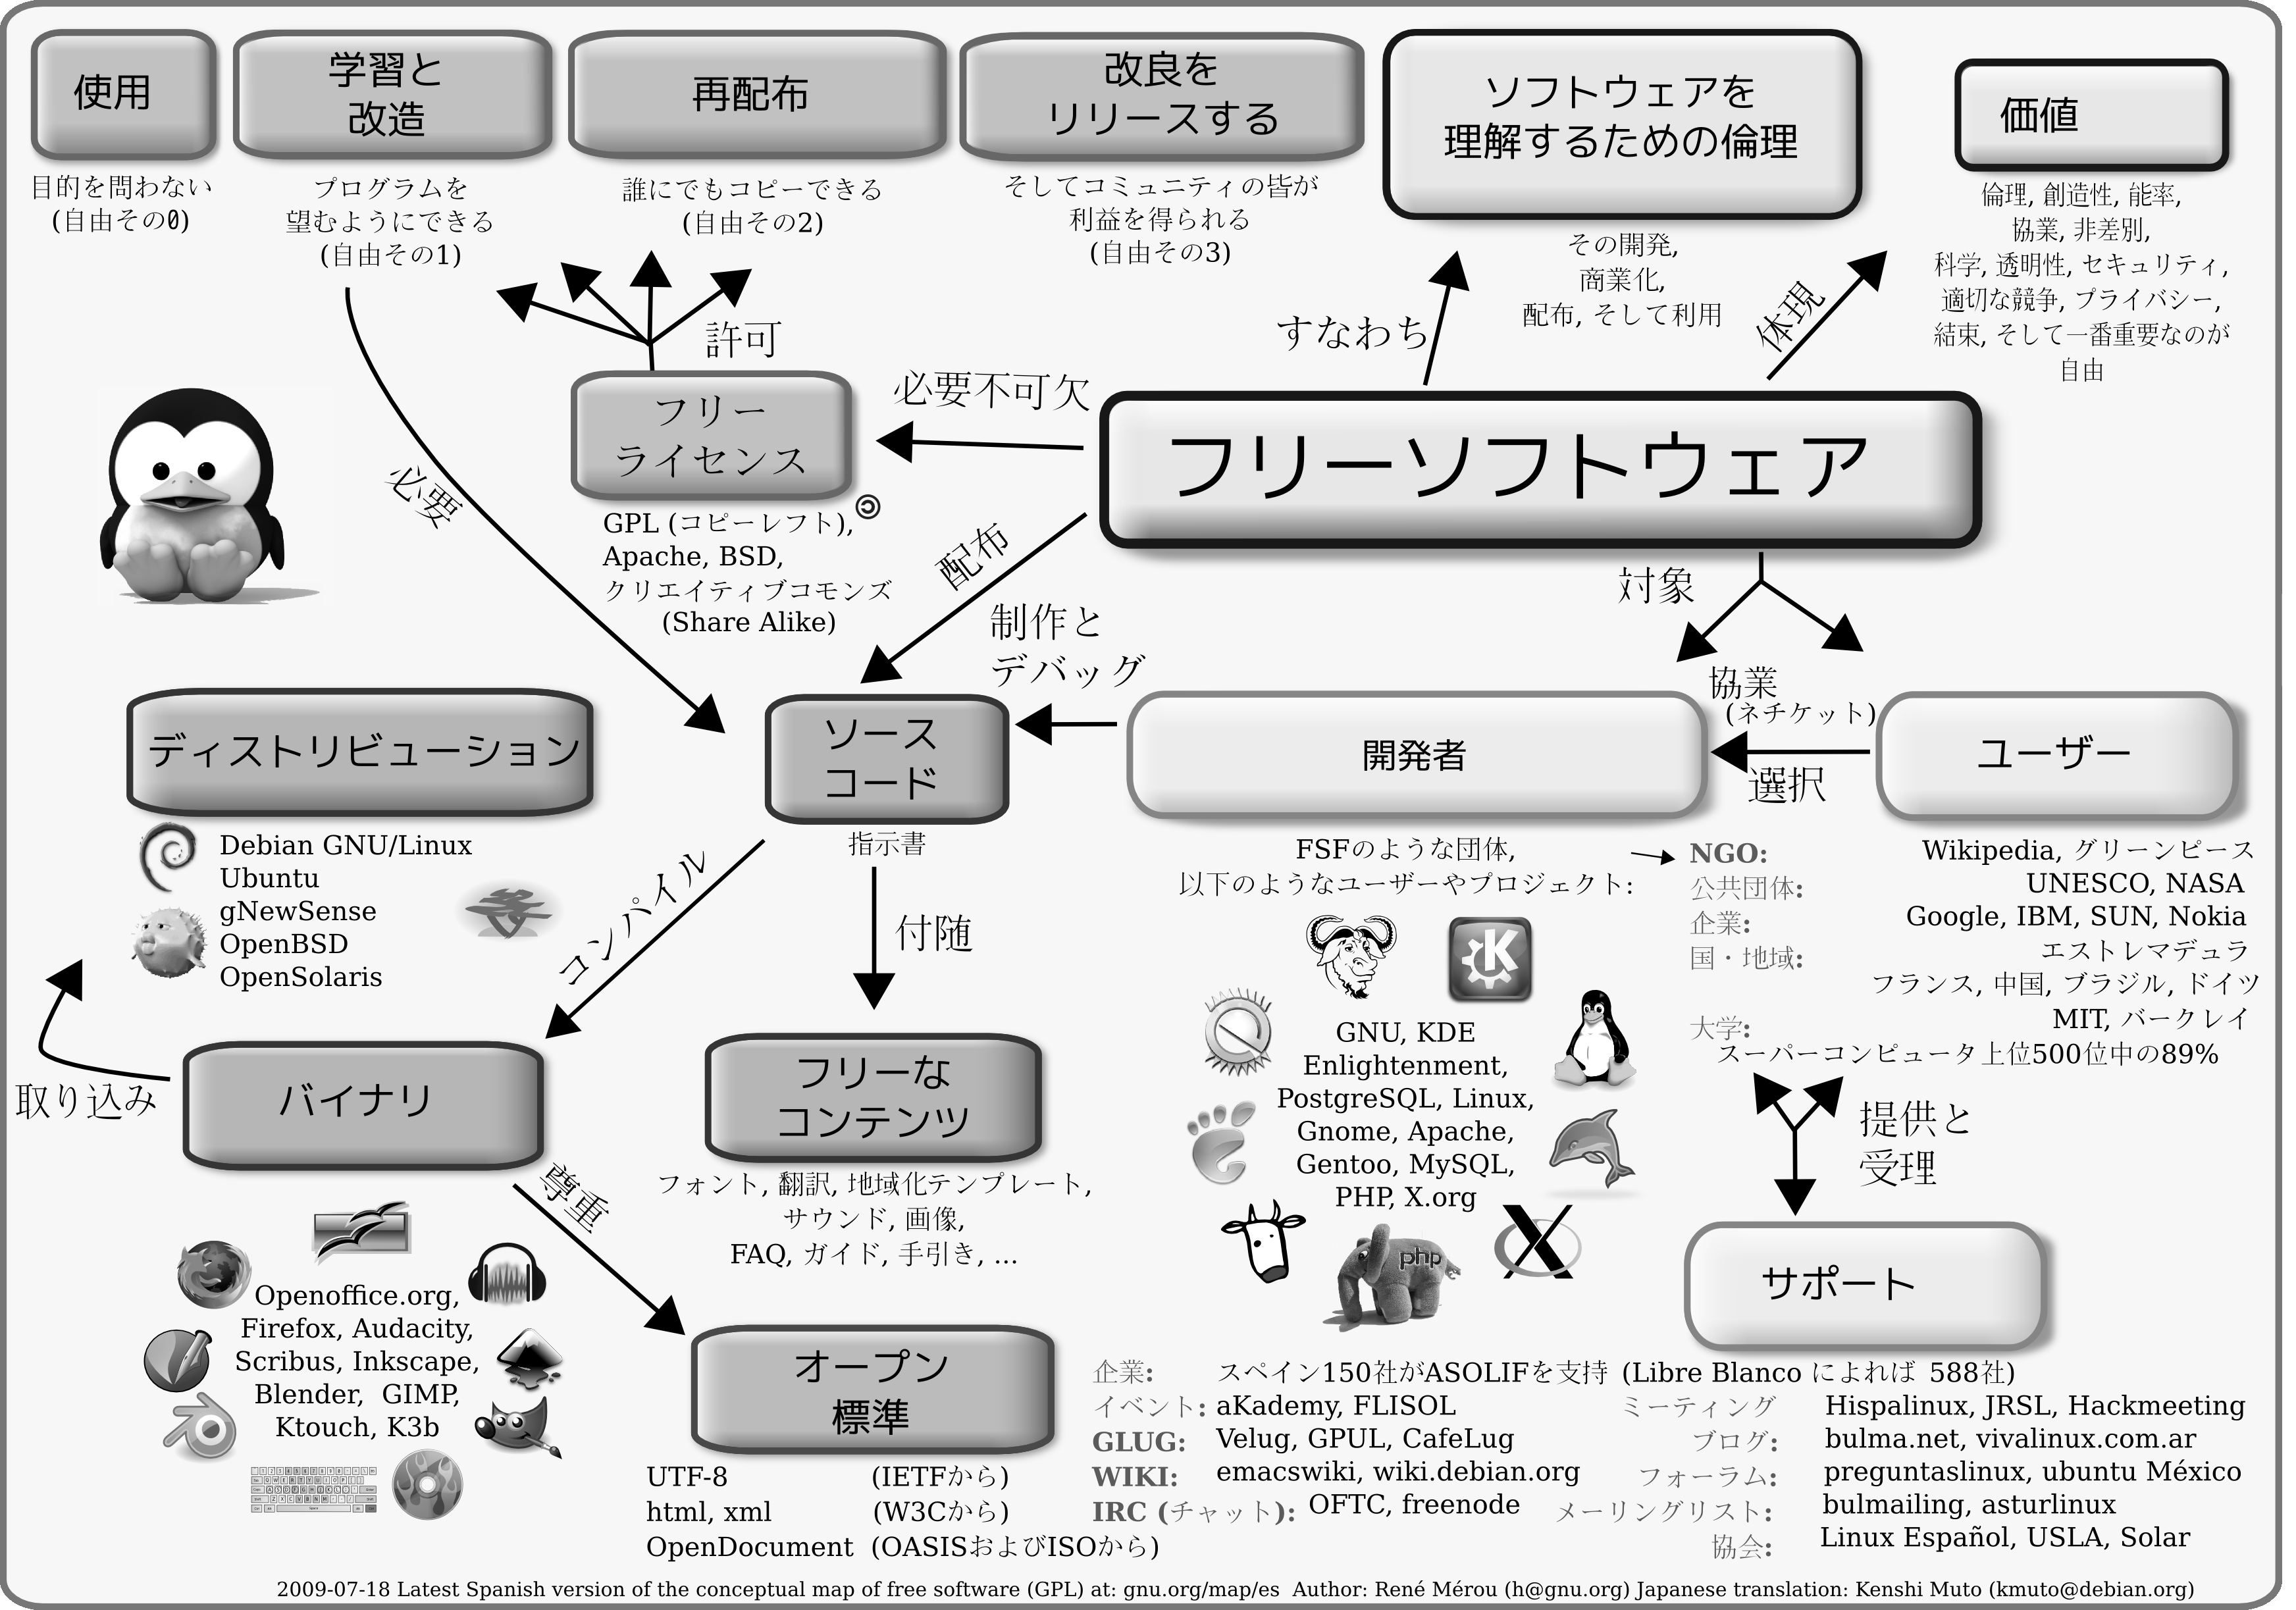
\includegraphics[width=5cm]{image200908/map-ja_mono.png}
% \end{wrapfigure}

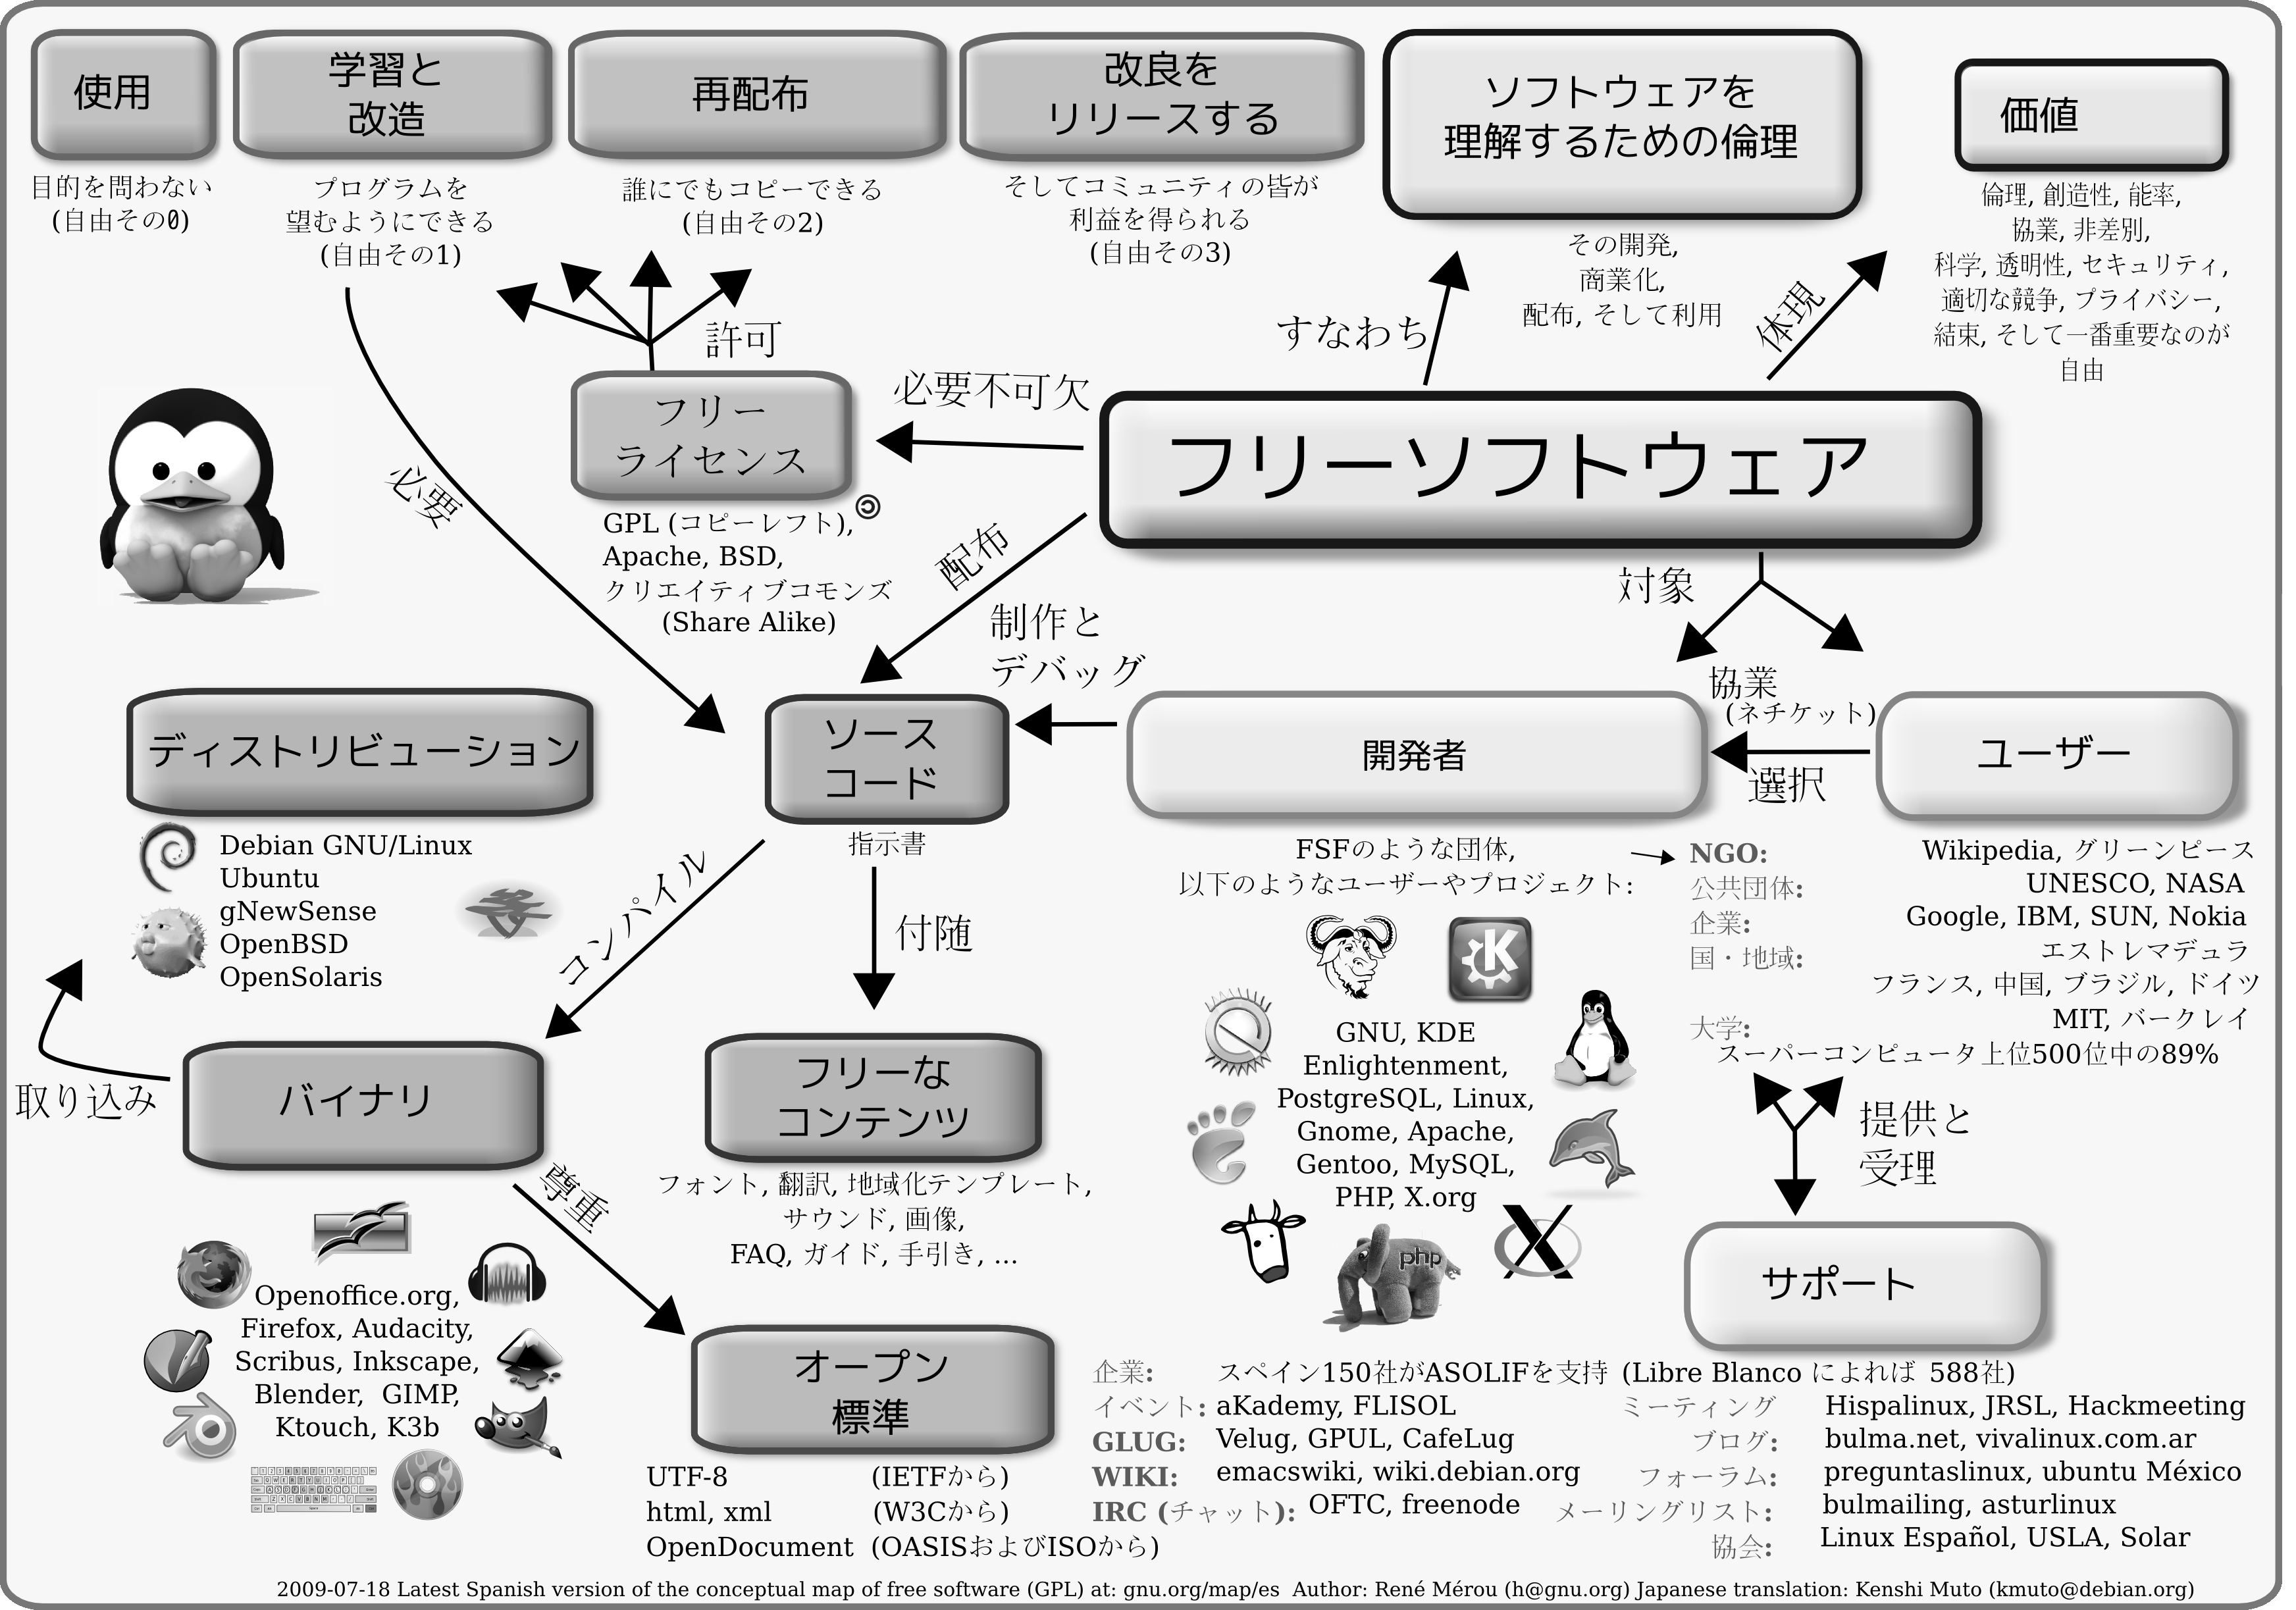
\includegraphics[width=15cm]{image200908/map-ja_mono.png}

%\begin{minipage}{0.4\hsize}
%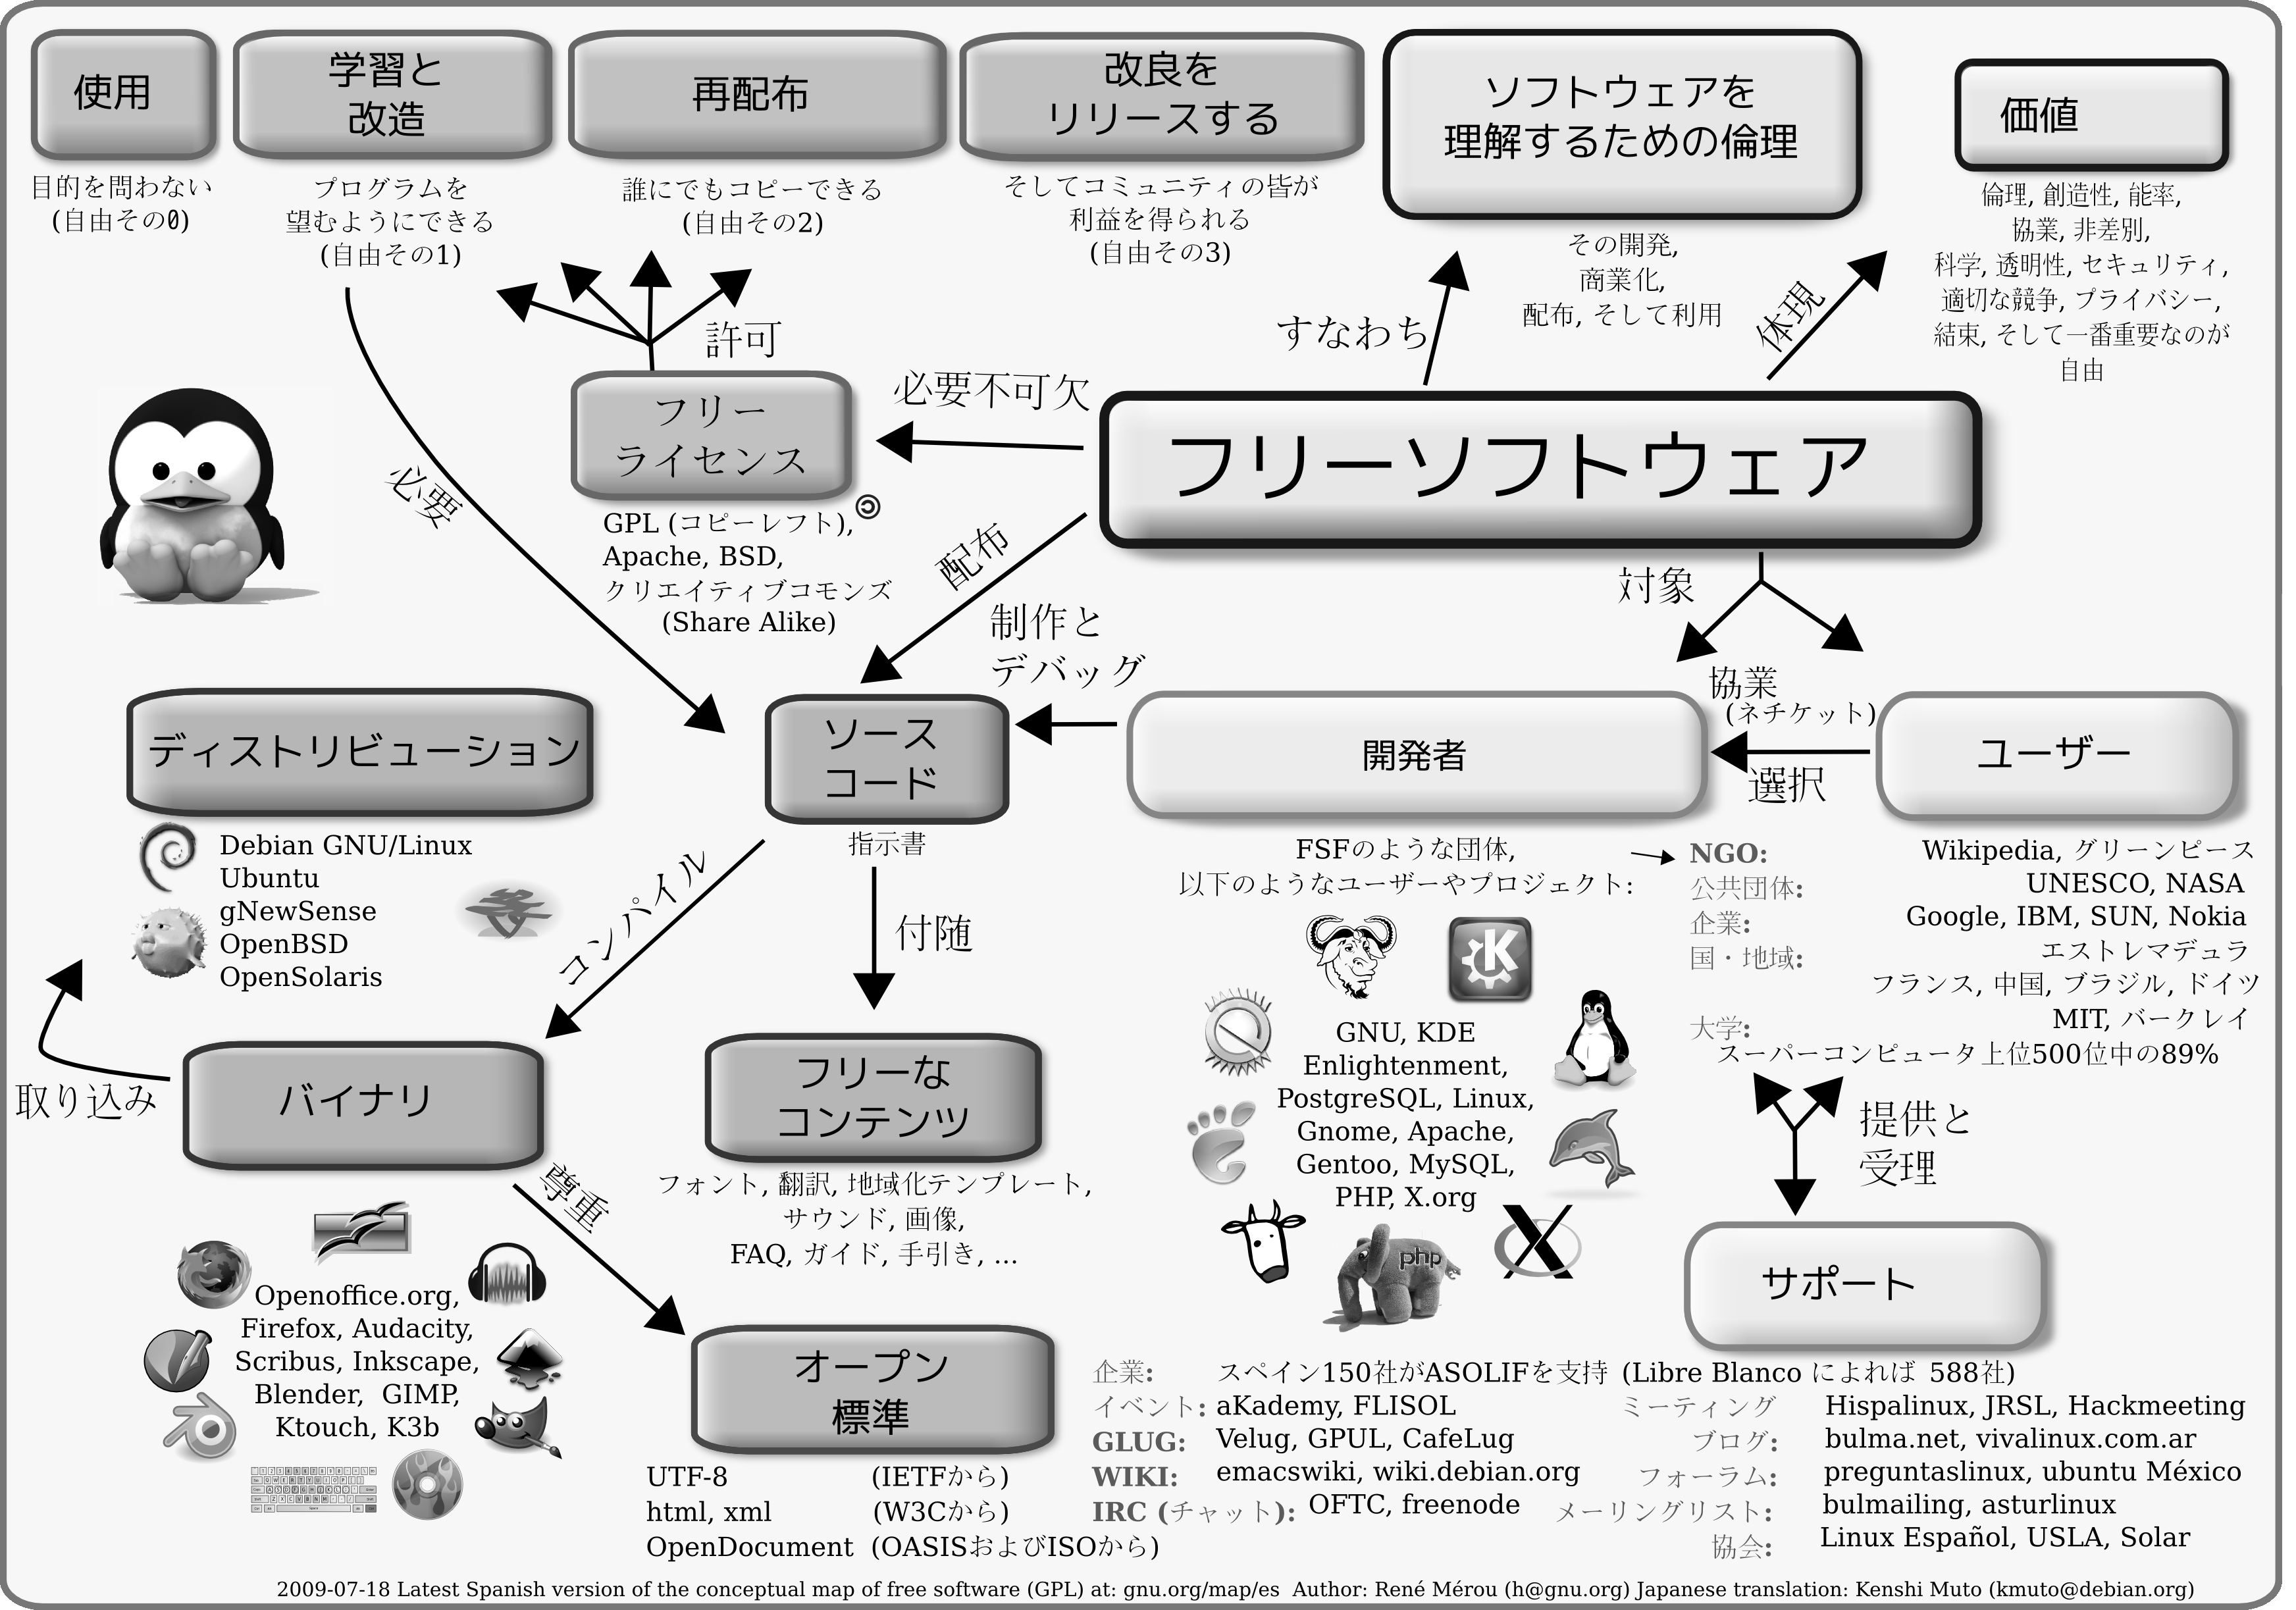
\includegraphics[width=2.0\hsize]{image200908/map-ja_mono.png}
%\end{minipage}

\item ハードウェア互換性リストとハードウェアサポートページの友好関係構築\\
  Debianのハードウェアサポートの情報を収集してWiki(http://wiki.debian.org/HardwareDatabase, http://wiki.debian.org/DeviceDatabase/PCI など)にまとめているFranklin Piatに会って、私のDebian HCL(http://kmuto.jp/debian/hcl/)とどのような協業ができるかを話し合いました。まずは彼のUSBデータベースの成果を生かして、lsusbコマンドを貼り付けることでUSBのサポート情報を表示するようにHCLを拡張できるかを検討することになりました。
\item 国際化チームミーティング\\
  恒例の国際化チームミーティングは期間中4回開催され、WikiやDDTPについて議論がなされました。SqueezeではリリースノートをWikiベースで制作・編集するというトライアルが実施されます。Wikiのように変動の激しいものを翻訳するための手法として、poフォーマットに変換してパラグラフ単位で作業できるような手法も実施予定です。Debianのパッケージ説明翻訳機構のDDTPについても、多数の改善提案が出されました。パラグラフ単位でのマッチングやfuzzyマーキング、一般翻訳者を統轄するコーディネータという役割および特権を用意して一括置換や管轄する翻訳メンバーへの一斉連絡といった機能が追加される見込みです。日本のDDTP翻訳チームでも、いずれどなたかにコーディネータに立候補いただくことになると思われます。
\item 講演レポート\\
  各講演内容については
  \url{http://kmuto.jp/d/index.cgi/travel/20090722-spain.htm}, \\
  \url{http://kmuto.jp/d/index.cgi/travel/20090724-spain.htm}, \\
  \url{http://kmuto.jp/d/index.cgi/travel/20090726-spain.htm}, \\
  \url{http://kmuto.jp/d/index.cgi/travel/20090728-spain.htm}  \\
  に短いながら報告しています。詳細についてはDebianの関連メーリングリストやDebconfサイトで掲載予定のビデオなどを参照してください。
\end{itemize}

3年ぶりの参加でしたが、新旧の友人たちと語らい、GPGサイン交換し、Debconf初参加者にDebconfを体感してもらい、国際化チームミーティングでup-to-dateな情報を得る、と当初の目的はいずれも達成できました。充実したカンファレンスだったと思います。

私自身は今後徐々にDebianに関する活動のペースを落としていくつもりなので(すでにだいぶ落ちてしまってはいますが)、特にDDTP関係者のDebconfおよび国際化チームミーティングへの参加を望みます。

\subsubsection{山根さん}

 兎に角、「参加することに意義がある」と言うことで参加してみました。初海外だったのでドキドキものです。色々と皆さんに助けていただきました。

\begin{itemize}
 
 \item po-debconf 訳\\
       多少は fuzzy, unstranslated を潰しました。
 \item フォントパッケージのライセンス確認\\
       日本語フォントについて、何故かスペインについてからupstreamに確認を取り始める私。
       「OFLだよ」「完全にフリーです、著作権も行使しません」との返答を得ました。
       パッケージにするのはdescriptionとdefoma-hintsファイルの作成が待ってますが…
 \item 参加レポート\\
       これとは別にまた少しだけ書いておこうと思います。
 \item GPG keysign\\
       15、6人ほどと鍵交換したはず。caff便利なんですね。そのうち使い方とかまとめたいかも。
 \item java policy 訳 review\\
       帰りの飛行機で半分ほどをレビューしました。何故。
\end{itemize}

 逆に課題としてもらってきたのは「英語英語英語〜」ですね。かなり精進が必要な模様です。

\subsubsection{前田さん}

数ヶ月溜まっていたタスク、問題を ToDo として取り組みました。

\index{MacBook}
\begin{itemize}
 \item MacBook 5,2 の使えないデバイスを使えるようにする\\
       所有している MacBook は 2008 later モデル(通称 MacBook 5,2)ですが、
       DebConf に行く前に以下のような問題を抱えていました。

       \begin{itemize}
	\item 無線 LAN を使えない \\
	      Broadcom bcm4322 が搭載されており、b43 で将来的にはサポー
	      トされるらしいのですが、現状では Broadcom が提供している
	      STA ドライバを使用するしかありません。ただし、普段、
	      vanilla kernel の最新 stable を使用していると、このデバイ
	      スドライバをビルドできない、という問題があります。スペイン
	      から Twitter でつぶやいていたら、Gentoo の松鵜さんに、
	      Gentoo のパッチを使ってみては、と教えていただき、x86用のパッ
	      チを参考に、amd64(x86\_64) 用にコードを書き直したところ、
	      正常に無線 LAN を使えるようになりました。

	      実は Debian に既に Broadcom-sta ドライバ用のパッケー
	      ジがあり、これを使うと上記の問題は既に解決されている、とい
	      うオチもついてました。\footnote{broadcom-sta-common,
	      broadcom-sta-source パッケージ。i386 用にはバイナリパッケー
	      ジもあるようです。}
	      \index{broadcom-sta}
	\item 音が出ない \\
	      サウンドデバイスは認識しているものの、音が出ない、という現
	      象にハマっており、/etc/modprobe.d/alsa-base.conf の設定を
	      しなおすことでシステムブート時に音が出るようになりました。

	      が、これが非常にけたたましいビープ音で、イヤホンジャックに
	      イヤホンを挿してもなりやまず、Hacklab1 内でかなり顰蹙(ひん
	      しゅく)を買ってしまいました…。orz

	      帰国してから再設定したのですが、再び音が出なくなり、四苦八
	      苦中です。
	\item iSight が対応していない \\
	      isight-firmware-tools が、MacBook 購入時(2009年5月末)では
	      対応していなかったのですが、久しぶりに実行してみたら何もす
	      ることなくあっさりファームウェアを抽出でき、使えるようにな
	      りました。
	\item ACPI を有効にすると起動できない \\
	      この問題は未だ解決しておらず、ACPI を無効にするためバッテ
	      リー駆動の場合、残量が分からないとか、正常に電源を切れない
	      ため reboot ができず必ず shutdown しないといけないとか、ハ
	      イバネーションを行うと、復帰時に ACPI を有効にしたときと同
	      様に画面がブラックアウトして固まってしまう、という問題があ
	      ります。
	      
	      DebConf で MacBook を使っている人に聞いてみようかと思って
	      いたのですが、同じ世代の MacBook を使っている人が少なく、
	      持っていても Mac OS X を使っているので、断念しました。

	      ACPI の ML で聞いてみる予定です。
       \end{itemize}

 \item Java Policy の翻訳 \\
       4月の Debian 勉強会のネタとして、Java Policy を読んでみましたが、
       中途半端なところで翻訳を中断していました。再開するにあたり、PO 形
       式で整形し直し、未翻訳の部分の翻訳を完了し、debian-doc に投稿しま
       した。

       レビューコメントをやまねさんに頂いたのですが、帰国してから飼いは
       じめたネコに夢中で再び停滞しているので、今回の勉強会後に確認し、
       修正後、Java Policy のMLへの連絡及び、java-common パッケージのBTS
       を行う予定です。

 \item GanttProject のパッケージ化 \\
       ソースコードの入手方法が分からず、放置していたのですが、
       Subversion のリポジトリがあることに気づいたので、ドキュメントに沿っ
       てビルドしてみたところ、OpenJDK では正常に動くことを確認しました。

       他の Java 開発環境でのビルド、動作確認後、deb パッケージ化を行う
       予定です。

 \item Termtter のパッケージ化事前調査 \\
       jugyo さんが中心になって開発されている Twitter のターミナルクライ
       アントがあります。iceweasel の extention である twitterfox の使い
       勝手がいまいちなのと、ちょうど DebConf9 中に動作がおかしくなり、
       有効にしていると iceweasel ごと busy になってしまうので、切り替え
       ることにしました。使い勝手がよければ、deb パッケージにしてしまお
       うと考え、KVM環境で検証してみたところ、rubygems で必要なライブラ
       リを導入し、既に deb パッケージで導入済みのライブラリを無視してし
       まいます。

       今後の予定としては、その当たりの解決と、gems で導入されている deb
       パッケージになっていないライブラリ自体のパッケージ化の検討を行う
       つもりです。

 \item おまけ1。最近中古で買ったスーパーマリオブラザース DS をクリアしま
       した。クッパに息子がいるとは。またクッパはゾンビなってしまったのですね。

 \item おまけ2。最近、帰国後から飼い始めたネコですが、帰国後に引き取りに
       行くことが決まっていたので、事前にネコの健康本と、ネコの気持ちが
       分かる本を買っていきました。、帰宅後、熟読して帰ったらヨメにネコ
       博士と呼ばれるようになりました。
\end{itemize}

セッションにはいくつか参加しましたが、知らない内容を勉強するために出てみ
ても、英語の聞き取りがほとんど出来ないので、言っていることが分からないと
いう問題にぶち当たりました。そういう場合は、資料が頼りなのですが、事前に
配布されていないセッションも多く、おまけにスライドの文字が小さくて前の方
の席で眼鏡をかけても見えないようなセッションでは、非常に大変でした。

\subsubsection{岩松}
岩松は主に sh4 アーキテクチャ向けの開発を行いました。
\begin{itemize}
\item buildd hack\\
Debian / SH4 の buildd が動きはじめました。これにより、SH4向けバイナリが debian-ports.org
が取得できるようになります。
パッケージ作成の進捗は\url{http://www.debian-ports.org}から参照することができます。
\\
また、armel buildd メンテナである Riku と組み込み向けCPUで発生する問題を
どのようにフックしていくのか、意見交換を行いました。
\item debian kernel\\
tbm \footnote{元DPL, armのカーネルメンテナ} を捕まえて、debian kenrel configファイルのハックをしました。
sh4 向けカーネルサポートを一通りできました。

\item sh4 向けクロスコンパイラのサポートの打ち合わせ\\
gcc のクロスコンパイラサポートをしている zumbi と会話し、sh4 と uclibcのクロスコンパイラ
サポートの話をしました。gcc-4.4 ではうまく動作しないので修正したり、クロスコンパイルに
必要なパッケージを提供したりしていました。

\item defoma\\
defoma を ITA したままほったらかしにしていたので、CPAN adminをつついて、
バグのある CPANの乗っ取りを再開しました。CPANはやりとりが面倒くさいので新しい
ソフトウェアを作成したほうが早そうです。

\item Linux kernel/ U-boot \\ 
こっちに来ている間にもパッチが飛び交っているのでメールのチェックとパッチ
の査読をしていました。

\item speedstep-centrino
自分の使ってるMacBookはCoreDuoなので、speedstep-centrinoが使えるはずなの
ですが、モジュールのロードに失敗します。CPUマニュアルを斜め読みして対応
してみました。

\end{itemize}
\subsection{次回のDebconf}
次回のDebconf10は 米国のニューヨークで開催される予定です。
一部の日本人が日本での開催を再度目論んでいるようです。
スポンサーとか会場情報募集中。

% ===============================================================
\dancersection{Debian GNU/kFreeBSD をインストールしてみよう}{山本 浩之}
\index{kfreebsd}
\index{debian}
% ===============================================================

今年 4 月 5 日に正式に Debian archive に入った Debian GNU/kFreeBSD ですが、
現時点で最新インストーラである debian-20090117-kfreebsd-i386-install.iso 
(2009/1/17製) を使ってインストールしてみました。

英文ドキュメント
\url{http://glibc-bsd.alioth.debian.org/doc/}

\begin{commandline}
wget http://glibc-bsd.alioth.debian.org/install-cd/kfreebsd-i386/current/debian-20090117-kfreebsd-i386-install.iso
\end{commandline}

このイメージにある kernel は、FreeBSD 7.1R のものですが、インストール後、
7.2R の kernel にアップグレード可能です。

今回は VMware の仮想ディスクにインストールを試みました。
インストーラは、現在のところは、FreeBSD 用のものを一部改造したもの
のようです。
インストーラを CD イメージから起動します。とりあえず Express (または Custom)で
インストールしてみましょう。

\begin{minipage}{0.4\hsize}
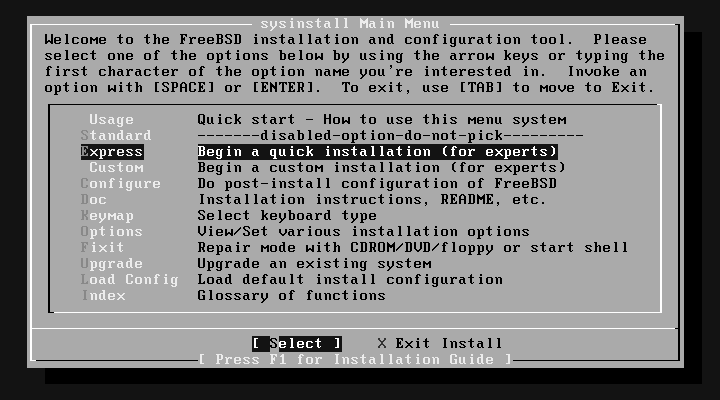
\includegraphics[width=6cm]{image200906/kfreebsd02_mono.png}
\end{minipage}
\begin{minipage}{0.4\hsize}
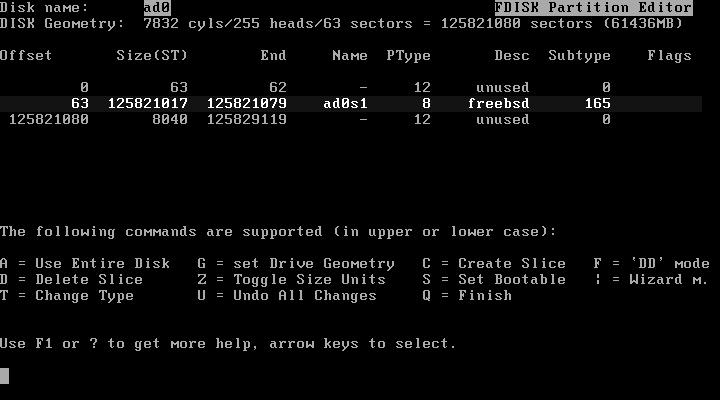
\includegraphics[width=6cm]{image200906/kfreebsd03_mono.png}
\end{minipage}

まず最初にすることは、Linux と同様、インストールするディスクを指定します。
fdisk が起動しますが、ここで注意しなくてはならないのは、Linux とはディスクの
指定の仕方が違うことです。FreeBSD では、hda1 にあたるものは、ad0s1 で、
スライスと呼びます。FreeBSD では伝統的に、使用する領域全部を先にスライス (ad0s1) として確保し、
その中にディスクラベルをつけることによって小分けして(ad0s1a、ad0s1b など)、
それぞれのマウントポイントを作ります。
Linux の場合のパーティションの設定に近いものはディスクラベルかもしれません。
とりあえず "A" で、空き領域全部指定しましょう。

次にブートローダの書き込みですが、デフォルトでは FreeBSD Boot Manager と言う
 FreeBSD 専用のプログラムが使用されます。もし既存の grub が使いたい場合には、
ここでは書き込まず (None を指定)、インストール後に、既存の grub が使っている 
/boot/grub/menu.lst に
\begin{commandline}
title Debian GNU/kFreeBSD
root (hd0,0,a)
kernel /boot/loader
\end{commandline}
とか書けば良いそうです。
仮想ディスクなどに対してのインストールで、マルチブートの必要が無い時は "Standard" を選んでください。
FreeBSD Boot Manager を使ってマルチブートしたい場合にのみ "BootMgr" を選んでください。

\begin{minipage}{0.4\hsize}
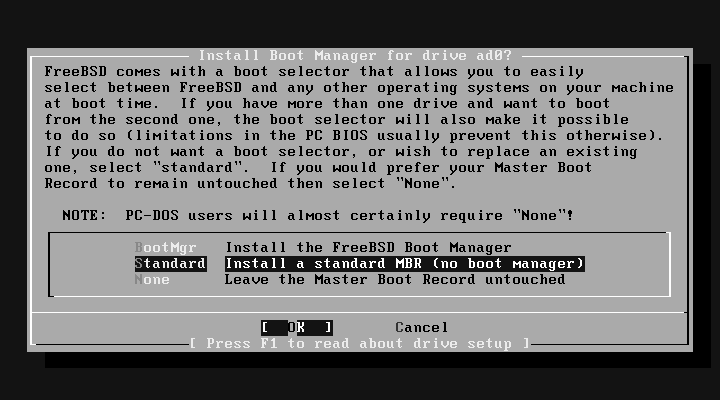
\includegraphics[width=6cm]{image200906/kfreebsd04_mono.png}
\end{minipage}
\begin{minipage}{0.4\hsize}
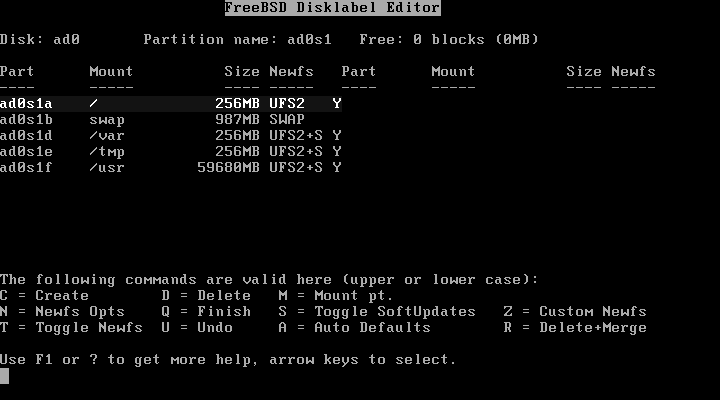
\includegraphics[width=6cm]{image200906/kfreebsd05_mono.png}
\end{minipage}

次に FreeBSD Disklabel Editer が起動し、スライスの中に、
さらにマウントポイントとしていくつもディスクラベルをつけます。
それぞれ ad0s1a ad0s1b ...などとなります。
"/" のため、少なくとも一つはディスクラベルをつける必要があります。
もし、"/usr" とか "swap" とかを分けたいときにはここで選びます。
"A" で、自動的に割り振ることも可能です。

そして Distribution の選択 (Choose Distribution) ですが、
ここでは必ず "A Minimal" を選択してください。
ここで色々な選択肢が出てきますが、これは元の FreeBSD のインストーラだったころの名残りで、
これは Debian のインストーラですから、FreeBSD の Distribution は全く収録されていません。

\begin{minipage}{0.4\hsize}
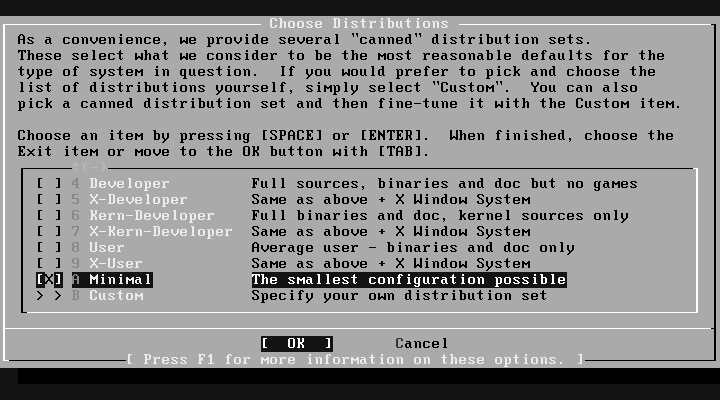
\includegraphics[width=6cm]{image200906/kfreebsd06_mono.png}
\end{minipage}
\begin{minipage}{0.4\hsize}
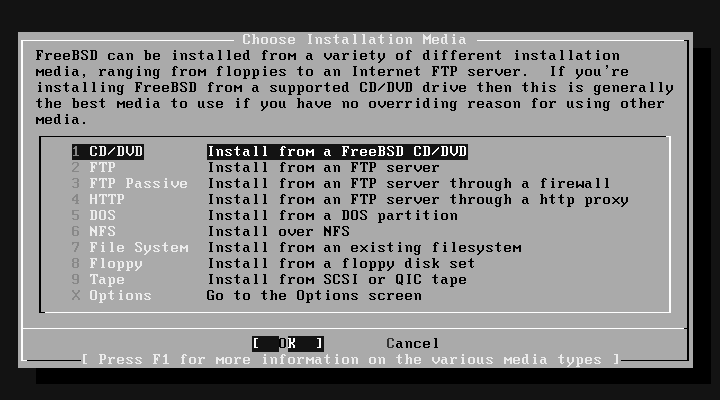
\includegraphics[width=6cm]{image200906/kfreebsd07_mono.png}
\end{minipage}

次はイントールメディアの選択 (Choose Installation Media) ですが、
ここでは必ず "1 CD/DVD" を選択してください。
その他の選択肢は FreeBSD のインストーラだったころの名残りです。
自分の環境にあわせ、"cd0" (SCSI) または "acd0" (ATAPI) を選べば、
インストールの始まりです。
途中で、"Alt-F3" を押すよう指示がありますから、それに従うと、
Debian GNU/Linux でお馴染みな、タイムゾーンの設定とか popularity-contest 
の設定とかができます。
Debian GNU/kFreeBSD 特有なものは、module-init-tools の設定で、
これは FreeBSD カーネルのモジュール名を選ばなければなりません。
ネットワークカードモジュールとサウンドカードモジュールとその他のモジュールが出てきますが、
詳しくは FreeBSD 本家のドキュメントを見てください。
私の場合は VMware ですので、サウンドカードモジュールの "snd\_es137x" のみ選びました。
\\
\begin{minipage}{0.4\hsize}
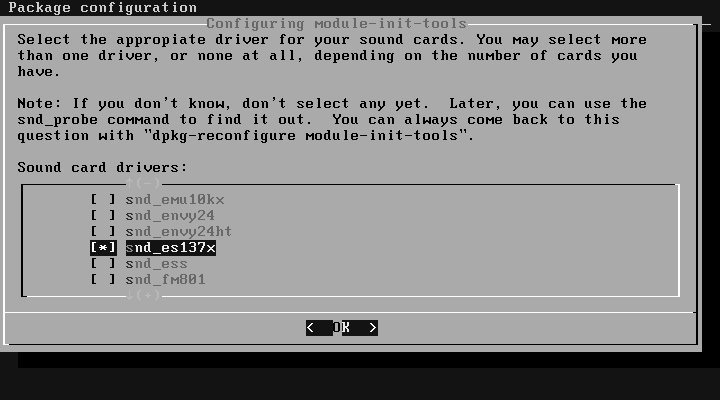
\includegraphics[width=6cm]{image200906/kfreebsd12_mono.png}
\end{minipage}
\begin{minipage}{0.4\hsize}
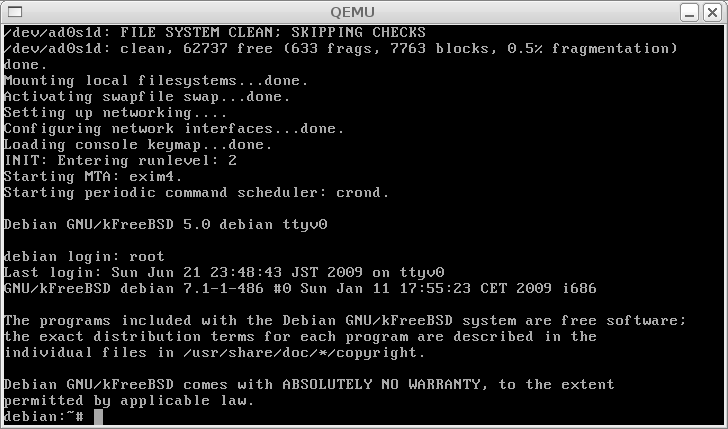
\includegraphics[width=6cm]{image200906/kfreebsdlogin_mono.png}
\end{minipage}

最初の画面に戻ってきたらインストールは終わりです。
タブキーで "X Exit Install" を選び、再起動して下さい。

最初は root ユーザのみがパスワード無しで出来ています。
ユーザ名 root を入力すると、パスワードをきかれずにログインできます。


root でログインしたら、まずはpasswdコマンドでパスワードを変更しましょう。
\begin{commandline}
passwd
\end{commandline}

次にネットワークの接続をします。
Linux の eth0 にあたるものは le0 (VMware の場合) または ed0 (Qemu の場合) 
のようです。
dhcp3-client パッケージは既にインストール済みのはずですから、DHCP 環境
\footnote{qemu の場合デフォルトでは dhcp でIPアドレスが取得できます}の人は /etc/network/interfaces を編集しなくても
\begin{commandline}
# dhclient3
\end{commandline}
でネットワークに繋がるはずです。

固定 IP の人は、以下を参考にして、それぞれのファイルを編集して下さい。
\begin{commandline}
##/etc/network/interfaces の例
auto lo0
iface lo0 inet loopback
## Static network
auto le0
iface le0 inet static
    address 192.168.0.3
    network 192.168.0.0
    netmask 255.255.255.0
    gateway 192.168.0.1
\end{commandline}
\begin{commandline}
##/etc/resolv.conf の例
nameserver 192.168.0.1
\end{commandline}
その後、
\begin{commandline}
# ifup le0
\end{commandline}
で、ネットワークに繋いで下さい。

インターネットに繋がったら、まず keymap の設定のため、
\begin{commandline}
# apt-get update
# apt-get install kbdcontrol
\end{commandline}
をして、console の keymap を選んでください。(console-data は使えません)

インストール後は、Debian GNU/Linux とどこが違うのか分からない程、まさに Debian です。

\subsection{参考文献}

\begin{itemize}
 \item Installing Debian GNU/kFreeBSD
       \url{http://glibc-bsd.alioth.debian.org/doc/}: インストール方法が
       詳しく記載されています。
\end{itemize}

\dancersection{【CD/DVD/USBメモリ】Debian JP版 Debian Liveを作るよ【netbootも】}{のがたじゅん}
\index{Debian Live}
\index{USBめもりぶーと@USBメモリブート}
\index{CDぶーと@CDブート}

\subsection{はじめに}
OSをハードディスクにインストールせずメディアから直接起動して使う「ライブ
システム」が知られて久しいですが、DebianにもDebian Liveというライブシス
テムがあります。
今回はDebian Live作成ツールのlive-helperを使って、Debian JP版Debian Liveや
関西Debian勉強会の配布DVDを作成する中で、自分好みのDebianライブシステム
を作成する方法やコツなどを解説します。

\subsection{Debian Live Projectとは}
Debian Liveの作成の前に、Debian Live Projectについて紹介します。

Debian Live Projectは、ライブシステム作成のためのフレームワークlive-helperと
live-initramfsなどのライブシステムにまつわるユーティリティを開発するプロ
ジェクトで、Debianの公式サブプロジェクトです。

既存のライブシステム・ディストリビューションとの違いは、ライブシステムを
作ってリリースすることより、フレームワークとしてのツールの制作に重きを置
いているところでしょうか。

live-helperを使って作られたDebianライブシステムはDebian Liveと呼ばれ、Lennyから同時にリリースされています。

\subsection{Debian Liveの特徴}
Debian Liveは、既存のライブシステム・ディストリビューションの欠点を解消するように作られており、以下の特徴を持っています。

\begin{itemize}
 \item 一つのディストリビューションのみで完結。
 \item カーネルも含めてパッチを当てたりなど特別なパッケージを使わない。
 \item リマスタリングではない新しい環境からシステムを作ることができる。
 \item CD、DVD、USBメモリ起動のシステムだけでなく、ネットワークやインターネット越しに起動するシステムを作ることができる。
 \item 複数のアーキテキクチャをサポート。
 \item Debian Installerを含めることができる。
\end{itemize}

Debian LiveはDebianのみで作成できるようにデザインされていますが、自作のパッケージや独自のAptリポジトリのパッケージを追加して作ることも可能です。

アーキテキクチャについては、現在、正式に対応しているのはi386、amd64、
powerpcだけですが、基本的にDebianがサポートしているアーキテキクチャには
対応する予定です。サポートしているモードもDebianだけでなく、emdebianや
ubuntuにも対応しています。(sid以上で --mode
ubuntu と指定すると不完全ながらもubuntu liveができます。)
\index{ubuntu live}

Debian Installerについては通常のnetinstやbusinesscardのインストーラに加え、Debian Liveのパッケージをそっくりそのままインストールするliveもサポートされています。また、計画段階ですが、Debian Live上から直接Debianをインストールするためのインストーラの制作も予定されています。

\subsection{live-helperについて}
live-helperとは、Debian Liveを作成するためのファイル名の頭に「lh\_」とつ
いたシェルスクリプト群です。群というだけあってスクリプトは多数ありますが、
この中でDebian Live作成に使用するコマンドはたった3つ。設定のための
「lh\_config」、作成のための「lh\_build」、作業ディレクトリをクリーンナッ
プする「lh\_clean」だけです。
\index{live-helper}

残りのスクリプトは、3つのスクリプトの中から設定に応じて適宜呼ばれるので、
通常、意識する必要はありません。

\subsection{Debian Liveの最初の一歩}
それではlive-helperを使ったDebian Liveの作成の基本について解説します。

\subsubsection{live-helperのインストール}
live-helperは、すでにDebianのリポジトリに用意されているので、aptitudeなどを使ってインストールします。
パッケージインストールについての注意ですが、live-helperパッケージに
SuggestsやRecommendsされたパッケージを使用する場面が多いので、特に事情が無ければ、すべてインストールしておいてください。

live-helperのインストール
\begin{commandline}
# aptitude --with-recommends install live-helper
\end{commandline}

\subsubsection{作業の準備}
Debian Live作成のための作業ディレクトリを作成します。ここではlive-workと名づけて作りました。

 作業ディレクトリの作成
\begin{commandline}
$ mkdir live-work
\end{commandline}

Debian Liveの設定ファイルや作成作業のファイルは、すべてカレントディレクトリに置かれます。よく使うディレクトリでDebian Live作成作業をおこなうと、これらのファイルと通常のファイルが混ざって収集がつかなくなるので、作業の前には専用のディレクトリを用意しましょう。

\newpage

\subsubsection{まずDebian Liveを作ってみる}
設定にはlh\_configコマンドを使います。作業ディレクトリに降りてlh\_configと入力します。

\begin{commandline}
$ cd debian-live/
$ lh_config
\end{commandline}

configとscriptsディレクトリが作成されたはずです。ディレクトリの意味につ
いては後ほど説明するので、まずはDebian Liveを作成してみましょう。
「sudo lh\_build」と入力します。(lh\_configコマンド以外は管理者権限が必要になるので、コマンドの前にsudoをつけて実行します。)

\begin{commandline}
$ sudo lh_build
\end{commandline}

マシンとネットワークの状況にもよりますが15分〜30分ほどでbinary.iso、
binary.list、binary.packageというファイルができているはずです。他
にはbinary、cache、chrootというディレクトリができています。

できていなければ「sudo lh\_clean」と入力し、作業途中のディレクトリを消去してから、もう一度試してみてください。

\begin{commandline}
$ ls -la
drwxr-xr-x  6 jun  jun        296 2009-06-24 16:24 .
drwxr-xr-x 10 jun  jun        320 2009-06-24 16:08 ..
drwxr-xr-x  2 root root       640 2009-06-24 16:24 .stage
drwxr-xr-x  6 root root       176 2009-06-24 16:24 binary
-rw-r--r--  1 root root 132192256 2009-06-24 16:24 binary.iso
-rw-r--r--  1 root root      2171 2009-06-24 16:24 binary.list
-rw-r--r--  1 root root     11123 2009-06-24 16:23 binary.packages
drwxr-xr-x  6 root root       184 2009-06-24 16:08 cache
drwxr-xr-x 20 root root       600 2009-06-24 16:24 chroot
drwxr-xr-x 22 jun  jun        936 2009-06-24 16:08 config
\end{commandline}

\subsubsection{イメージファイルを確認する}
生成されたファイルの中にbinary.isoというファイルがあります。これがDebian LiveのCDイメージファイルです。
それでは起動テストをおこないますが、CD-Rなどに書き込んでのテストはマシン
を再起動しなければいけませんし、ライトワンスのメディアを使うのは環境にも
良くないので、仮想マシンを使って確認します。

例ではqemuを使いましたが、KVMやVirtualBox、VMware Playerなど好きな仮想化ソフトを使ってかまいません。qemuを使う場合、そのままの状態では遅いので、あらかじめ高速化カーネルモジュールのkqemuを組み込んでおいてください。

kqemuを組み込む
\begin{commandline}
# m-a a-i kqemu
# modprobe kqemu
\end{commandline}

qemu上でDebian Liveを実行する
\begin{commandline}
$ qemu -cdrom binary.iso -boot d -m 256
\end{commandline}

qemu上でDebian Liveが起動したでしょうか?画面は白黒のコンソール画面、キーボードは英語配列。想像していたものと、だいぶかけ離れた画面が現れたと思います。

これが最小のDebian Liveです。ここから自分なりの設定を加えて、自分オリジナルのDebian Liveを作り上げます。

\newpage

\subsection{Debian Liveの設定}
さて、これから本格的なDebian Liveの設定に入りますが、Debian Liveが作成される手順を知っておくと、より的確に設定することができるので説明します。

Debian Liveの作成にはlh\_buildコマンドを使いますが、lh\_buildは4つのコマ
ンドを呼び出しそれぞれの作業をおこないます。その4つのコマンドは以下になります。

\begin{enumerate}
 \item debootstrapによるベースシステムのインストール (lh\_bootstrap)
 \item ベースシステムにchrootして必要なソフトのインストールや設定をおこなう(lh\_chroot)
 \item 作成されたシステムを一つのファイルにまとめ、起動できるバイナリイメージを作成 (lh\_binary)
 \item 作成されたバイナリイメージにソースが必要ならば、ソースをまとめたイメージを作成 (lh\_source)
\end{enumerate}

このようにbootstrap→chroot→binary→sourceの順に作業が進み、それぞれのステージにおいて独自の設定をすることができます。

設定ファイルはconfigディレクトリ以下にありますが、common、bootstrap、
chroot、binary、sourceの5つのファイルはlh\_configから設定するので、直接
編集しません。

それ以外のディレクトリでは、chrootステージに関係したものは「chroot\_」、
binaryステージに関係したものは「binary\_」と、それぞれの状態を表すプリフィ
クスがついているので、参考にしながら場面に応じた設定をしていきます。

\subsubsection{設定と作成の基本}
Debian Liveの設定はlh\_configコマンドを使って行います。lh\_config --helpと入力してみましょう。

\begin{commandline}
$ lh_config --help
\end{commandline}

ものすごい数の設定が出てきましたが、すべてを設定する必要はありません。設定をしなければ基本の設定が使われるので必要な箇所のみ変更していきます。

\begin{commandline}
$ lh_config \
        --binary-images iso \
        --distribution lenny \
        --language ja \
        --bootappend-live "quiet locale=ja_JP.UTF-8 keyb=jp kmodel=jp106" \
        --mirror-bootstrap "http://ftp.jp.debian.org/debian/" \
        --mirror-chroot "http://ftp.jp.debian.org/debian/" \
        --mirror-chroot-security "http://security.debian.org/" \
        --mirror-binary "http://ftp.jp.debian.org/debian/" \
        --mirror-binary-security "http://security.debian.org/"
\end{commandline}

上から順に説明します。

--binary-imagesは生成するバイナリイメージの種類を指定します。iso以外にもusb-hddなど指定できます。--distributionにはディストリビューションを指定。lennyを指定しています。squeezeは現在カーネルパッケージの不整合があるので作れません。--languageは言語です。IceweaselやOpenOffice.orgのように言語別パッケージがあるときの判断に利用されます。

--bootappend-liveはDebian Live起動時のブートパラメータを指定します。ここ
  ではカーネルのメッセージ出力を抑制する「quiet」と、ロケールとキーボードを日本語の設定にしています。quiet以外はDebian Live独自のパラメータです。パラメータ一覧は、live-initramfsパッケージの/usr/share/doc/live-initramfs/parameters.txtを参照してください。

--mirrorはAptの取得先を指定します。ミラーは、それぞれのステージで設定で
  きますが、特別な事がない限り分けて指定する必要はないので、ftp.jp.debian.orgとsecurity.debian.orgを設定しています。

\newpage

とても長かったですが、これを毎回設定するのは大変です。
毎回設定しないようにするには、どうしたらいいのでしょうか。

lh\_configを最初に実行した際、設定を保存するconfigディレクトリのほかに、
scriptsディレクトリが生成されていたことを覚えているでしょうか。
そのscriptsディレクトリに設定のためのconfigをスクリプトとして置きましょう。

scripts/config

\begin{commandline}
#!/bin/sh

MIRROR_DEBIAN="http://ftp.jp.debian.org/debian/"
MIRROR_SECURITY="http://security.debian.org/"

BOOTOPTION_LIVE="quiet locale=ja_JP.UTF-8 keyb=jp kmodel=jp106"

lh_config noautoconfig \
        --binary-images iso \
        --distribution lenny \
        --language ja \
        --bootappend-live "${BOOTOPTION_LIVE}" \
        --mirror-bootstrap ${MIRROR_DEBIAN} \
        --mirror-chroot ${MIRROR_DEBIAN} \
        --mirror-chroot-security ${MIRROR_SECURITY} \
        --mirror-binary ${MIRROR_DEBIAN} \
        --mirror-binary-security ${MIRROR_SECURITY}
        ${@}
\end{commandline}


このscripts/configスクリプトは、lh\_configコマンドを実行したとき、scripts/configスクリプトが存在すれば、再帰的に呼び出され実行される仕組みになっています。

これを見て {\bf わざわざ手間のかかることをしているのはなぜ?}と思った方も
いると思います。それには{\bf クリーンな環境からのビルド}と{\bf ビルドの自動化}の二つの理由があります。

「クリーンな環境からのビルド」ですが、live-helperで生成した設定ファイルは
今は何も変わりませんが、この先バージョンが上がった場合どうでしょう?
オプションが廃止されたり、新しいオプションが追加されるかもしれません。
古いバージョンの設定ファイルを使いつづけていると、それらに気づかないまま
対応できない以外にも、無用なトラブルを呼び込むかもしれません。

それらを避けるためにも毎回configディレクトリを消去して新たに設定を生成す
る必要があります。

もう一つ {\bf ビルドの自動化}ですが、ライブシステムでは、同一内容で設定が少
し違うものが欲しいことがあります。たとえばCDイメージ版とUSBメモリ版など
です。

そのとき、毎回オプションを指定して作ることは効率が悪いので、共通する設定はスクリプト化しておき、変更点のみ指定して2回呼び出せば、クリーンかつ必要なイメージを作成することができます。

scripts/configスクリプトに続いて、lh\_buildコマンドから呼び出されるscripts/buildスクリプトと、lh\_cleanコマンドから呼び出されるscripts/cleanスクリプトも作っておきましょう。

scripts/buildスクリプトでは、ビルド作業のログと生成されるイメージをわかりやすくするためファイル名に作業時間を含めるようにし、scripts/cleanスクリプトは、configディレクトリ内で空のディレクトリも消去するようにしています。

scripts/build

\begin{commandline}
#!/bin/sh

IMAGE_PREFIX=debian_live-binary
BUILDDATE=`date +%Y%m%d%H%M%S`

lh_build noautoconfig 2>&1 | tee ${IMAGE_PREFIX}-${BUILDDATE}.buildlog

# rename files
if [ -f binary.iso ]; then
   mv binary.iso ${IMAGE_PREFIX}-${BUILDDATE}.iso
elif [ -f binary.img ]; then
   mv binary.img ${IMAGE_PREFIX}-${BUILDDATE}.img
fi
[ -f binary.list ] && mv binary.list ${IMAGE_PREFIX}-${BUILDDATE}.list
[ -f binary.packages ] && mv binary.packages ${IMAGE_PREFIX}-${BUILDDATE}.packages
\end{commandline}

\newpage

scripts/clean

\begin{commandline}
#!/bin/sh

lh_clean noautoconfig --all ${@}

# Remove generated files
rm -f config/binary config/bootstrap config/chroot config/common config/source

# Remove empty directories in config tree
if ls config/*/ > /dev/null 2>&1
then
    rmdir --ignore-fail-on-non-empty config/*/
fi

if [ -d config ]
then
    rmdir --ignore-fail-on-non-empty config
fi
\end{commandline}

これでlh\_configと入力すると、いつでも自分の基本設定の状態から作成すること
ができます。
sudo lh\_buildやsudo lh\_cleanと入力するとログをとりながらビルドしたり、
クリーンナップもできます。

さて、自動化といえばMake。ということで簡単ですがMakefileも用意してみまし
た。sudo lh\_buildなんて長く打たなくてもmakeと入力するだけでビルドできま
すし、ほんの少し設定を変えるときもMakefileの中で処理することができるので、とても楽になりました。

Makefile

\begin{commandline}
all: config build

config: clean
        lh_config

build:
        sudo lh_build

clean:
        sudo lh_clean

distclean: clean
        sudo lh_clean --purge
        sudo rm -f *.iso *.img *.list *.packages *.buildlog *.md5sum
\end{commandline}

もう一つついでに、gitでlive-helperのレシピを管理するととても楽ですが、そ
の場合、以下のような「.gitignore」を作成しておくとよいでしょう。

\begin{commandline}
*.buildlog
*.img
*.iso
*.list
*.md5sum
*.packages
*~
.*~
.stage/
binary/
cache/
chroot/
config/binary
config/bootstrap
config/chroot
config/common
config/source
\end{commandline}

\newpage

\subsection{Debian Liveのカスタマイズ}
作成環境ができあがったので、具体的なカスタマイズについて述べます。

\subsection{パッケージの追加}
自分好みのDebian Liveにするために最初に始めることはパッケージの追加でしょ
う。パッケージを追加するにはいくつか方法はありますが順番に説明します。

\subsubsection{パッケージを追加する}
APTリポジトリにあるパッケージを追加するには--packagesオプションを使います。パッケージの指定方法は、パッケージ名をスペースで区切って並べていきます。

\begin{commandline}
$ lh_config --packages "PACKAGE PACKAGE2 …"
\end{commandline}

自作パッケージを追加するには、config/chroot\_local-packages/ディレクトリにdebパッケージを置き、--packagesオプションでパッケージ名を指定します。

\subsubsection{パッケージリストで追加する}
--packagesオプションでは、まとまった数のパッケージを追加するには、いくつもパッケージ名を並べないといけないので不便です。
よく使われるデスクトップ環境などのパッケージリストはデフォルトで用意されているので、--packages-listsオプションを使って指定します。

パッケージリストの一覧は/usr/share/live-helper/lists/をご覧ください

\begin{commandline}
$$ lh_config --packages-lists "gnome"
\end{commandline}

自分で追加したいパッケージ名を並べたパッケージリストをconfig/chroot\_local-packageslists/ディレクトリに用意し、--packages-listsオプションで指定することもできます。

「FILE」という名前のパッケージリストを作成
\begin{commandline}
$ vi config/chroot_local-packageslists/FILE

$ cat  config/chroot_local-packageslists/FILE
lv manpages-ja nkf
iceweasel-l10n-ja
openoffice.org-help-ja openoffice.org-l10n-ja
ttf-kochi-gothic ttf-kochi-mincho ttf-sazanami-gothic ttf-sazanami-mincho ttf-vlgothic
uim uim-applet-gnome uim-prime uim-qt uim-qt3
\end{commandline}

--packages-listsオプションで「FILE」を指定します。
\begin{commandline}
$ lh_config --packages-lists "FILE"
\end{commandline}

\subsubsubsection{パッケージリスト書式}

別のパッケージリストを含める方法
\begin{commandline}
#include <gnome>
iceweasel
\end{commandline}

アーキテクチャで分岐する方法
\begin{commandline}
#if ARCHITECTURE amd64
ia32-libs
#endif
\end{commandline}

セクションで分岐する方法
\begin{commandline}
#if SECTIONS contrib non-free
vrms
#endif
\end{commandline}

\subsubsection{APTリポジトリを追加する}
APTリポジトリを追加するには、config/chroot\_sources/ディレクトリにApt-lineを書いたファイルと、パッケージの署名を検証するGPG鍵ファイルを置きます。

Apt-lineを書いたファイル名はchrootステージとbinaryステージで別々に指定す
ることができ、chrootステージの場合には拡張子を {\bf .chroot}、binaryステー
ジでは拡張子を {\bf .binary}にします。GPG鍵ファイルは拡張子を {\bf .gpg}にしておきます。

\begin{commandline}
restricted-debian_multimedia.chroot
restricted-debian_multimedia.chroot.gpg
restricted-debian_multimedia.binary
restricted-debian_multimedia.binary.gpg
\end{commandline}

\subsubsubsection{キーリングパッケージを指定する}
GPG鍵がキーリングパッケージとして配布されている場合は、--keyring-packagesオ
プションにキーリングパッケージを指定します。

\begin{commandline}
$ lh_config --keyring-packages "debian-archive-keyring debian-multimedia-keyring"
\end{commandline}

\subsubsection{ファイルを追加する}
パッケージではなく、ファイルそのものを追加する場合はconfig/chroot\_local-includes/ディレクトリにファイルを置きます。
ファイルを置く場合の注意としては、ディレクトリ構造がそのままコピーされる
ので、/usr/local/bin/hogeというファイルを置く場合は、
config/chroot\_local-includes/ディレクトリをトップに見立てusr/local/bin/ディレクトリを作り、その中にhogeを置きます。

/usr/local/bin/hogeを置く場合のディレクトリ構造
\begin{commandline}
$ ls chroot_local-includes/usr/local/bin/
hoge
\end{commandline}

\subsubsection{カーネルパッケージを追加する}
カーネルパッケージを指定してインストールするには、--linux-packagesオプションと--linux-flavoursオプションを設定します。

\begin{commandline}
$ lh_config --linux-packages "linux-image-2.6 aufs-modules-2.6 squashfs-modules-2.6" --linux-flavours "686"
\end{commandline} 

\subsubsubsection{カスタムカーネルパッケージを追加する}
カスタムカーネルパッケージを追加するには、カーネルのパッケージ以外にも、ファイルシステムを透過的に重ねるaufs/unionfsパッケージ、Kernel 2.6.28以前のカーネルでsquashfsを使うならsquashfsパッケージなどを用意する必要があります。

\begin{enumerate}
 \item 用意したパッケージをconfig/chroot\_local-packages/ディレクトリに置く。
 \item --linux-packagesオプションに"none"、--linux-packagesオプションに用意したパッケージそれぞれを書く。--linux-flavoursオプションにはパッケージ名のカーネルバージョン以降を書く。
\end{enumerate}

\begin{commandline}
$ lh_config --linux-packages "none" --linux-packages \
  "linux-image-2.6.26.6-rt11 aufs-modules-2.6.26.6-rt11 squashfs-modules-2.6.26.6-rt11" --linux-flavours "rt11"
\end{commandline}

\subsection{設定のカスタマイズ}
パッケージを追加したなら、次は設定を追加しましょう。
設定の追加にもさまざまなパターンがあるので、順に紹介します。

\subsubsection{シェルスクリプトを実行する}
Debian Liveで設定変更のため一番使われる手法は、シェルスクリプトを実行す
ることです。パッケージのインストールから設定の書き換え、不要ファイルの除去など、ほぼなんでも行うことができます。

シェルスクリプトを実行するには、config/chroot\_local-hooks/ディレクトリに実行させたいシェルスクリプトを置きます。

スクリプト例(Iceweaselの初期設定を変更する)
\begin{commandline}
#!/bin/bash
set -e

ICEWEASEL_PREFS=/etc/iceweasel/profile/prefs.js

cat << _EOL_ >>${ICEWEASEL_PREFS}

/* Debian Live tune */
user_pref("browser.cache.disk.parent_directory","/tmp");
user_pref("browser.cache.disk.capacity", 5000);
user_pref("browser.startup.homepage", "http://www.debian.or.jp/");
_EOL_
\end{commandline}

\subsubsection{パッチを当てる}
設定の変更にはシェルスクリプトを実行してsedで書き換えてもいいですが、パッチを当てたほうが早い場合もあります。
パッチを当てるにはchrootのトップからpatch -p1で当てられるように作ったパッチファイルをconfig/chroot\_local-patches/ディレクトリに置きます。

パッチファイル例(/etc/dhcp3/dhclient.confを変更する)
\begin{commandline}
*** chroot/etc/dhcp3/dhclient.conf.orig 2009-04-12 23:03:36.000000000 +0900
--- chroot/etc/dhcp3/dhclient.conf      2009-04-12 23:05:05.000000000 +0900
***************
*** 23,30 ****
       netbios-name-servers, netbios-scope, interface-mtu,
       rfc3442-classless-static-routes;
 #require subnet-mask, domain-name-servers;
! #timeout 60;
! #retry 60;
 #reboot 10;
 #select-timeout 5;
 #initial-interval 2;
--- 23,30 ----
       netbios-name-servers, netbios-scope, interface-mtu,
       rfc3442-classless-static-routes;
 #require subnet-mask, domain-name-servers;
! timeout 0;
! retry 0;
 #reboot 10;
 #select-timeout 5;
 #initial-interval 2;
\end{commandline}

\subsubsection{debconfの設定をする}
/etcにある設定などはシェルスクリプトやパッチで書き換えることができますが、
debconfの設定はdbに納めれられているので直接書き換えることはできません。
その場合はconfig/chroot\_local-preseed/ディレクトリにdebconfの設定を置い
て設定します。
debconfの設定は、debconf-utilsパッケージに納められているdeboconf-get-selectionsを使って読み出します。

\newpage

FUSE(Filesystem in Userspace)を使うためにユーザーをfuseグループに登録するには

\begin{enumerate}
 \item debconfの設定を取り出してconfig/chroot\_local-preseed/user-default-groups.preseedに書き出す
 \begin{commandline}
$ sudo debconf-get-selections | grep user-default-groups > config/chroot_local-preseed/user-default-groups.preseed 
 \end{commandline}
 \item fuseグループを追加
 \begin{commandline}
user-setup      passwd/user-default-groups      string  audio cdrom dialout floppy video plugdev netdev powerdev scanner fuse
 \end{commandline}
\end{enumerate}

\subsubsection{ブートローダーについて}
ブートローダーについてはi386/amd64ではsyslinuxとgrubが選択できます。

ブートローダーのスプラッシュ画面を変更するには、syslinuxの場合はconfig/binary\_syslinux/ディレクトリに、grubの場合はconfig/binary\_grub/ディレクトリに設定を置きます。

grubについてですが、usb-hddではgrubのインストールがまだサポートされていないので、syslinuxしか使うことができません。誰か書いてみませんか?

\subsubsection{スプラッシュスクリーンについて}
最近のディストリビューションは起動時にスプラッシュスクリーンを表示していますが、Debian Liveでも可能です。splashyかusplashパッケージをインストールして、--bootappend-liveオプションに"vga=788 splash"と加えてください。vgaの部分はフレームバッファの解像度なので適宜変更してください。

\subsubsection{作成されるファイルとディレクトリについて}

lh\_configやlh\_buildが作成するファイルとディレクトリは以下のようになります。

\begin{table}[htbp]
\caption{Debian Liveのディレクトリ}
\begin{tabular}{|l|l|}
\hline
.stage/ & 進行状況を示すフラグが納められる \\ \hline
config/ & 設定が納められる \\ \hline
scripts/ & 作成のためのconfig、build、cleanスクリプトを置く \\ \hline
cache/ & パッケージなどをキャッシュされる \\ \hline
chroot/ & chrootイメージの作業ディレクトリ \\ \hline
binary/ & binaryイメージの作業ディレクトリ \\ \hline
\end{tabular}
\label{}
\end{table}

\subsection{その他、積み残したことなど}

\subsubsection{Debian Liveを使っていてデータを保存するには}
出来上がったDebian Liveを使っていて、データを保存しておきたいことがあり
ます。

その場合は、全体を保存するにはlive-rw、ホームディレクトリのみを保存するな
らhome-rwというラベル名で、ext2/3でフォーマットしたパーティションをあらか
じめ作成しておき、起動時、ブートパラメータにpersistentをつけて起動すると
自動的にそれぞれのパーティションをマウントします。

専用パーティションを用意しない場合は、live-snapshotコマンドを使うとデー
タが保存できるようなのですが、persistentをつけてもなぜか読み込んでくれないので、誰かlive-snapshotの使い方を知っていたら教えてください。

\newpage

\subsubsection{live-helperとDebian Live関連パッケージ}
Debian Live関連するパッケージについては以下のようになります。

Debian公式パッケージ
\begin{itemize}
 \item live-helper: Debian Liveを作成するためのスクリプト。
 \item live-initramfs: Debian Liveが起動する際に使われるinitramfsの中で動くスクリプト。
 \item live-magic: GUIでDebian Liveを作成するプログラム。決まったものしかできないので使うことないと思います。
\end{itemize}

Debian Live Projectのみで配布(Debian非公式パッケージ)
\begin{itemize}
 \item live-manual: マニュアル
 \item live-initscripts: 起動時にスクリプトを実行するオプションを追加する
 \item live-helper, live-initramfs, live-magicのスナップショット
\end{itemize}

Debian Liveの開発はとても早いので、興味があるなら、Debian Live Projectで配布されているスナップショット版かgitのものを使うとよいでしょう。
スナップショットの在り処などは、Debian Live Projectのリンクページ\footnote{\url{Debian Live Project: http://debian-live.alioth.debian.org/links.html}}に掲載されています。

live-helperはDebianに依存しないように作られています。Debian以外のシステムでも以下の要件を満たしていれば、live-helperを使ってDebian Liveを作成することができます。

\begin{itemize}
 \item Linux 2.6.x
 \item POSIX準拠のシェル(bashやdashなど)
 \item 管理者(root)権限
 \item debootstrapもしくはcdebootstrap
 \item live-helper
\end{itemize}

\subsection{まとめ}
Debian Liveを使っていて、日本語のまとまった資料があまりないので頑張って書いてみましたが、いかがでしたでしょうか?
今回はCD/DVD/USBメモリ起動に絞って書きましたが、ネットワーク越しのブートや、live-helperの構造など、まだまだ書ききれない部分が残っているので、それはまた日を改めてということで、皆様のお役に立てればさいわいです。

\newpage

% \subsection{参考資料}
\begin{thebibliography}{99}
 \bibitem{Debian Live Project}
	 Debian Live Project: \url{http://debian-live.alioth.debian.org/}
 \bibitem{DebianLive}
	 DebianLive - Debian Wiki: \url{http://wiki.debian.org/DebianLive}
 \bibitem{DebianLive/FAQ}
 	 DebianLive/FAQ - Debian Wiki: \url{http://wiki.debian.org/DebianLive/FAQ}
 \bibitem{Debian Live Manual}
	 Debian Live Manual: \url{http://live.debian.net/manual/html/index.html}
 \bibitem{Daniel Baumann}
	 Daniel Baumann - Blog: Debian Live Initiative\\
	 \url{http://blog.daniel-baumann.ch/2006/02/14\#20060214_debian-live-initiative}
 \bibitem{tokyo34}
	 第34回東京エリアDebian勉強会、2007年11月勉強会:\\
	 \url{http://tokyodebian.alioth.debian.org/2007-11.html}
 \bibitem{softwaredesign200808}
	 Software Design 2008年8月号\\
	 live-helperで構築するオリジナルLive CD 岩松信洋
 \bibitem{softwaredesign200905}
	 Software Design 2009年5月号\\
	 インストール、ネットブック活用から独自バージョンの作成まで - Ubuntuの魅力を体感!\\
	 6章:Inside Ubuntu 吉田史\\
	 7章:カスタムCDイメージの作成 小林準
\end{thebibliography}

\dancersection{ハッカーに一歩近づく Tips:Bash 編}{山下康成@京都府向日市}
\index{bash}

\begin{table}[h]
\begin{center}
 \scriptsize
\caption{Bash コマンド一覧}
\begin{tabular}{|r|l|l|}
\hline
\multicolumn{3}{|c|}{<<コマンドの再実行>>}\\ \hline
1 & 以前実行したコマンドラインの呼出し &  上矢印キー、下矢印キー \\ \hline
2 & 以前実行したコマンドラインの呼出し & CTRL-P, CTRL-N \\ \hline
3 & 直前のコマンドの再実行 & !! \\ \hline
4 & 以前実行したコマンドラインに前方一致 & !(前方一致文字列) \\ \hline
5 & 以前実行したコマンドラインに部分一致 & !?(部分一致文字列) \\ \hline
6 & これまでに実行したコマンドラインの列挙 & history \\ \hline
7 & ヒストリ番号を用いた過去コマンド指定 & !(数字) \\ \hline
8 & 指定した回数前に実行したコマンド & !(負の数字) \\ \hline
9 & 実行されるコマンドの確認 & :p \\ \hline
\multicolumn{3}{|c|}{<<補完>>}\\ \hline
10 & パス名の補完 & TAB \\ \hline
11 & コマンドの補完 & TAB \\ \hline
\multicolumn{3}{|c|}{<<行編集>>}\\ \hline
12 & カーソルの左右移動 & CTRL-B/左矢印、CTRL-F/右矢印 \\ \hline
13 & カーソルの左の文字の消去 & BackSpace/Delete \\ \hline
14 & カーソルの行頭・行末への移動 & CTRL-A, CTRL-E \\ \hline
15 & カーソル位置の文字を消す & CTRL-D \\ \hline
16 & 行末まで消去 & CTRL-K \\ \hline
17 & 語頭まで消去 & CTRL-W \\ \hline
18 & 文字の入れ換え & CTRL-T \\ \hline
\multicolumn{3}{|c|}{<<直前のコマンドの一部を再利用する>>}\\ \hline
19 & 直前のコマンドの最後の引数 & !\$ \\ \hline
20 & 直前のコマンドの引数 & !* \\ \hline
21 & 直前のコマンドラインの一部を変更 & \^{ }A\^{ }B \\ \hline
22 & 直前のコマンドラインの一部を変更 & (以前のコマンド指定):s/A/B/ \\ \hline
\multicolumn{3}{|c|}{<<ワイルドカード>>}\\ \hline
23 & \.(ドット)で始まる以外に一致 & * \\ \hline
24 & 1文字に一致 & ? \\ \hline
\multicolumn{3}{|c|}{<<プログラムの実行結果を利用する>>}\\ \hline
25 & パイプ & \verb+|+ \\ \hline
26 & リダイレクト & $>$ $>>$ $<$ \\ \hline
27 & コマンドの実行結果を文字列として扱う & `(逆シングルクォート) \\ \hline
\multicolumn{3}{|c|}{<<その他>>}\\ \hline
28 & ホームディレクトリを指す & \verb+~+ \\ \hline
29 & 指定したユーザのホームディレクトリを指す & \verb+~+ユーザ名 \\ \hline
30 & (コマンドを中断する) & CTRL-C \\ \hline
\end{tabular}
\label{sonota} 
\end{center}
\end{table}

\subsection{参考資料}

\begin{itemize}
 \item ハッカーに一歩近づく Tips: Bash編\\
       \url{http://www.yamasita.jp/tips/bash/}
\end{itemize}

% 200911
\dancersection{Debianでの数学ことはじめ。}{まえだこうへい}
\index{GNU R}
\index{GNU Octave}
\index{Gnuplot}
% ===============================================================

\subsection{はじめに}

Debianで数値計算や統計処理、グラフ作成を行うには、様々なパッケージがあり
ます。私のように大学での専行が理系といっても基礎生物学だった人間には、コン
ピュータでの専用ツールでなくても、極端な話、基本的な統計学と関数電卓があ
れば事足りました。スプレッドシートを使っても、関数は使わずに電卓代わりに
使うことも多かったと記憶してます\footnote{理由は、当時のスプレッドシート
の関数の精度が低く、自分で計算式を作った方が確実だったためです。今では改
善されたのでしょうか?}。社会人になってからもその延長でスプレッドシート
で大抵は事足りる、という方が一般的には多いのではないかと思います。

とはいえ、数万単位のサンプル数の計算をしたり、グラフを描写する場合、スプレッ
ドシートでは非力だという問題もあります。プリセールスや企画で裏付け資料を
作るのにサンプルデータを統計処理したり、データをプロットしてグラフを描く
と、スプレッドシートだとマウスの操作だけで簡単にできる一方、CPUやメモリ
不足でレスポンスが遅くなったり、ソフトウェア自体が落ちたり、酷いとOS自体
のレスポンスも悪化するというのが最近の仕事上での悩みだったりします。

そんなことがきっかけで今頃、Gnuplotを使い始めたわけですが、統計処理では
最近はRの書籍を書店で見かけたり、数値計算ではOctaveというのがあると
いうことをDebian勉強会のMLで知ったり\footnote{RやOctaveのパッケージ
メンテナであるDirk Eddelbuettel さんが近々来日されるというのがMLで流れて
いたそもそものきっかけです。\url{http://dirk.eddelbuettel.com/}}と、自分
の中だけでなく、最近意外とまわりでもこの辺はホットな話題ではないかと思い
ます。そこで、今回は私と同じように入門者向けに Octave、Gnuplotとの連携方
法、Rの話に加え、Debianでの使い方、パッケージングなどについて説明しよう
と思います。


\subsection{概要}
GNU Ocatave は計算処理のための高級言語で、MATLABという数値計算の商用ソフ
トウェアとの互換性があるようです。行列計算、連立方程式、微分・積分、グラ
フ出力などに使えます。グラフ描画のためには、gnuplotが必要です。

一方、GNU Rは統計解析のためのプログラミング言語で、文法的には、S言語や
Schemeに影響を受けているようです。Octaveとは異なり、グラフ描画には
gnuplotは必要ないようです。Excelなどのデータ読み込みができるといった、デー
タの互換性にも特徴があります。


\subsection{インストール方法}

Debian での各実行環境の導入方法について見てみます。今回の前提条件として、
ディストリビューションは Sid\footnote{2009年11月10日現在。}としています
が、Stable(Lenny)や Testing(Squeeze)でもバージョンが異なることを除けばほ
ぼ同じです。適宜読み替えてください。

\subsubsection{Octaveのインストール方法}

GNU OctaveはSqueeze/Sidでは、\texttt{octave}というパッケージ名ではなく、
バージョン3.0と3.2で別のパッケージになっています。今回は3.2のパッケージ
を導入します。

\begin{commandline}
$ sudo apt-get install octave3.2
\end{commandline}

\subsubsection{GNU Rのインストール方法}

GNU Rは、Debianパッケージでの名前は、gnurでも、rでもgnu-rでもありません。
\texttt{r-base}というメタパッケージで提供されています。これをインストールすると、
最低限、\texttt{r-base-core}パッケージがGNU Rの実行には必要です。また、GNU Rには、
機能拡張のパッケージが用意されています。CRAN(the Comprehensive R Archive
Network)からダウンロードできます。Perlでの CPAN のような位置づけです。
千以上ものパッケージがあるようです。Debianでは、CPANや Ruby gemsと同様に
ここから直接ダウンロードすることもできますが、約150のRパッケージがdebパッ
ケージとして用意されています\footnote{2009年11月9日現在。}。パッケージ名
は''\texttt{r-cran-<name>}''というネーミングルールです。

今回は\texttt{r-base}をインストールしましたが、余計なパッケージを入れな
いようにと、\texttt{r-base-core}パッケージをインストールしたとしても最小
構成からのパッケージの差は二つしかありません。\footnote{一つは\texttt{r-base}, も
う一つは\texttt{r-base-dev}です。}

\begin{commandline}
$ sudo apt-get install r-base
\end{commandline}

\subsubsection{Gnuplotのインストール}

GnuplotはOctave、GNU Rのいずれもdebパッケージとしての依存関係はありませ
んが、octaveではgnuplotを使ってグラフ描画もできるので、インストールして
おくと便利でしょう。gnuplotのインストールには\texttt{gnuplot}パッケージ
をインストールします。

\begin{commandline}
$ sudo apt-get install gnuplot
\end{commandline}

\subsection{試してみる。}

今回は、我が家の過去9年分の光熱費における各使用量の分布をサンプルデータ
としてみます。まずは、もともと使い始めていた gnuplot での例をみて、それ
に対し、Octave, R ではどのように処理するのかを見てみましょう。

用意したサンプルデータは以下のようなものです。

\begin{commandline}
"date","days","kWh","kWh/d","yen/d","yen","days","m^3","m^3/d","yen/d","yen","days","m^3","m^3/d","yen/d","yen","yen/d","yen"
2001/04,11,34,3.09,83.5,918,36,4.9,0.14,108.3,3900,58,9,0.16,22.8,1320,,
2001/05,33,95,2.88,73.8,2434,29,3.5,0.12,114.1,3310,,,,,,,
2001/06,30,129,4.3,102.7,3082,32,3,0.09,96.9,3100,61,3,0.05,15.7,960,,
2001/07,28,155,5.54,131.3,3676,28,1.7,0.06,91.1,2550,,,,,,,
(snip)
\end{commandline}

左から、年月,電気使用日数,月の電気使用量(kWh),1日あたりの電気使用量,1日
あたりの電気代,月の電気代,ガス使用日数,月のガス使用量(立方メートル),1日
あたりのガス使用量,1日あたりのガス代,月のガス代,水道使用日数,水道使用量
(立方メートル),1日あたりの水道使用量,1日あたりの水道代,月の水道代,1日あ
たりの下水道代,月の下水道代、となっています。

\subsubsection{gnuplot の場合}

gnuplotでは、次のようなバッチファイルを用意します。2001年4月から 2009年8
月までの電気、ガス、水道の各使用量をそれぞれプロットします。また、Debian
勉強会資料用に、LaTeXで取り込めるように、図はEPS、文字列はLaTeXで出力す
るようにします。

\begin{commandline}
reset
set terminal epslatex input color
set output "gnuplot.tex"
set datafile separator ","
set xdata time
set timefmt "%Y/%m"
set format x "%Y/%m"
set xtics rotate by -90
set mxtics 12
set xrange ["2001/04":"2009/08"]
set yrange [0:400]
set xlabel "年月"
set ylabel "電気使用量 [kWh]"
set y2range [0:50]
set y2label "ガス・水道使用量 [立方メートル]"
set ytics nomirror
set y2tics
plot "kohnetsuhi.csv" using 1:3 axes x1y1 title "電気" with line,\
     "" using 1:8 axes x1y2 title "ガス" with line,\
     "" using 1:13 axes x1y2 title "水道" with line
\end{commandline}

このバッチファイルをLaTeXとEPSに変換します。バッチファイルをロードするに
は、対話モードでloadコマンドを実行します。

\begin{commandline}
$ gnuplot

	G N U P L O T
	Version 4.2 patchlevel 6 
	last modified Sep 2009
	System: Linux 2.6.31.3

	Copyright (C) 1986 - 1993, 1998, 2004, 2007 - 2009
	Thomas Williams, Colin Kelley and many others

	Type `help` to access the on-line reference manual.
	The gnuplot FAQ is available from http://www.gnuplot.info/faq/

	Send bug reports and suggestions to <http://sourceforge.net/projects/gnuplot>


Terminal type set to 'wxt'
gnuplot> load ``gnuplot.gp''
gnuplot> quit
\end{commandline}

これで、カレントディレクトリに gnuplot.texとgnuplot.epsファイルが出力さ
れます。gnuplot.tex は、LaTeX文書の中で以下のように記述して取り込みます。

\begin{commandline}
\usepackage{graphicx}

(snip)

\begin{figure}[thbp]
% GNUPLOT: LaTeX picture with Postscript
\begingroup
  \makeatletter
  \providecommand\color[2][]{%
    \GenericError{(gnuplot) \space\space\space\@spaces}{%
      Package color not loaded in conjunction with
      terminal option `colourtext'%
    }{See the gnuplot documentation for explanation.%
    }{Either use 'blacktext' in gnuplot or load the package
      color.sty in LaTeX.}%
    \renewcommand\color[2][]{}%
  }%
  \providecommand\includegraphics[2][]{%
    \GenericError{(gnuplot) \space\space\space\@spaces}{%
      Package graphicx or graphics not loaded%
    }{See the gnuplot documentation for explanation.%
    }{The gnuplot epslatex terminal needs graphicx.sty or graphics.sty.}%
    \renewcommand\includegraphics[2][]{}%
  }%
  \providecommand\rotatebox[2]{#2}%
  \@ifundefined{ifGPcolor}{%
    \newif\ifGPcolor
    \GPcolortrue
  }{}%
  \@ifundefined{ifGPblacktext}{%
    \newif\ifGPblacktext
    \GPblacktexttrue
  }{}%
  % define a \g@addto@macro without @ in the name:
  \let\gplgaddtomacro\g@addto@macro
  % define empty templates for all commands taking text:
  \gdef\gplbacktext{}%
  \gdef\gplfronttext{}%
  \makeatother
  \ifGPblacktext
    % no textcolor at all
    \def\colorrgb#1{}%
    \def\colorgray#1{}%
  \else
    % gray or color?
    \ifGPcolor
      \def\colorrgb#1{\color[rgb]{#1}}%
      \def\colorgray#1{\color[gray]{#1}}%
      \expandafter\def\csname LTw\endcsname{\color{white}}%
      \expandafter\def\csname LTb\endcsname{\color{black}}%
      \expandafter\def\csname LTa\endcsname{\color{black}}%
      \expandafter\def\csname LT0\endcsname{\color[rgb]{1,0,0}}%
      \expandafter\def\csname LT1\endcsname{\color[rgb]{0,1,0}}%
      \expandafter\def\csname LT2\endcsname{\color[rgb]{0,0,1}}%
      \expandafter\def\csname LT3\endcsname{\color[rgb]{1,0,1}}%
      \expandafter\def\csname LT4\endcsname{\color[rgb]{0,1,1}}%
      \expandafter\def\csname LT5\endcsname{\color[rgb]{1,1,0}}%
      \expandafter\def\csname LT6\endcsname{\color[rgb]{0,0,0}}%
      \expandafter\def\csname LT7\endcsname{\color[rgb]{1,0.3,0}}%
      \expandafter\def\csname LT8\endcsname{\color[rgb]{0.5,0.5,0.5}}%
    \else
      % gray
      \def\colorrgb#1{\color{black}}%
      \def\colorgray#1{\color[gray]{#1}}%
      \expandafter\def\csname LTw\endcsname{\color{white}}%
      \expandafter\def\csname LTb\endcsname{\color{black}}%
      \expandafter\def\csname LTa\endcsname{\color{black}}%
      \expandafter\def\csname LT0\endcsname{\color{black}}%
      \expandafter\def\csname LT1\endcsname{\color{black}}%
      \expandafter\def\csname LT2\endcsname{\color{black}}%
      \expandafter\def\csname LT3\endcsname{\color{black}}%
      \expandafter\def\csname LT4\endcsname{\color{black}}%
      \expandafter\def\csname LT5\endcsname{\color{black}}%
      \expandafter\def\csname LT6\endcsname{\color{black}}%
      \expandafter\def\csname LT7\endcsname{\color{black}}%
      \expandafter\def\csname LT8\endcsname{\color{black}}%
    \fi
  \fi
  \setlength{\unitlength}{0.0500bp}%
  \begin{picture}(7200.00,5040.00)%
    \gplgaddtomacro\gplbacktext{%
      \csname LTb\endcsname%
      \put(1210,1408){\makebox(0,0)[r]{\strut{} 0}}%
      \put(1210,1829){\makebox(0,0)[r]{\strut{} 50}}%
      \put(1210,2250){\makebox(0,0)[r]{\strut{} 100}}%
      \put(1210,2671){\makebox(0,0)[r]{\strut{} 150}}%
      \put(1210,3092){\makebox(0,0)[r]{\strut{} 200}}%
      \put(1210,3513){\makebox(0,0)[r]{\strut{} 250}}%
      \put(1210,3934){\makebox(0,0)[r]{\strut{} 300}}%
      \put(1210,4355){\makebox(0,0)[r]{\strut{} 350}}%
      \put(1210,4776){\makebox(0,0)[r]{\strut{} 400}}%
      \put(1763,1276){\rotatebox{-90}{\makebox(0,0)[l]{\strut{}2002/01}}}%
      \put(2320,1276){\rotatebox{-90}{\makebox(0,0)[l]{\strut{}2003/01}}}%
      \put(2877,1276){\rotatebox{-90}{\makebox(0,0)[l]{\strut{}2004/01}}}%
      \put(3436,1276){\rotatebox{-90}{\makebox(0,0)[l]{\strut{}2005/01}}}%
      \put(3994,1276){\rotatebox{-90}{\makebox(0,0)[l]{\strut{}2006/01}}}%
      \put(4551,1276){\rotatebox{-90}{\makebox(0,0)[l]{\strut{}2007/01}}}%
      \put(5107,1276){\rotatebox{-90}{\makebox(0,0)[l]{\strut{}2008/01}}}%
      \put(5667,1276){\rotatebox{-90}{\makebox(0,0)[l]{\strut{}2009/01}}}%
      \put(6122,1408){\makebox(0,0)[l]{\strut{} 0}}%
      \put(6122,2082){\makebox(0,0)[l]{\strut{} 10}}%
      \put(6122,2755){\makebox(0,0)[l]{\strut{} 20}}%
      \put(6122,3429){\makebox(0,0)[l]{\strut{} 30}}%
      \put(6122,4102){\makebox(0,0)[l]{\strut{} 40}}%
      \put(6122,4776){\makebox(0,0)[l]{\strut{} 50}}%
      \put(440,3092){\rotatebox{90}{\makebox(0,0){\strut{}$BEE5$;HMQNL(B [kWh]}}}%
      \put(6759,3092){\rotatebox{90}{\makebox(0,0){\strut{}$B%,%9!&?eF;;HMQNL(B [$BN)J}%a!<%H%k(B]}}}%
      \put(3666,154){\makebox(0,0){\strut{}$BG/7n(B}}%
    }%
    \gplgaddtomacro\gplfronttext{%
      \csname LTb\endcsname%
      \put(5003,4603){\makebox(0,0)[r]{\strut{}$BEE5$(B}}%
      \csname LTb\endcsname%
      \put(5003,4383){\makebox(0,0)[r]{\strut{}$B%,%9(B}}%
      \csname LTb\endcsname%
      \put(5003,4163){\makebox(0,0)[r]{\strut{}$B?eF;(B}}%
    }%
    \gplbacktext
    \put(0,0){\includegraphics{image200911/gnuplot.eps}}%
    \gplfronttext
  \end{picture}%
\endgroup

\end{figure}
\end{commandline}

ただし、このままでは make が通りません。gnuplot.tex を書き換える必要があ
ります。次のように下から3行目の includegraphicsのパスを変更する必要があ
ります。

\begin{commandline}

$ diff -u gnuplot.tex.bk gnuplot.tex
--- gnuplot.tex.orig	2009-11-12 23:38:36.000000000 +0900
+++ gnuplot.tex	2009-11-12 23:39:39.000000000 +0900
@@ -111,7 +111,7 @@
       \put(5003,4163){\makebox(0,0)[r]{\strut{}水道}}%
     }%
     \gplbacktext
-    \put(0,0){\includegraphics{gnuplot}}%
+    \put(0,0){\includegraphics{image200911/gnuplot.eps}}%
     \gplfronttext
   \end{picture}%
 \endgroup
\end{document}
\end{commandline}

これで make すると、以下のような図を表示できます。

\begin{figure}[thbp]
 % GNUPLOT: LaTeX picture with Postscript
\begingroup
  \makeatletter
  \providecommand\color[2][]{%
    \GenericError{(gnuplot) \space\space\space\@spaces}{%
      Package color not loaded in conjunction with
      terminal option `colourtext'%
    }{See the gnuplot documentation for explanation.%
    }{Either use 'blacktext' in gnuplot or load the package
      color.sty in LaTeX.}%
    \renewcommand\color[2][]{}%
  }%
  \providecommand\includegraphics[2][]{%
    \GenericError{(gnuplot) \space\space\space\@spaces}{%
      Package graphicx or graphics not loaded%
    }{See the gnuplot documentation for explanation.%
    }{The gnuplot epslatex terminal needs graphicx.sty or graphics.sty.}%
    \renewcommand\includegraphics[2][]{}%
  }%
  \providecommand\rotatebox[2]{#2}%
  \@ifundefined{ifGPcolor}{%
    \newif\ifGPcolor
    \GPcolortrue
  }{}%
  \@ifundefined{ifGPblacktext}{%
    \newif\ifGPblacktext
    \GPblacktexttrue
  }{}%
  % define a \g@addto@macro without @ in the name:
  \let\gplgaddtomacro\g@addto@macro
  % define empty templates for all commands taking text:
  \gdef\gplbacktext{}%
  \gdef\gplfronttext{}%
  \makeatother
  \ifGPblacktext
    % no textcolor at all
    \def\colorrgb#1{}%
    \def\colorgray#1{}%
  \else
    % gray or color?
    \ifGPcolor
      \def\colorrgb#1{\color[rgb]{#1}}%
      \def\colorgray#1{\color[gray]{#1}}%
      \expandafter\def\csname LTw\endcsname{\color{white}}%
      \expandafter\def\csname LTb\endcsname{\color{black}}%
      \expandafter\def\csname LTa\endcsname{\color{black}}%
      \expandafter\def\csname LT0\endcsname{\color[rgb]{1,0,0}}%
      \expandafter\def\csname LT1\endcsname{\color[rgb]{0,1,0}}%
      \expandafter\def\csname LT2\endcsname{\color[rgb]{0,0,1}}%
      \expandafter\def\csname LT3\endcsname{\color[rgb]{1,0,1}}%
      \expandafter\def\csname LT4\endcsname{\color[rgb]{0,1,1}}%
      \expandafter\def\csname LT5\endcsname{\color[rgb]{1,1,0}}%
      \expandafter\def\csname LT6\endcsname{\color[rgb]{0,0,0}}%
      \expandafter\def\csname LT7\endcsname{\color[rgb]{1,0.3,0}}%
      \expandafter\def\csname LT8\endcsname{\color[rgb]{0.5,0.5,0.5}}%
    \else
      % gray
      \def\colorrgb#1{\color{black}}%
      \def\colorgray#1{\color[gray]{#1}}%
      \expandafter\def\csname LTw\endcsname{\color{white}}%
      \expandafter\def\csname LTb\endcsname{\color{black}}%
      \expandafter\def\csname LTa\endcsname{\color{black}}%
      \expandafter\def\csname LT0\endcsname{\color{black}}%
      \expandafter\def\csname LT1\endcsname{\color{black}}%
      \expandafter\def\csname LT2\endcsname{\color{black}}%
      \expandafter\def\csname LT3\endcsname{\color{black}}%
      \expandafter\def\csname LT4\endcsname{\color{black}}%
      \expandafter\def\csname LT5\endcsname{\color{black}}%
      \expandafter\def\csname LT6\endcsname{\color{black}}%
      \expandafter\def\csname LT7\endcsname{\color{black}}%
      \expandafter\def\csname LT8\endcsname{\color{black}}%
    \fi
  \fi
  \setlength{\unitlength}{0.0500bp}%
  \begin{picture}(7200.00,5040.00)%
    \gplgaddtomacro\gplbacktext{%
      \csname LTb\endcsname%
      \put(1210,1408){\makebox(0,0)[r]{\strut{} 0}}%
      \put(1210,1829){\makebox(0,0)[r]{\strut{} 50}}%
      \put(1210,2250){\makebox(0,0)[r]{\strut{} 100}}%
      \put(1210,2671){\makebox(0,0)[r]{\strut{} 150}}%
      \put(1210,3092){\makebox(0,0)[r]{\strut{} 200}}%
      \put(1210,3513){\makebox(0,0)[r]{\strut{} 250}}%
      \put(1210,3934){\makebox(0,0)[r]{\strut{} 300}}%
      \put(1210,4355){\makebox(0,0)[r]{\strut{} 350}}%
      \put(1210,4776){\makebox(0,0)[r]{\strut{} 400}}%
      \put(1763,1276){\rotatebox{-90}{\makebox(0,0)[l]{\strut{}2002/01}}}%
      \put(2320,1276){\rotatebox{-90}{\makebox(0,0)[l]{\strut{}2003/01}}}%
      \put(2877,1276){\rotatebox{-90}{\makebox(0,0)[l]{\strut{}2004/01}}}%
      \put(3436,1276){\rotatebox{-90}{\makebox(0,0)[l]{\strut{}2005/01}}}%
      \put(3994,1276){\rotatebox{-90}{\makebox(0,0)[l]{\strut{}2006/01}}}%
      \put(4551,1276){\rotatebox{-90}{\makebox(0,0)[l]{\strut{}2007/01}}}%
      \put(5107,1276){\rotatebox{-90}{\makebox(0,0)[l]{\strut{}2008/01}}}%
      \put(5667,1276){\rotatebox{-90}{\makebox(0,0)[l]{\strut{}2009/01}}}%
      \put(6122,1408){\makebox(0,0)[l]{\strut{} 0}}%
      \put(6122,2082){\makebox(0,0)[l]{\strut{} 10}}%
      \put(6122,2755){\makebox(0,0)[l]{\strut{} 20}}%
      \put(6122,3429){\makebox(0,0)[l]{\strut{} 30}}%
      \put(6122,4102){\makebox(0,0)[l]{\strut{} 40}}%
      \put(6122,4776){\makebox(0,0)[l]{\strut{} 50}}%
      \put(440,3092){\rotatebox{90}{\makebox(0,0){\strut{}$BEE5$;HMQNL(B [kWh]}}}%
      \put(6759,3092){\rotatebox{90}{\makebox(0,0){\strut{}$B%,%9!&?eF;;HMQNL(B [$BN)J}%a!<%H%k(B]}}}%
      \put(3666,154){\makebox(0,0){\strut{}$BG/7n(B}}%
    }%
    \gplgaddtomacro\gplfronttext{%
      \csname LTb\endcsname%
      \put(5003,4603){\makebox(0,0)[r]{\strut{}$BEE5$(B}}%
      \csname LTb\endcsname%
      \put(5003,4383){\makebox(0,0)[r]{\strut{}$B%,%9(B}}%
      \csname LTb\endcsname%
      \put(5003,4163){\makebox(0,0)[r]{\strut{}$B?eF;(B}}%
    }%
    \gplbacktext
    \put(0,0){\includegraphics{image200911/gnuplot.eps}}%
    \gplfronttext
  \end{picture}%
\endgroup

 \caption{gnuplotでのプロットの例}
\end{figure}

では、これを Rではどのようにするのかを見てみましょう。\footnote{Octaveは
gnuplotを使ってグラフ描画するということなので、今回省略。手が回らなかっ
たのが事実ですが、何か。}

\subsubsection{GNU Rの場合}

GNU Rを対話形式で使うには、シェルで\texttt{R}と実行します。
\begin{commandline}
$ R
\end{commandline}

Rでデータを扱うには、先ほどの konetsu.csvファイルをオブジェクトに取り込
む必要があります。取り込むには、\verb/<-/演算子を使います。

\begin{commandline}
> konetsu <- read.csv("konetsu.csv")
\end{commandline}

この konetsu オブジェクトの中身を見てみます。このオブジェクトはデータフ
レームといい、これを指定するだけです。

\begin{commandline}
> konetsu
    X...date days kWh kWh.day yen.day  yen days.1  m.3 m.3.day yen.day.1 yen.1
1     2001/4   11  34    3.09    83.5  918     36  4.9    0.14     108.3  3900
2     2001/5   33  95    2.88    73.8 2434     29  3.5    0.12     114.1  3310
3     2001/6   30 129    4.30   102.7 3082     32  3.0    0.09      96.9  3100
4     2001/7   28 155    5.54   131.3 3676     28  1.7    0.06      91.1  2550
5     2001/8   34 212    6.24   146.9 4995     35  2.2    0.06      78.9  2760
(snip)
    days.2 m.3.1 m.3.day.1 fee.d yen.2 yen.day.2 yen.3
1       58     9      0.16  22.8  1320        NA    NA
2       NA    NA        NA    NA    NA        NA    NA
3       61     3      0.05  15.7   960        NA    NA
4       NA    NA        NA    NA    NA        NA    NA
5       60     6      0.10  19.0  1140        NA    NA
(snip)
\end{commandline}
 
列数が増えると、この例のように分割して表示されます。``NA''と表示されてい
るのは、値がnullだったものです。

また、この取り込んだデータのサマリを表示させることも簡単です。以下のよう
に Rでは統計処理のための関数があらかじめ用意されているので、とても便利で
す。

\begin{commandline}
> summary(konetsu)
    X...date       days            kWh           kWh.day          yen.day
 2006/9 : 2   Min.   :11.00   Min.   : 34.0   Min.   : 2.880   Min.   : 73.8
 2001/10: 1   1st Qu.:29.00   1st Qu.:170.2   1st Qu.: 5.753   1st Qu.:129.1
 2001/11: 1   Median :30.00   Median :195.0   Median : 6.410   Median :147.3
 2001/12: 1   Mean   :30.09   Mean   :199.1   Mean   : 6.565   Mean   :151.3
 2001/4 : 1   3rd Qu.:33.00   3rd Qu.:219.0   3rd Qu.: 7.225   3rd Qu.:171.0
 2001/5 : 1   Max.   :35.00   Max.   :363.0   Max.   :11.000   Max.   :250.1
 (Other):95
(snip)
\end{commandline}

各項目のデータを表示するには、データフレームのオブジェクト名と自動的につ
けられた変量名を \verb/データフレーム名$変量名/ で指定します。

\begin{commandline}
> konetsu$date
  [1] 2001/04 2001/05 2001/06 2001/07 2001/08 2001/09 2001/10 2001/11 2001/12
 [10] 2002/01 2002/02 2002/03 2002/04 2002/05 2002/06 2002/07 2002/08 2002/09
(snip)
[100] 2009/07 2009/08 2009/09
102 Levels: 2001/04 2001/05 2001/06 2001/07 2001/08 2001/09 2001/10 ... 2009/09
\end{commandline}

それでは、gnuplot の時と同じようにプロットしてみます。今回も EPSで出
力します。

\begin{commandline}
> postscript("gnur.eps", horizontal=FALSE, height=5, width=5, pointsize=10)
> plot(konetsu$kWh, type="l", ylim=c(0,400), ann=F)
> par(new=T)
> plot(konetsu$m.3, type="l", ylim=c(0,400), ann=F, col="red")
> par(new=T)
> plot(konetsu$m.3.1, ylim=c(0,400), ann=F, col="blue")
> dev.off()
X11cairo 
       2 
>
\end{commandline}

出力された、EPSをLaTeXに取り込むと以下の図のようになります。
\begin{figure}[H]
 \includegraphics[width=0.5\hsize]{image200911/gnur.eps}
 \caption{GNU Rでのプロットの例}
\end{figure}

第2軸だけに表示させる方法が分からなかったので、Y軸のスケールを全部同じに
しなくてはならなかったりと、gnuplot に比べると若干見づらくなってしまいま
した。もうちょっと修行が必要そうです。

\subsection{Debian の環境における注意点。}

ところで、Debian ではGNU RはCRANのパッケージがdebパッケージ化されていると上述しま
したが、GNU Octaveも Octave-Forge プロジェクトという、CRAN に相当する拡
張パッケージが、SorceForgeで公開されています
\footnote{\url{http://octave.sourceforge.net/packages.html}}。CRAN由来の
パッケージと違い、パッケージのネーミングルールは決まっていません。ただし、
現状では、Octaveそのものに由来するパッケージは、\verb/octaveX.X[-*]/という形で、
バージョンX.Xのブランチごとのパッケージ、名前になっています。一方、
Octave-Forgeをはじめ、拡張機能のパッケージは、\verb/octave-*/というパッ
ケージ名になっていますので、ある程度判断するための目安にはなるでしょう。

\begin{commandline}
$ apt-cache search "GNU R" | wc -l
213
$ apt-cache search octave | wc -l
133
\end{commandline}

それぞれ、debパッケージにする場合の考慮点を見てみましょう。

\subsubsection{Octaveの場合}

DebianにはOctave関連パッケージのメンテナンスチーム Debian Octave Group
が存在します\footnote{\url{http://pkg-octave.alioth.debian.org}}。debパッ
ケージに未だなっておらず、debパッケージにしたいソフトウェア、例えば、膨
大なCRAN パッケージを debパッケージ化したい場合、あるいは野良パッケージ
を作った場合などは、ITPする際に、Debian Octave
Group\footnote{pkg-octave-devel@lists.alioth.debian.org}にもCCを入れてお
くと良いでしょう。

また、README.Debianにも記載されていますが、OctaveのドキュメントにはPDFが含まれ
ているため、\texttt{octave3.0-doc, octave3.2-doc}という名前で拡張パッケー
ジとして提供されています。

Octaveパッケージのビルドには、\texttt{octave-pkg-dev}パッケージという専
用の環境が用意されています。Octave はバージョン3.0からアドオンを作成する
場合には、pkg.m systemという環境を使ってインストールするようになっていま
すが、これをDebian用のパッケージング環境として用意されています。

このパッケージを使ってパッケージを作るには、debian/controlの
Build-Dependsに、octave-pkg-devを、Dependsに\verb/${octave:Depends}/を追
記します。

また、debian/rules に

\begin{commandline}
 include /usr/share/cdbs/1/class/octave-pkg.mk
\end{commandline}

を追記する必要があります\footnote{octave-pkg-devパッケージのREADMEには、
include /usr/share/octave/debian/octave-pkg-dev.mkを追記するように記述さ
れていますが、バージョン0.5でファイル名の変更をしており、ドキュメントの
更新が追いついていないようです。}。

また、debian/rulesで、get-orig-sourceターゲットも透過的に提供されていま
す。これは前述のOctave-Forge プロジェクトからのパッケージの配布のみに作
用しています。アップストリームのパッケージがこのSourceForge以外からする
場合は、自分で get-orig-source ターゲットを定義できます。octave-pkg-dev
パッケージ特有のルールの実行を防ぐには、\texttt{''SOURCEFORGE = NO''}を
debian/rulesに設定する必要があります。

\subsubsection{GNU Rの場合}

GNU Rパッケージのビルドには、Octaveと同様、\texttt{r-base-dev}パッケージ
という専用のビルド環境が用意されています。ビルド時の対応として、Debian
パッケージポリシーの考慮が必要です。Rの実行ファイルは、
/usr/lib/R/bin/R.binary として分離されています。

私の環境では、上記のパスには以下のファイルが存在しますが、ここでは、
/usr/lib/R/bin/Rscriptが該当します。

\begin{commandline}
$ file /usr/lib/R/bin/R*
/usr/lib/R/bin/R:       Bourne-Again shell script text executable
/usr/lib/R/bin/REMOVE:  ASCII text
/usr/lib/R/bin/Rcmd:    Bourne-Again shell script text executable
/usr/lib/R/bin/Rd2dvi:  ASCII English text
/usr/lib/R/bin/Rdconv:  ASCII text
/usr/lib/R/bin/Rdiff:   Bourne-Again shell script text executable
/usr/lib/R/bin/Rprof:   a /usr/bin/perl script text executable
/usr/lib/R/bin/Rscript: ELF 64-bit LSB executable, x86-64, version 1 (SYSV),
 dynamically linked (uses shared libs), for GNU/Linux 2.6.18, stripped
\end{commandline}

\subsection{まとめ}

今回は、Debian で数学ことはじめ、ということで、Octave, GNU R, gnuplotを
取り上げ、基本的な使い方と、ちょっと視点を変えて、拡張パッケージの
Debian パッケージのお作法についてお話しました。使い込んでいけばかなり便
利そうな印象があります。

数学、と言う観点からはかなりずれてしまいましたが、スプレッドシート地獄か
ら脱出しましょう。

\begin{thebibliography}{0}
 \bibitem{gnuplot-lecture}
   山本昌志
   「gnuplot の精義 フリーの高機能グラフ作成ツールを使いこなす」
\end{thebibliography}

%200910 kansai

\dancersection{デバッグのお供:"gdbのススメ"}{杉本典充}
\index{gdb}
\index{emacs}

\makeatletter
   \renewcommand{\thetable}{%
   \thesection.\arabic{table}}
   \@addtoreset{table}{section}
\makeatother

\makeatletter
    \renewcommand{\thefigure}{%
    \thesection.\arabic{figure}}
    \@addtoreset{figure}{section}
\makeatother


\subsection{はじめに}
インターネットでは様々なオープンソースのプログラムが公開されています。それらのプログラムは開発者の手によるデバッグだけでなく、多くの人もデバッグ作業に参画することによって品質を高めていきます。そのデバッグ作業を終えたプログラムがいわゆる「安定したプログラム」であり、多くの人が安心して使えるレベルになるにはデバッグ作業はとても大切な作業の1つです。
今回は、Debianを使ってプログラムをデバッグする手法についてまとめてみました。

\subsection{gdbとは}
gdbとはGNU Debugger\footnote{GNU Debugger Webサイト
\url{http://www.gnu.org/software/gdb/}}のことで、C言語・C++向けのソースレベルデバッガです。開発者はgdbを使うことでプログラムが今どこの部分を実行しているか、プログラムの状態はどうなっているかを知ることができるため、デバッグ作業を効率的に行うことができます。
「man gdb(1)」によると、gdbには大きく4つの機能があると書かれています。
\begin{itemize}
 \item プログラムの動作を詳細に指定してプログラムを実行させる。
 \item 指定した条件でプログラムを停止させる。
 \item プログラムが止まった時に、何が起こったか調べる。
 \item バグによる副作用を修正し、別のバグを調べるためプログラムの状態を変更する。
\end{itemize}

gdbが使用する設定ファイルは"〜/.gdbinit"であり、gdbの初期設定値をこのファイルに定義することで変更できます。

\subsection{開発環境とgdbのインストール}
C言語のプログラムを開発するためにはコンパイラが必要です。gdbの他にプログラムを作成するために必要なソフトウェア一式もインストールします。
\begin{commandline}
$ sudo apt-get update
$ sudo apt-get install gcc make
$ sudo apt-get install gdb
\end{commandline}

環境も整ったところで、プログラムを作成します。今回は「FizzBuzz」\footnote{FizzBuzzとは、『1から100からまでの整数を標準出力に出力せよ。ただし、3で割り切れるときは「Fizz」、5で割り切れるときは「Buzz」、3と5の両方で割り切れるときは「FizzBuzz」と標準出力に出力せよ。』というプログラムの問題である。}といわれているプログラムを例にしてみます。

\subsection{gdbを使ってみましょう}
\subsubsection{まずはデバッグビルドします}
プログラムをgdbで操作するためにはプログラムにデバッグ情報を付与してビルドする必要があります。
gccのコンパイルオプション及びビルドオプションにデバッグシンボルを付与する"-g"オプションをつけてビルドします。(デバッグ時の最適化レベルは開発者によって指定が違うこともあります。ここでは最適化レベルは無指定(="-O0"、最適化なし)としてビルドします。)


\subsubsection{gdb単体でプログラムを追いかけてみる}
それではシェルからgdbを起動します。gdbを起動すると以下のような入力受付状態になります。

\begin{commandline}
$ gdb
GNU gdb 6.8-debian
Copyright (C) 2008 Free Software Foundation, Inc.
License GPLv3+: GNU GPL version 3 or later <http://gnu.org/licenses/gpl.html>
This is free software: you are free to change and redistribute it.
There is NO WARRANTY, to the extent permitted by law.  Type "show copying"
and "show warranty" for details.
This GDB was configured as "x86_64-linux-gnu".
(gdb) 
\end{commandline}

gdbのプロンプトでコマンドを入力することによりデバッガを通してプログラムを動かすことができます。
デバッグ作業でよく使うgdbのコマンドを表\ref{table_use_gdb}に示します。

\begin{table}[h]
\begin{center}
\caption{gdbを操作するコマンド(一部抜粋)}\label{table_use_gdb}
\begin{tabular}{|l|c|p{9cm}|}
\hline
コマンド & 省略コマンド & 説明 \\ \hline \hline
run (引数)& r & プログラムを最初から実行します。\\
 & & 引数を指定する場合は、runの後に引数を指定します。 \\ \hline
break (停止位置) & b & ブレークポイントを設定します。ブレークポイントは「関数名」と「ソースコード:行番号」のいずれかで指定できます。\\ \hline
delete (breakpoint番号)& d & ブレークポイントを削除します。単にdeleteだけを実行するとすべてのブレークポイントを削除します。\\ \hline
list & l & 現在実行中の近くのソースコードをある行数表示します。(初期設定値は10行)\\ \hline
step & s & ステップイン実行します。\\ \hline
next & n & ステップオーバー実行します。\\ \hline
finish & fin & ステップアウト実行します。\\ \hline
continue & c & 現在停止中の位置からプログラムを再開します。\\ \hline
print (変数名) & p & プログラム中の(変数名)の内容を表示します。ポインタ変数の場合は「print *ポインタ変数名」と指定することでポイントが指し示す値を表示できます。\\ \hline
set var (変数名)=(設定値) & なし & プログラム中の(変数名)の値を(設定値)に変更します。\\ \hline
quit & q & gdbを終了します。\\ \hline
attach (プロセスID)& なし & 実行中の(プロセスID)をgdbで制御できるようにします。\\ \hline
detach & なし & attach中のプロセスをgdbの制御下から切り離します。切り離されたプログラムはそのまま動作し続けます。\\ \hline
shell & なし & shellを起動します。shellをexitするとgdbプロンプトに戻ります。\\ \hline
help & h & gdbのコマンドに関するヘルプを表示します。\\ \hline
info (コマンド) & i & 様々な情報を表示します。\\ \hline
\end{tabular}
\end{center}
\end{table}

\subsection{gdbのフロントエンドツール}
gdbは単体でも十分デバッグ可能ですが、よりデバッグ作業を行いやすいようにgdbのフロントエンドツールが多くあります。
X Window System上で動作する統合開発環境(IDE)ではKDevelop、Anjuta、Eclipse、NetBeansなど、コマンドライン上でも動作するEmacs、Vimなどもフロントエンドとして利用することができます。

\subsubsection{Emacs GUDモードでgdbを使ってみる}
EmacsにはGUD(Grand Unified Debugger)という機能があり、Emacs上で様々なデバッガと連携することができる仕組みです。GUDはgdbに限らず、perldb(perl用デバッガ)やpdb(python用デバッガ)なども起動することができます。

Emacsの実行中に以下のキーを入力してgdbを起動します。

\begin{commandline}
M-x gdb
\end{commandline}

その後、ミニバッファで実行ファイルを指定してEnterキーを入力します。

\begin{commandline}
Run gdb (like this): gdb --annotate=3 ../a.out
\end{commandline}

すると図\ref{figure-emacs-gud1}、図\ref{figure-emacs-debugging1}のような画面に切り替わります。

\begin{figure}[H]
\begin{center}
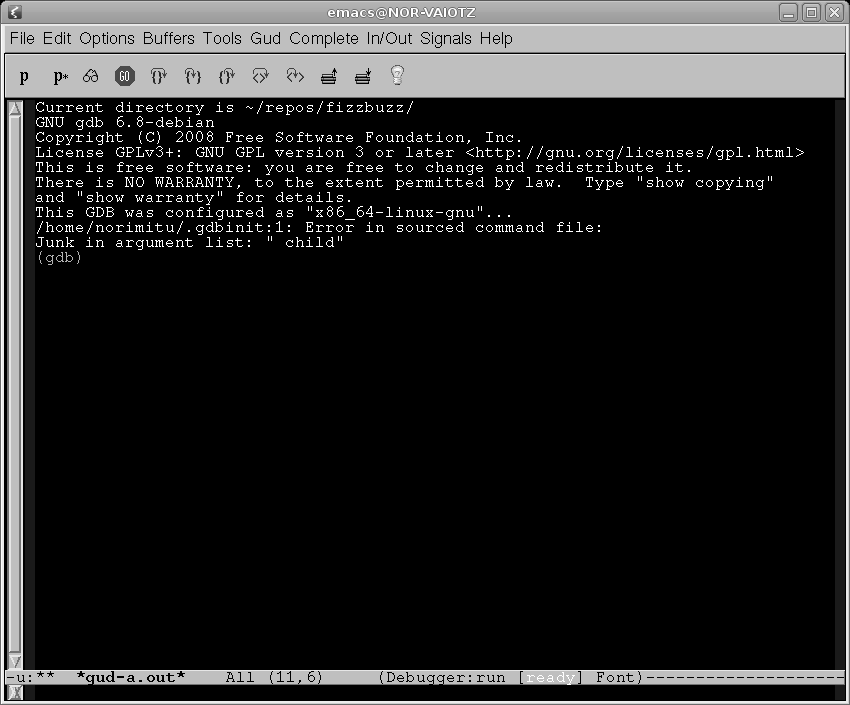
\includegraphics[scale=0.5]{image200910/gdb-emacs-gud1_mono.png}
\caption{Emacs GUDモードでgdbを起動した画面(1)}\label{figure-emacs-gud1}
\end{center}
\end{figure}

\begin{figure}[H]
\begin{center}
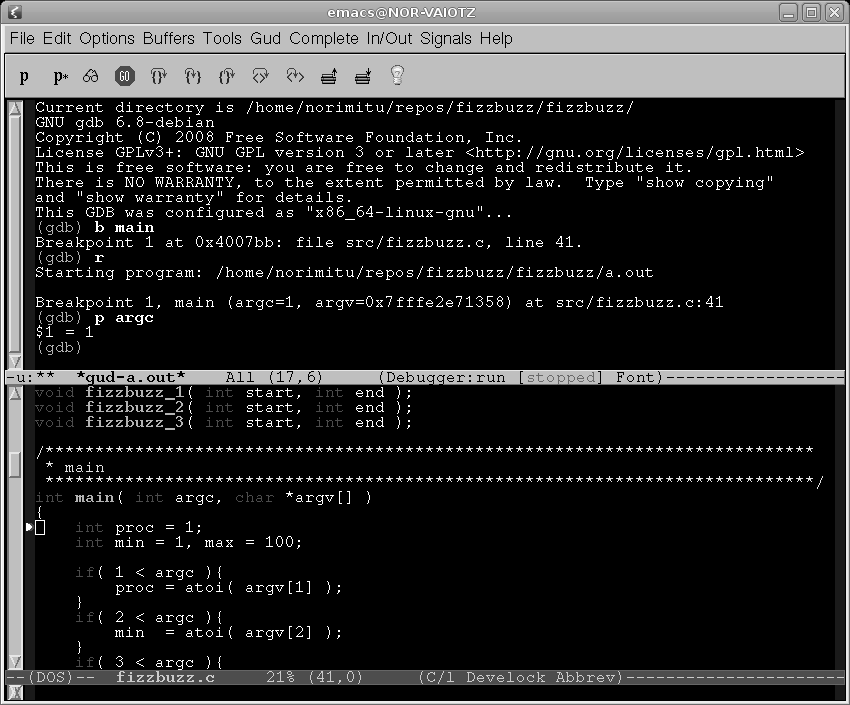
\includegraphics[scale=0.5]{image200910/gdb-emacs-gud2_mono.png}
\caption{Emacs GUDモードでデバッグ中の画面(2)}\label{figure-emacs-debugging1}
\end{center}
\end{figure}


また、Emacsの設定ファイル"〜/.emacs.el"に「(setq gdb-many-windows t)」を指定しておくと、すると図\ref{figure-emacs-gud2}、図\ref{figure-emacs-debugging2}のような画面でgdbが起動します。
この画面を表示するには「gud.el」というファイルが必要であり。lennyの場合はEmacsをインストールすると一緒にインストールされます。

\begin{figure}[H]
\begin{center}
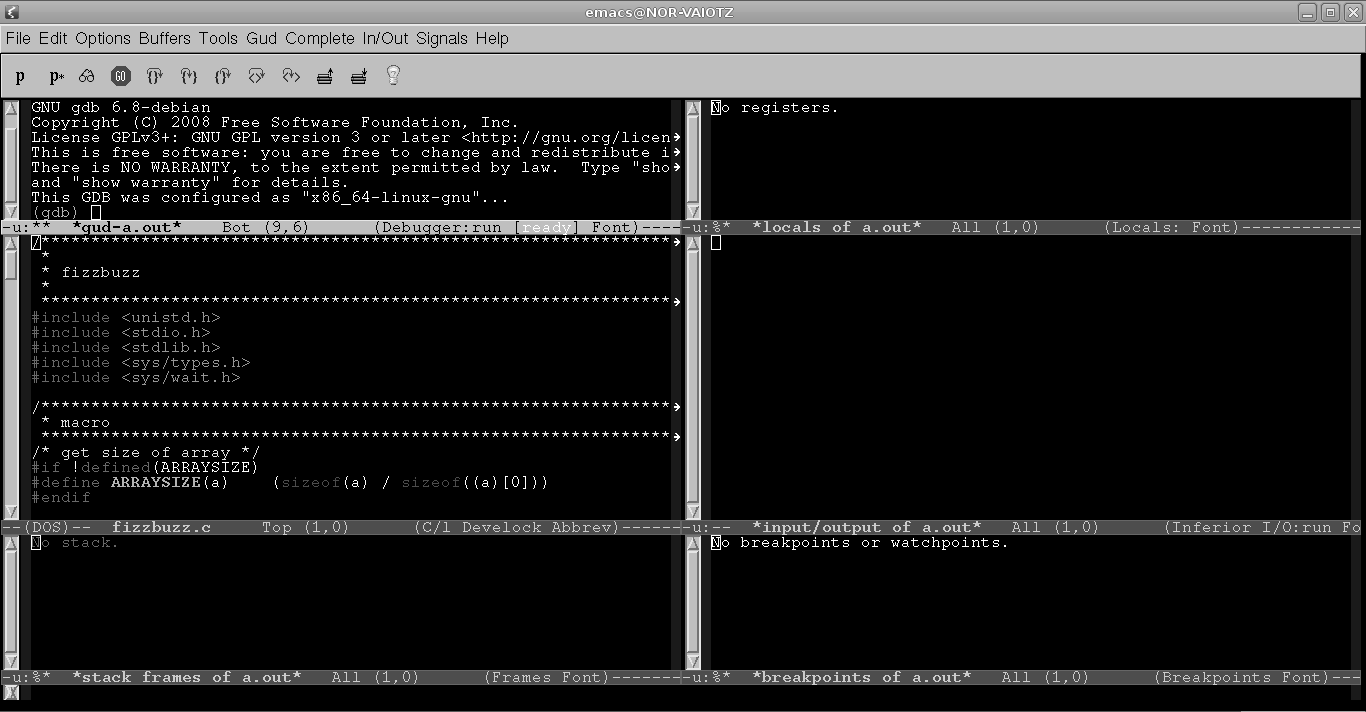
\includegraphics[scale=0.5]{image200910/gdb-emacs-gud3_mono.png}
\caption{Emacs GUDモードでgdbを起動した画面(3)}\label{figure-emacs-gud2}
\end{center}
\end{figure}

\begin{figure}[H]
\begin{center}
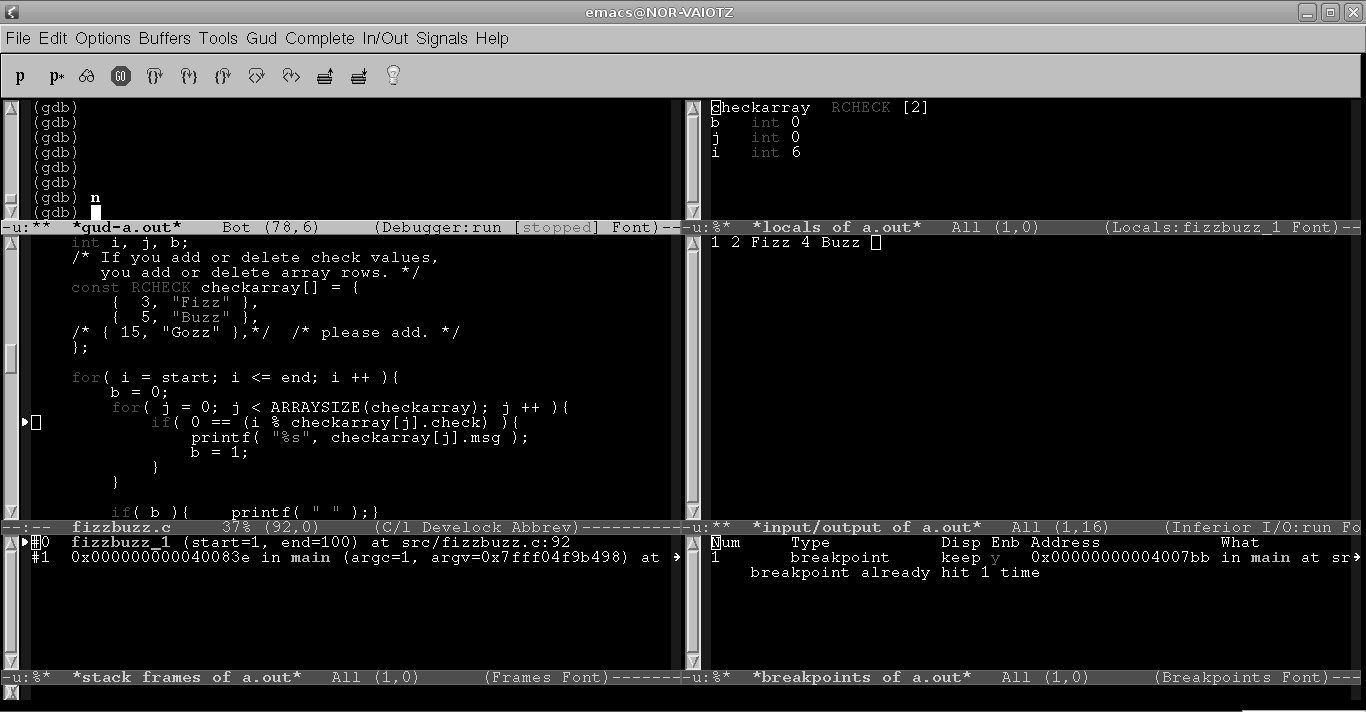
\includegraphics[scale=0.5]{image200910/gdb-emacs-gud4_mono.png}
\caption{Emacs GUDモードでデバッグ中の画面(4)}\label{figure-emacs-debugging2}
\end{center}
\end{figure}


\subsection{いろいろなプログラムのデバッグ方法}
私がプログラムをgdbを使ってデバッグするときの操作例を挙げてみます。

\subsubsection{単発実行系プログラムのデバッグ}
単発実行するプログラムの場合はデバッガでプログラムの起動を行い、その後にデバッグ作業を開始することになります。

\begin{enumerate}
\item gdbを起動します。
\item breakコマンドでブレークポイントを指定します。(実際には「b main」と入力してプログラムの最初で止めることも多いです。)
\item runコマンドでプログラムを開始します。
\item stepコマンド、nextコマンドでプログラムを追いかけます。
\item デバッグが完了したら、continueコマンドで残りのプログラムすべてを実行します。
\item quitコマンドでgdbを終了します。
\end{enumerate}

\subsubsection{デーモン系プログラムのデバッグ}
デーモンとして動作しているプログラムの場合は、動作中のプログラムをgdbで制御する必要があるためアタッチする必要があります。

\begin{enumerate}
\item デバッグするデーモンプログラムを実行します。
\item デバッグするデーモンプロセスのプロセスIDを調べます。
\item gdbを起動します。
\item プロセスIDを指定してattachコマンドを実行し、デバッグするデーモンプロセスにアタッチします。
\item breakコマンドでブレークポイントを指定します。(おそらく無限ループ処理のどこかで停止させることになると思います。)
\item ブレークポイントを設定したところでプログラムが一時停止しますので、stepコマンドやnextコマンドを実行してプログラムを追いかけます。
\item デバッグが終了したら、detachコマンドでプロセスからデタッチします。
\item quitコマンドでgdbを終了します。
\end{enumerate}

\subsubsection{forkするプログラムのデバッグ}
forkするプログラムの場合、fork()後に親プロセスと子プロセスのどちらを追いかけるのかを「set follow-fork-mode parent」などと設定しておく必要があります。

\begin{enumerate}
\item gdbを起動します。
\item 「set follow-fork-mode」を設定し、fork()後にデバッガを追うプロセスを親プロセスにするか、子プロセスにするか設定します。
\item breakコマンドでブレークポイントを指定します。
\item runコマンドでプログラムを開始します。
\item fork()した後は「set follow-fork-mode」で指定した親プロセスか子プロセスのいずれかを追従しますのでそのまま続けてデバッグします。
\item quitコマンドでプログラムを終了します。
\end{enumerate}

\subsection{まとめ}
今回はgdbの紹介とEmacs GUDモードにおいてプログラムをデバッグする一例を紹介しました。Emacs GUDモードを使ったデバッグ操作はX Window System上だけでなくコンソール環境でも同様の手順で実行できるため、telnet環境やssh環境でも同じスタイルでプログラムのデバッグ作業を行うことができます。

みなさんもDebianを使ってたくさんデバッグしてみましょう。

\subsection{参考資料}
\begin{itemize}
 \item man gdb(1)
\end{itemize}

\dancersection{GPG キーサインパーティの説明}{岩松 信洋}
\index{gpg}
\index{gpgきーさいん@gpgキーサイン}

\subsection{なぜキーサインするのか?}
\begin{itemize}
\item PGP/GnuPGは認証局がないので、自分が相手を信頼するしかありません。
\item 相手を信頼するには、キーサインパーティを行ってPGP/GnuPGの公開鍵をソーシャルな情報とともに交換し、信頼の輪(web of
 trust)を広げる必要があります。
\end{itemize}

\subsection{使いどころ:フリーソフトウェア開発者の場合}
\begin{itemize}
\item アカウント作成時のチェックに利用する場合があります。(インターネット上での存在を
      示す。)
\item ソフトウェアのリリース時に利用する場合があります。
\item Debian ではパッケージへの署名、投票などに使います。
\end{itemize}

\subsection{使いどころ:ユーザの場合は?}
\begin{itemize}
\item メールへの署名/暗号化に利用する場合があります。
\item Debian Project 公式開発者になるための通過儀礼の一つです。
\end{itemize}
身近なところでは、改竄のチェックに使います。
Debian の場合は secure-apt で使われています。

Debian アーカイブの鍵が更新されていなかったり、アップデートされていない
と以下のようになります。
\begin{commandline}
# apt-get update
.....
W: GPG error: http://cdn.debian.or.jp testing Release: The following
 signatures couldn't be verified because the public key is not
 available: NO_PUBKEY 9AA38DCD55BE302B
\end{commandline}

このような状態になった場合には、GPGの鍵サーバからsecure-apt用の最新の鍵を取得し、更新
します。最新の鍵については\url{http://ftp-master.debian.org/keys.html}を
参照してください。以下に更新の例を示します。

\begin{commandline}
# gpg --keyserver wwwkeys.eu.pgp.net --recv-keys 9AA38DCD55BE302B
# gpg --armor --export 9AA38DCD55BE302B | apt-key add -
# apt-get update
.....
Fetched 2B in 1s (1B/s)
Reading package lists... Done
\end{commandline}
何も考えずにやると上記のようになりますが、これではいけません。
鍵を更新する前にちゃんと鍵と信頼度をチェックしましょう。{\bf エラーがでなくなった!これで大丈夫!(って書いてあるWebサイト多
 いよね。)と思ってはだめです。}
%詳しい更新方法については武藤さんのblog\{http://kmuto.jp/d/index.cgi/debian/apt-secure.htm}
%を参考にするとよいでしょう。
もちろん、鍵のチェックにはWeb Of Trustに入らないとできません。

\subsection{チェックする簡単な方法}
では、鍵をチェックするにはどうしたらいいのでしょうか。
例えば、9AA38DCD55BE302B の鍵に署名している人は以下のとおりです。

\begin{commandline}
pub  4096R/55BE302B 2009-01-27            
uid Debian Archive Automatic Signing Key (5.0/lenny) <ftpmaster@debian.org>
sig  sig3  55BE302B 2009-01-27 _____ 2012-12-31 [selfsig]
sig  sig   7E7B8AC9 2009-01-27 _____ __________ Joerg Jaspert <joerg@debian.org>
sig  sig   D0EC0723 2009-01-27 _____ __________ Mark Hymers <mhy@debian.org>
sig  sig   BE9BF8DA 2009-01-27 _____ __________ Mike O'Connor (stew) <stew@vireo.org>
sig  sig   30B94B5C 2009-05-24 _____ __________ XXXXXXXXX (imacat) <imacat@mail.imacat.idv.tw>
\end{commandline}
\footnote{imacatの名前は文字化けのためXXXXXXXX にしてあります。}

まず、公開鍵を取得し鍵のチェックを行います。
\begin{commandline}
$ gpg --keyserver pgp.mit.edu --recv-keys 55BE302B
$ gpg --list-sig 55BE302B
pub   4096R/55BE302B 2009-01-27 [満了: 2012-12-31]
uid                  Debian Archive Automatic Signing Key (5.0/lenny)
<ftpmaster@debian.org>
sig          7E7B8AC9 2009-01-27  [ユーザーIDが見つかりません]
sig          D0EC0723 2009-01-27  [ユーザーIDが見つかりません]
sig          BE9BF8DA 2009-01-27  [ユーザーIDが見つかりません]
sig          30B94B5C 2009-05-24  [ユーザーIDが見つかりません]
sig 3        55BE302B 2009-01-27  Debian Archive Automatic Signing Key (5.0/lenny) <ftpmaster@debian.org>
\end{commandline}
この結果から、この鍵にサインしている人とは、直接GPGサインしていないこと
がわかります。

\subsection{trust path finder}
しかしWeb of Trust なので、信頼のパスが使えます。\\
trust path finder\footnote{\url{http://pgp.cs.uu.nl/mk_path.cgi}}を使う
とGPGの信頼のパスが分かります(図\ref{fig:trust-path-example})。\\

\begin{figure}[h]
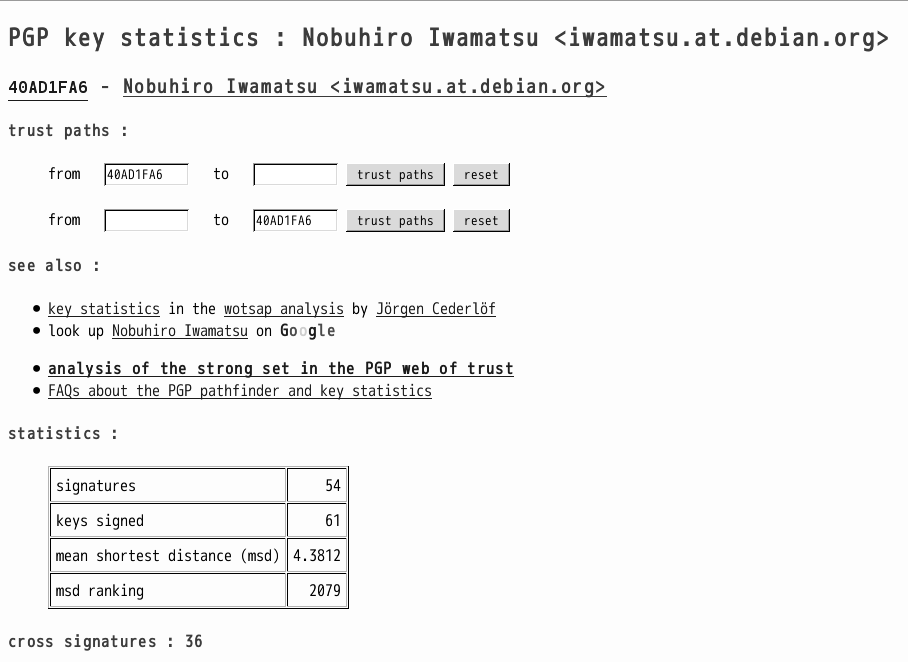
\includegraphics[width=0.8\hsize]{image200909/trust-path_mono.png}
\caption{GPGの信頼のパス}
\label{fig:trust-path-example}
\end{figure}

\subsection{Joergと岩松の信頼のパス(trust path)}

Debian FTP masterであるJoergと岩松の信頼のパスを調べると図
\ref{fig:trust-path-joerg-iwamatsu}のようになります。

\begin{figure}[h]
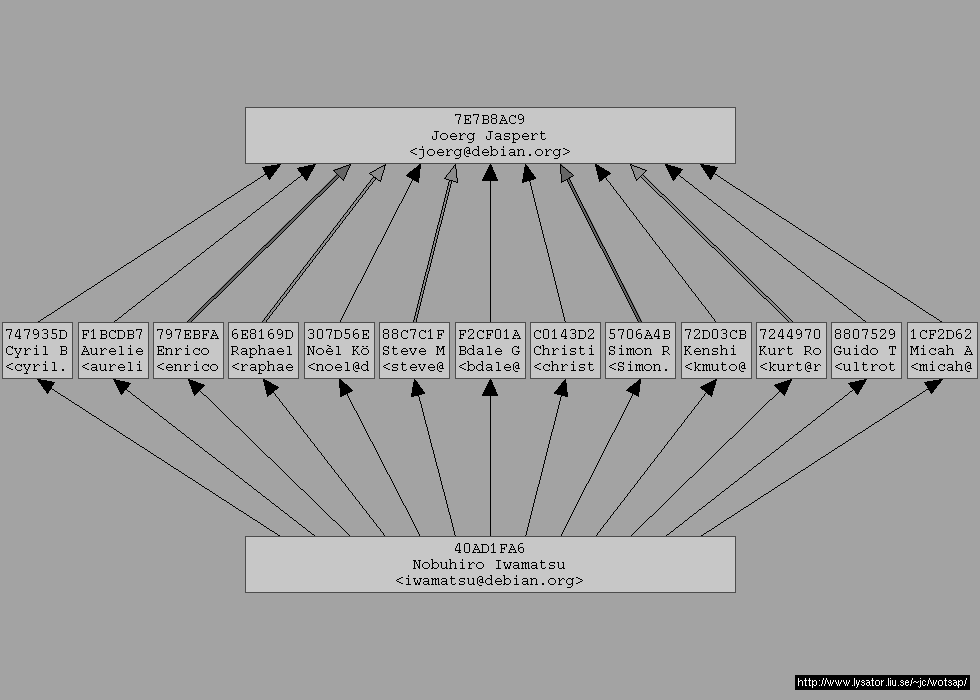
\includegraphics[width=0.8\hsize]{image200909/0x40AD1FA6-0x7E7B8AC9_mono.png}
\caption{GPGの信頼のパス}
\label{fig:trust-path-joerg-iwamatsu}
\end{figure}

他の人を介して、Web of Trust がつながっていることが分かります。
知り合いの知り合いがサインしているようです。ちょっとは信用できるかな?

\subsection{キーサインの流れ}

さて、実際のキーサインの流れを見てみましょう。
簡単な流れは図\ref{fig:gpg-key-sigining}のようになります。

\begin{figure}[h]
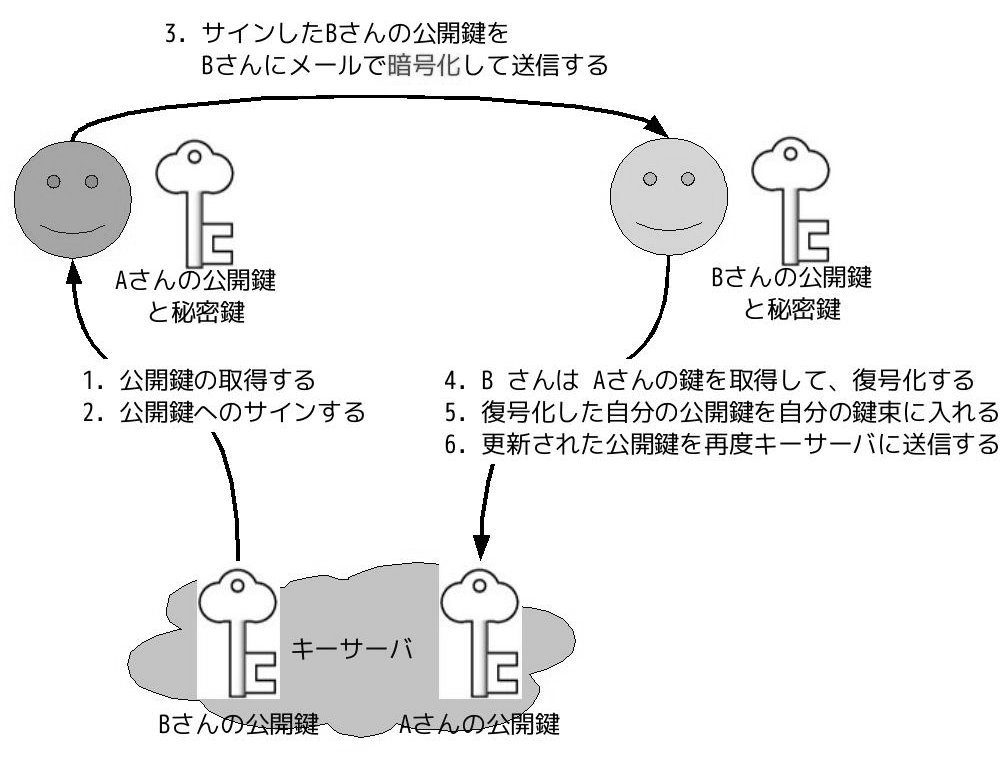
\includegraphics[width=0.8\hsize]{image200909/gpg-key_mono.jpg}
\caption{キーサインの流れ}
\label{fig:gpg-key-sigining}
\end{figure}

\subsection{gpg コマンドでやった場合}

キーサインをコマンドで行うと以下のようになります。
\begin{commandline}
$ gpg --keyserver pgp.mit.edu --recv-key 40AD1FA6
$ gpg --fingerprint 40AD1FA6
$ gpg --edit-key 40AD1FA6
$ gpg --sign-key 40AD1FA6
$ gpg --check-sig 40AD1FA6                   
$ gpg --export -a 40AD1FA6 > iwamatsu.gpgkey   
$ iwamatsu.gpgkey を 相手にメールに 署名+暗号化して送信
\end{commandline}

数人ならいいけど、キーサインパーティでは100人ぐらい集まることもあります。
100人分もコマンドであるとなると大変です。

\subsection{そこでcaffの登場}

上記のような場合、caff を使って行うと作業が大変楽になります。
caff は signing-party パッケージで提供されています。
インストール・初期化の手順を以下に示します。

インストールはいつものapt-getで行えます。
\begin{commandline}
$ sudo apt-get install signing-party
\end{commandline}

次にcaff を使うための初期化を行います。
caff を一回実行すると、ホームディレクトリ下に初期ファイル{\bf .caffrc}を
作成してくれます。
\begin{commandline} 
$ caff
.......
#
#Regards,
#{$owner}
#EOM

Please edit /home/hoge/.caffrc and run caff again.
\end{commandline}

\subsection{caffの設定}
次に \~{}/.caffrc にある 設定ファイルを修正します。
\begin{commandline}
$ cat ~/.caffrc

$CONFIG{'owner'} = 'Nobuhiro Iwamatsu';
$CONFIG{'email'} = 'iwamatsu@debian.org';

$CONFIG{'keyid'} = [ qw{4121C7433170EBE9 32247FBB40AD1FA6} ]

# Additionally encrypt messages for these keyids
$CONFIG{'also-encrypt-to'} = [ qw{4121C7433170EBE9 32247FBB40AD1FA6} ]

# Mail template to use for the encrypted part
$CONFIG{'mail-template'} = << 'EOM'\maketitle#Hi,

please find attached the user id{(scalar @uids >= 2 ? 's' : '')}
{foreach $uid (@uids) {
    $OUT .= ``\t''.$uid.''\n'';
};}of your key {$key} signed by me.
......

\end{commandline}


\subsection{caffの設定}          

caff のデフォルトの設定では、cert-digest-algo が SHA1 になっているので、
 \footnote{http://bugs.debian.org/cgi-bin/bugreport.cgi?bug=527944} SHA512に
 設定します。
\begin{commandline}
$ mkdir -p ~/.caff/gnupghome
$ chmod 700 ~/.caff/gnupghome
$ cat >> ~/.caff/gnupghome/gpg.conf
cert-digest-algo SHA512
personal-digest-preferences SHA512
EOF
\end{commandline}

また、サインした鍵をメールで送信するので、ローカル(作業するマシン)のSMTPも設定しておく必
要があります。

\subsection{caffを使った署名}

以下のように実行すると、署名するID をキーサーバから取得し、指定した自分
のIDで署名してくれます。
そして、署名した鍵を暗号化して送信してくれます。

\begin{commandline}
$ caff -u 自分のID 署名するID .......
\end{commandline}

\subsection{署名完了後}
署名後のデータは \~{}/.gnupg/pubring.gpg ではなく、{\bf \~{}/.caff/gnupghome/pubring.gpg} に格納
 されています。この鍵束を \~{}/gnupg/pubring.gpg に 取り込む必要がありま
 す。以下の方法で取り込む事が可能です。
\begin{commandline}
$ gpg --import ~/.caff/gnupghome/pubring.gpg
\end{commandline}

取り込んだら、自分の鍵をキーサーバに送信します。
\begin{commandline}
$ gpg --keyserver pgp.nic.ad.jp --send-keys 自分のID
$ gpg --keyserver pgp.mit.edu --send-keys 自分のID
\end{commandline}


\subsection{最後に}
相手に鍵を送るまでがキーサインパーティです。
ちゃんと相手に署名した鍵を送りましょう。

\dancersection{DDTSS を使ってみよう}{倉敷 悟}
\index{DDTSS}
\index{DDTP}
\index{Debian Description Translation Project}

\subsection{そもそも DDTSS って何?}

シンプルに言うと、「パッケージ説明文」を翻訳するための Web インターフェイスのことです。

解説資料としては、第53回東京エリアDebian勉強会の資料
(\url{http://tokyodebian.alioth.debian.org/2009-06.html})でまとめられています。
今回は、この資料を参照しながら、ハンズオンとして実際に DDTSS を使った翻訳作業をやっていきます。

\subsection{事前課題の確認}

今回は、準備として事前課題の形をとってみましたが、いかがでしたでしょうか。

今後のセッションでも、適宜事前課題をからめていきたいと思っていますので、気づいたことがあれば教えてください。

\subsubsection{DDTSS アカウントの作成}

DDTSS はウェブサービスで、ユーザのアカウントを独自に保持しています。
作業内容や実績はアカウントとひもづけて保管されるので、最初に作っておきましょう。\footnote{DDTSS create login \url{https://ddtp.debian.net/ddtss/index.cgi/createlogin}}
ユーザ ID として利用される、メールアドレスが必要になります。

では作成したアカウントで、DDTSS にログインしてみてください。作成がまだの人はここで作ってしまいましょう。

\subsubsection{気になるパッケージを探す}

DDTSS の翻訳で扱う「パッケージの説明文」は、個別にはあまり量もないですし、翻訳作業をするにあたって、とっかかりの敷居は低い方だと思います。

とはいえ、見たことも聞いたこともないパッケージの説明というのもやっぱり辛いものがありますので、まずは関心があるとか、使っているとか、見たことある、といったものから手をつけてみるといいでしょう。

\subsection{レビューをしてみる}

DDTSS では、誰かが訳した一つの説明文は、オフィシャルの配布データにとりこまれるまでに、3 人からレビューを受けて「修正なしで OK」とされる必要があります。

レビュー 3 人というのは、実は結構高いハードルで、ついついレビュー待ちのものがたまってしまいがちです。

そういうわけで、いきなり翻訳するというのはしんどいなぁ、という方も、ひとまずレビューにチャレンジしてみましょう。
すでに翻訳された文章を確認するだけなので、敷居は低いと思います。

この文章を書いている時点では、レビュー待ちの数がずいぶん少ないので、選ぶのに困ってしまうかも知れませんが……。

\subsubsection{レビュー待ち一覧の見方}

DDTSS のログイン画面を、下の方にスクロールしてみてください。
「Pendingreview」と書かれたセクションがあるはずです。
下に並んでいるパッケージが、レビューを待っているもので、「Pending review」の横にある数字はその合計数になります。各パッケージ名の横を見ると、レビューの状況がわかります。

「needs initial review」は、翻訳された後まだ一回もレビューされていないということです。

「needs review had x」は、レビュー途上にあるもので、x がレビューされた回数を示しています。

\subsubsection{レビュー画面}

ではパッケージを選んでみましょう。レビュー画面に切り替わります。
いくつかのメタ情報と合わせて、パッケージの説明文が、原文と対比される形で表示されているはずです。

まず、訳文を読んでみてください。意味は通りますか?  誤字はありませんか?
おかしいな、と思ったところは、原文と見比べてみてください。

レビューしてみて、特に訂正が必要ない状態であれば、「Accept as is」ボタンを押します。これで、レビューカウントが 1 つ増えることになります。

これはどう見てもおかしいな、というところがあれば、フォームの上で編集して、「Accept with changes」ボタンを押します。
訳文は変更されて、レビューは振り出しに戻ることになります。

ちょっと違う気がするんだけど、いまいち自信がない……という場合は、コメント欄 (comment field) がありますので、そこに書いて、「Change comment only」ボタンを押します。この場合、レビューとしては何も変更されず、コメントだけ追記されることになります。

開いてみたけど、やっぱりレビューをやめる、という場合は、何もボタンを押さずに戻ってください。

\subsubsection{実際にレビューしてみる}

少しまとまった時間をとりますので、レビューにチャレンジしてみてください。
わからないことがあれば、適宜呼んでください。

\subsection{最初の翻訳文作成}

いくつかレビューをしてみて DDTSS にも慣れてきたら、翻訳にも手を出してみてください。
翻訳されていないパッケージ説明文は、「Pending Translation」の一覧にあります。気になるものを選んでみましょう。

画面の構成は、レビューとほとんど同じですが、翻訳文は、あったりなかったりします。
翻訳文がある場合でも、原文が更新されていたり、似ている別のパッケージからひっぱられたりしているので、何らかの修正は必要になるはずです。

実際の翻訳画面にも赤字で表示されますが、やっぱり翻訳をやめる、という場合には「Abandon」というボタンを押すことになっているので注意してください。

ここは、時間が許せば実際にやってみようと思います。

% ===============================================================
\dancersection{DDTP 翻訳作業での TIPS}{あけど}
\index{DDTSS}
\index{DDTP}
\index{Debian Description Translation Project}
% ===============================================================

\subsection{はじめに}


Debian Package をインストールする際に参考する情報、{\bf Description} 昔は
すべて英語でしたが、最近はすこしづつ日本語になってきているのはご存知でし
たか?
Debian Description Translation Project は Debian Package の Description
文(パッケージの内容を説明する文章)を日本語にするためのプロジェクトです。
\footnote{DDTPサイト: \url{http://ddtp.debian.net/}}

日本語の翻訳の進捗は図 \ref{fig:transstatja} の状況です。

\begin{figure}[h]
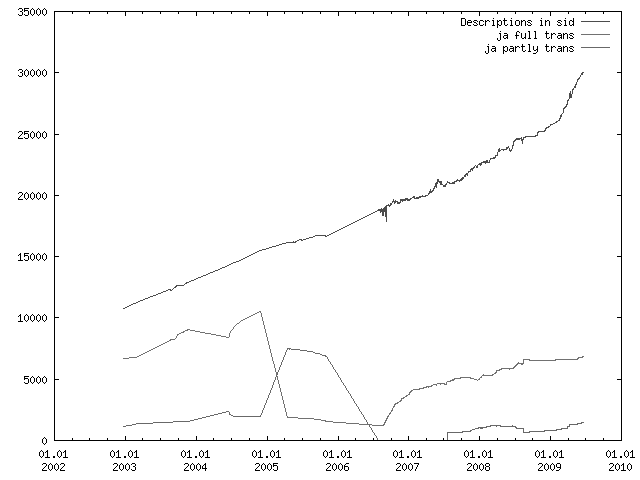
\includegraphics[width=0.5\hsize]{image200906/stat-trans-sid-ja_mono.png}
\caption{日本語の状況}
\label{fig:transstatja}
\end{figure}

前回、5月の東京エリアDebian勉強会でトピックに挙っていました DDTSS につい
て、作業上の留意点などをまとめてみました。DDTSS については運用ルールなど
で明確になっていない部分もありますので、その議論を深める材料になればと思います。
このセクションはこれから翻訳を始めてみようという方へのガイドとしても考慮した
つもりです。
なお、このセクションにおいての幾つかの見解は筆者の個人的見解が多分に含まれて
いますので、その点ご留意頂ければと存じます。

\url{http://tokyodebian.alioth.debian.org/pdf/debianmeetingresume200905.pdf}
 p.31「8 DDTSS 活用」

\subsection{ガイド等の文書の把握}
5月の資料にまとまっていますが、その後に作成されたページをご案内します。

\begin{itemize}
 \item DDTSS\_ja/Faq - Debian Wiki
% ja/DDTSS_ja/Faq - Debian Wiki
       \url{http://wiki.debian.org/ja/DDTSS_ja/Faq}
\end{itemize}

以下は5月の再掲です。
\begin{itemize}
 \item Debian パッケージの説明文を日本語で読みたい! 〜DDTP へのお誘い〜 
       \url{http://www.debian.or.jp/community/translate/description-ja.html}
 \item 武藤健志さんのblogの『Debianドキュメント翻訳手続き』:
       \url{http://kmuto.jp/d/index.cgi/debian/debian-doc-procedure.htm}
 \item 小林儀匡さんのDebian勉強会2006年9月資料「翻訳への誘い」:
       \url{http://tokyodebian.alioth.debian.org/pdf/debianmeetingresume200609.pdf}
 \item debian-doc メーリングリスト:
       主要な議論が行われています。質問なども、こちらで。
\end{itemize}

\subsection{翻訳(辞書)サイトの利用}
翻訳するのに十分な知識があればそもそも辞書は必要無いのかも知れません。
印刷された辞書を使うのはインターネット接続がない環境では有効ですが、
コンピュータを使う現代的な環境であればインターネット接続はほぼ不可欠でしょうから、
オンラインの翻訳サイトを利用しない手はありません。
以下にお勧めのサイトをご紹介します。

\begin{itemize}
 \item{英単語辞書
  \begin{itemize}
   \item{英辞郎 on the web スペースアルク \url{http://www.alc.co.jp/}
収録単語の量、質、訳がそれぞれ秀逸です。
スラング等の現代語から専門用語まで幅広く、また対象の英単語が含まれる例文が実例に基づいていて実用的な訳を得られます。
(※このサイトを利用しているだけで、中学、高校で受けた英語が英文学を主眼に置いたものだと実感しました。)}
  \end{itemize}
 }
 \item{文章翻訳
  \begin{itemize}
   \item{Yahoo!翻訳 \url{http://honyaku.yahoo.co.jp/}
   文単位での訳と原文の対応が付くので、長い文章や複雑な文章の翻訳に向いています。}

   \item{英語翻訳 - エキサイト 翻訳
     \url{http://www.excite.co.jp/world/}
   自然な表現の日本語訳を得られます。カタカナ語の訳語をかなり上手く当てはめてくれたりします。}

   \item{Cross Translation::色々な翻訳サイト・翻訳サービスの一括、横断翻訳
     \url{http://sukimania.ddo.jp/trans/trans_e.php}
   上記のYahoo!翻訳、エキサイト 翻訳などの翻訳サービスにて一括で翻訳するサービスです。
   翻訳に迷った時の参考になるでしょう。但し、全てのサイトでの結果を得るには多少時間がかかります。}
  \end{itemize}
  他にも辞書・翻訳サイトは多数ありますので、各自で探してみて下さい。
 }
\end{itemize}


\subsection{Google で 「Debian」+「対象のパッケージ名」を検索}
Debian パッケージの過去バージョンで既に翻訳されている事がありますので
それを参考にすることもできます。

(注: DDTSSに訳が取り込まれていない場合があるのです。)


\subsection{分かりやすい文章にするための幾つかの手法}
\begin{itemize}
\item {直訳の表現が日本語的に分かり難い場合

 意訳した方が分かりやすいならその方が望ましいです。}

\item{ドイツ系の人が書いた英語で、関係代名詞が多用されていて直訳では日本語とし
     て分かり難い文章になることがよくあります。

 そういった場合には、文を分かりやすいサイズに区切りましょう。}

\item{専門用語と思われる訳語が直訳では意味が分かりない事があります。

 専門用語はその分野での良く使われる訳語の表現を調べるようにしましょう。

      (注:下記に注意点をまとめました)}
\end{itemize}

\subsection{DDTSS 限定TIPS}
\begin{itemize}
 \item{コメント欄の活用

  そのパッケージの翻訳に関しての注意事項などをレビューする人に向けて書いておくとレビューの際の参考になります。
   専門用語や意訳など、普通とは違う翻訳をした場合などにその理由などの
   根拠を書いておくと次の段階のレビュー作業をする人に理解してもらいやすくなります。
 }

 \item  Accept with changes がクリックできない場合

 翻訳文だけを更新した時に Accept with changes がグレーアウトしたままでクリックできないときがあります。
タイトル部を変更することで対応できます。以下はその手順です。
 \begin{enumerate}
  \item タイトルに空白等を追加する。
  \item Tab キーで次フォームにカーソルを移動すると、
	タイトルが更新されたとみなされ Accept with changes がクリック出来るようになります。
  \item タイトルに追加した空白等の文字を削除し、元に戻します。
  \item Accept with changes をクリックします。
 \end{enumerate}

\end{itemize}


\subsection{専門用語の扱い}
\begin{itemize}
 \item{専門用語の見分け方

決め手はありません。
パッケージの説明に記述された関連分野から推測するか、その分野について(必要に応じて)調べる事を念頭に置いて作業するのが良いでしょう。}

 \item{パッケージ説明で良く見かける専門分野とその専門用語及び良く使われ
      ている訳語} \footnote{ この段落付近は筆者の経験に大きく依存しています。}
 \begin{itemize}

  \item 生物学、バイオインフォマティックス (biology, bioinfomatics)

        DNA 解析に関するパッケージが多数あります。

	annealing: アニーリング、(遺伝アルゴリズムの焼きなまし法
	(Simulated Annealing)、機械加工の熱処理とは別のもの)

	align, alignment: アライン、アライメント、整列

	multiple alignment: マルチプルアライメント

	multiple sequence alignment: マルチプルシークエンスアライメント、(複合配列整列)

	polymerase chain reaction: ポリメラーゼ連鎖反応、略語 PCR、ポリメレースチェーンリアクション

	sequence: シークエンス、(遺伝子などの)配列


  \item アマチュア無線 (hamradio)
	band: 周波数帯、バンド

	CW: 電信

	modem: モデム

	Sporadic E layer: スポラディックE層 (sporadicを突発的と訳さないのが一般的です。)

	N meter band: Nメーターバンド (波長を周波数帯の別名として呼ぶのはアマチュア無線では一般的です。)


  \item その他、複数の分野にまたがる用語

	Markov chain: マルコフ連鎖 統計学、数学、物理学、統計力学、情報科学

  \end{itemize}

\end{itemize}


\subsection{専門用語の訳についてのルール}
どう扱うかのルールは未だ決まっていません。

 現状の対応

各々の分野のサイトでの表記を参考にしています。

良く使われる表記が複数ある場合はケースバイケースで妥当と思われるものを採用しています。

例) muliple sequence alignment の訳語
\begin{enumerate}
 \item 多重配列整列
 \item 多重配列アライメント
 \item マルチプルシークエンスアライメント
\end{enumerate}


この様な専門用語について今まで耳にした意見を挙げてみます。
\begin{enumerate}

 \item 日本語より英語での表現が一般的であれば訳さない方が利用者にとって
       便利なので、訳さないかせいぜいカタカナにして持ってくるのが良い。
例)
CPU,メモリ、DHCP,etc

 \item 日本語の訳が複数あり、利用状況がまちまちであるなら上記の案を勘案
       してパッケージ検索時の利便性を重視して、日本語の表記に()括弧内に
       原文の語を示すのはどうか?

例) muliple sequence alignment

 1. 多重配列整列 (muliple sequence alignment)

 2. 多重配列アライメント (muliple sequence alignment)

 3. マルチプルシークエンスアライメント (muliple sequence alignment)

日本語の表記にばらつきがありますが、パッケージ検索で意図した内容は実現で
きそうです。ただし、この様な語句が多いと見やすさを損なうかもしれません。

 \item その他、ご意見募集中
\end{enumerate}

\subsection{最後に}
記述にあたって、様々な方々との(会話なども含む)やり取りを参考にしました。
翻訳サイトの案内については吉田@板橋さんの小江戸らぐでの発表を参考にしました。
DDTSSでの作業についての助言や、このセクションの構成については、やまだたくまさん
からのアドバイスを参考にしました。
また、他の皆さんからのご意見が大変参考になりました。そういったものもできるだけ盛り込んだつもりです。
DDTSSにより翻訳作業のしきいは大きく下がったと思います。
様々な人が少しでも多くDDTSSで翻訳作業に参加できるようになれば、作業の量
だけでなく質も向上させることができると期待できます。

\subsection{追加:第53回東京エリアDebian勉強会で出された意見}
\begin{itemize}
 \item 日本語としての自然さなど、翻訳の質が一定しないのはどうかと思う。

 $\rightarrow$何か基準があれば良い?

 $\rightarrow$でも、基準を作るのは難しいし、それより沢山の人が色々な観点からレビューする方が有効ではないか? 

 \item 翻訳のコツとして心がけていること

\begin{itemize}
 \item   直訳より、日本語として分かり易い文章になるようにする。

 \item  長文は短文に分割する。

 \item  形容詞が連続する部分は(強調の意味が大きいので)意図的に訳さない。 
\end{itemize}

 \item DDTSS 利用上の注意点

  ログインしなくても翻訳できてしまうので必ずログインするようにしましょう。

 \item 専門用語について

  下手に日本語に訳されていると検索で見つからないので、敢えて訳さずに原文のままの方がいい

  $\rightarrow$ LANG=C aptitude search 〜 とすると英語での検索になるが、それではどうか? 

  専門用語の訳語が複数あって適用される状況がまちまちな場合があるが、どう
       するのが良いか?

       $\rightarrow$ガイドラインを設定するのはどうか?

       $\rightarrow$ガイドラインを用意するのは難しいし、それより適用事例をまとめたもの
       を用意した方が使いやすい


 \item 翻訳が未経験または自信の無い人はレビューから始めたらどうか

 \item OmegaT のような翻訳ツールを活用して翻訳辞書(翻訳事例)を共有できると、翻訳の質が安定するのでは?

  $\rightarrow$ OmegaT についてはもっと情報を集める必要がある

\end{itemize}

% ===============================================================
\dancersection{DDTSS の利用方法の紹介}{やまだたくま}
\index{DDTSS}
\index{DDTP}
\index{Debian Description Translation Project}
% ===============================================================

\subsection{はじめに}
Debian パッケージの説明文を翻訳するプロジェクト DDTP にある Web インタ
フェース DDTSS の使い方を簡単にご紹介します。

\subsection{アカウント作成とログイン}

\url{http://ddtp.debian.net/ddtss/index.cgi/ja} を開いて、一番下にある Create
Login をクリックします。

  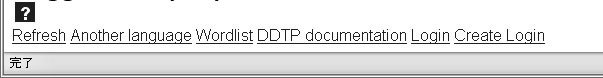
\includegraphics[scale=0.7]{image200906/ddtss129_mono.jpg}

E メールアドレス (Email Address)とログイン名(Alias)、本名(Real Name)、パスワードを 2
回入力(Password, Retype Password)して Submit ボタンを押して送信すると、
アカウント作成は完了です。Alias は各種ログの表示で使われます、英文字のわ
かりやすい表記にしましょう。

  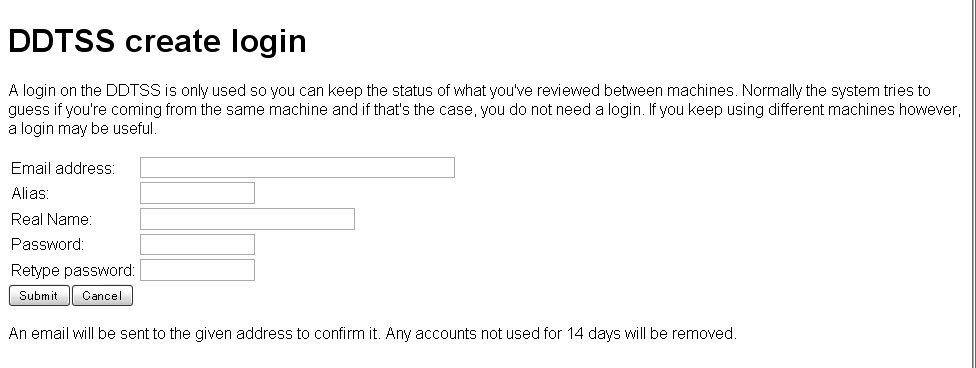
\includegraphics[scale=0.7]{image200906/ddtss141_mono.jpg}

アカウントを作成したらログインします。作業画面の右上にアカウントの情報が表示されます。

  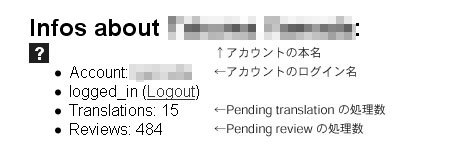
\includegraphics[scale=0.7]{image200906/ddtss130_mono.jpg}

\subsection{DDTSS で行ってほしい作業 - レビュー}

現在 DDTSS でもっとも必要な作業は「レビュー」です。レビューの対象は、次の場所に表示されています。

\begin{commandline}
Pending review (98)

   1. bristol (needs initial review)
   2. pngquant (needs initial review)
   3. adesklets (needs initial review)
   4. inventor-demo (needs initial review)
   5. emboss (needs review, had 1)
\end{commandline}

パッケージ名をクリックすると内容が表示されます。その内容を見て、簡単そうならレビューをします。
難しいと思ったら、次のパッケージへ飛ばしてかまいません。

  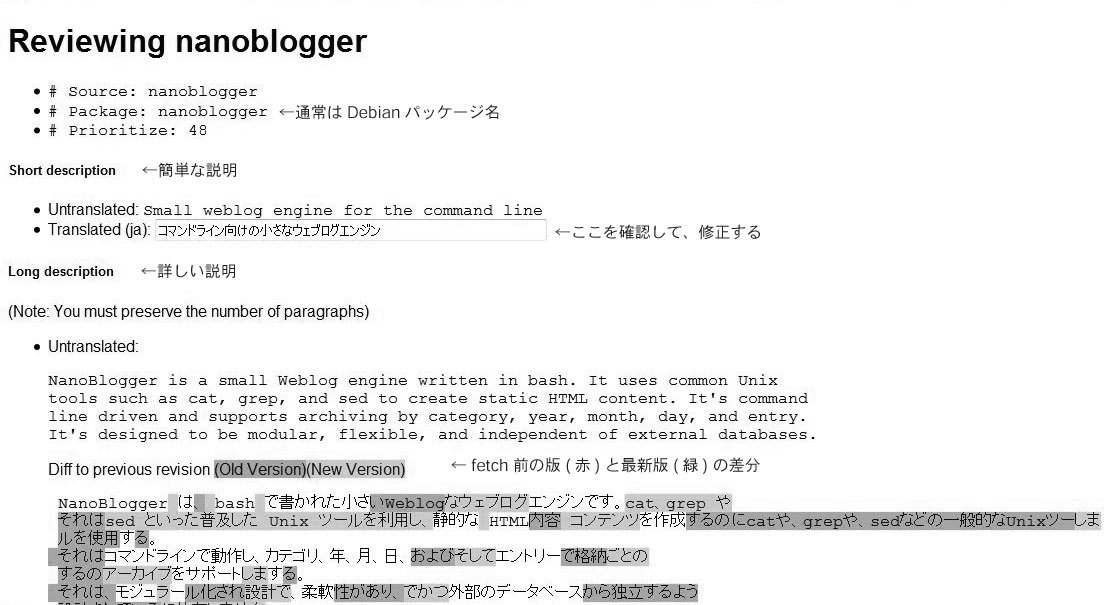
\includegraphics[width=170mm]{image200906/nanoblogger101_mono.jpg}

  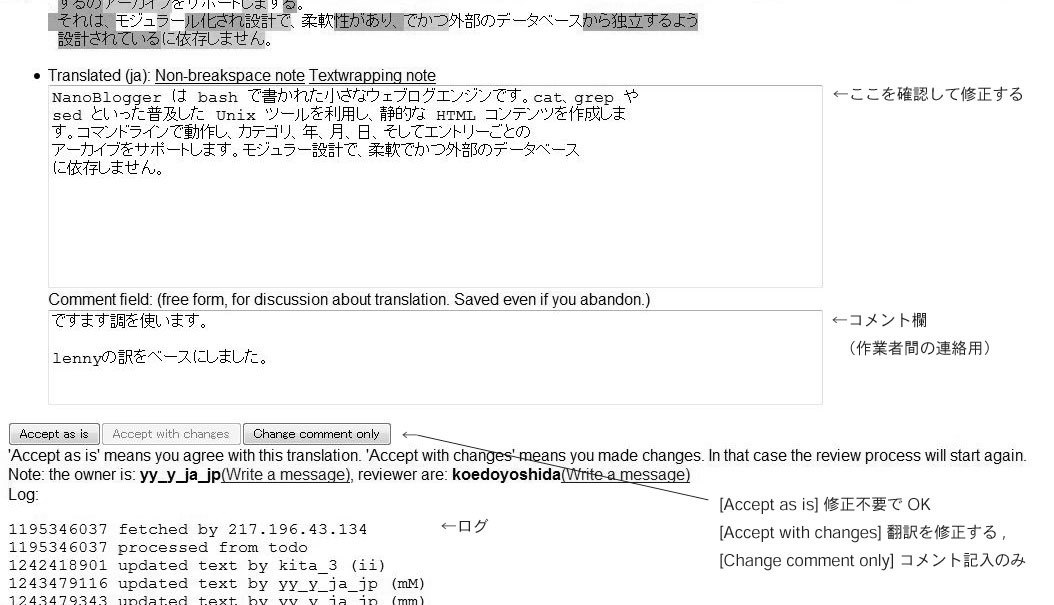
\includegraphics[width=170mm]{image200906/nanoblogger102_mono.jpg}

  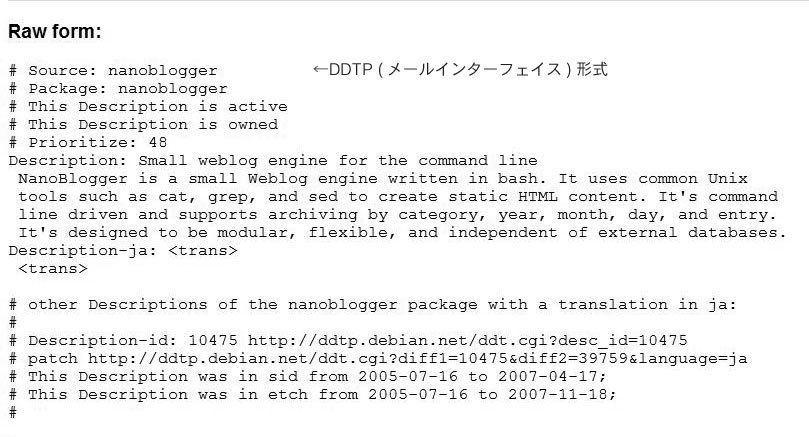
\includegraphics[width=130mm]{image200906/nanoblogger104_mono.jpg}

\subsection{レビューする}

翻訳内容に問題ないと判断できた場合は、[Accept as is] ボタンをクリックしてください。

  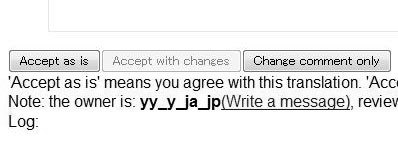
\includegraphics[scale=0.7]{image200906/nanoblogger112_mono.jpg}

レビューをすると、表示される場所が変わります。さらにレビューが必要な場合
は、次のようになります。

  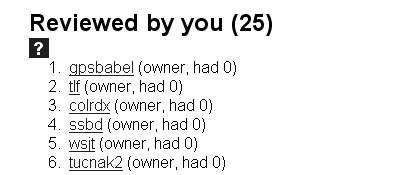
\includegraphics[scale=0.7]{image200906/ddtss131_mono.jpg}

連続して 3 人がレビューをすると、翻訳作業が完了します.完了後は次のように
なります。

  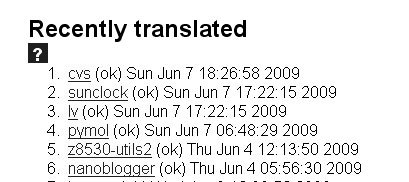
\includegraphics[scale=0.7]{image200906/ddtss132_mono.jpg}

途中で誰かが翻訳を修正したら、再び 3 人のレビューが必要になります。

\subsection{レビューを修正する}

翻訳内容にすぐ修正が必要なら、テキストを変更してから [Accept with
changes] ボタンをクリックしてください。なるべくコメント欄 (Comment
field) に変更内容を記入してください。

  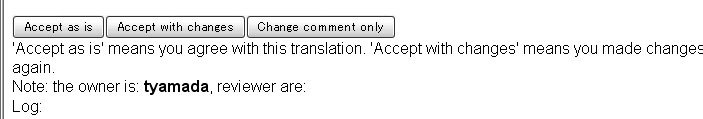
\includegraphics[scale=0.7]{image200906/ddtss145_mono.jpg}

\subsection{翻訳を新規に作成する}

翻訳を新規に作成する場合は Pending Translation から選択してください。
レビューの際と違うのは、選択肢が Abandon (翻訳を中止する)と Submit (翻訳
を確定しレビューにまわす)の二つになっている点です。

\subsection{debian-doc ML へのお誘い}

翻訳の内容に疑問があったり、相談が必要だと思ったり、レビューや修正で 
(小さくない) 変更があったら、debian-doc ML に流してください。

debian-doc ML の宛先は、\url{debian-doc@debian.or.jp}

参加方法は、\url{http://www.debian.or.jp/community/ml/openml.html#docML}


質問や相談はフリーフォーマットです。

レビューを依頼するときは、次のメール例を参考にしてください。

(メールの例)

\begin{commandline}
Subject: DDTSS レビュー icedax

xxxです。

xxxx さんが修正した icedax をレビューしました。


Short description

原文: Creates WAV files from audio CDs
訳文: オーディオ CD から WAV を生成する

Long description

原文:
icedax lets you digitally copy ("rip") audio tracks from a CD, avoiding
(略)

訳文:
icedax により、CD からディジタルでオーディオトラックのコピー ("リッピング")
(略)

用語を一部修正しました。
ディジタル->デジタル

修正後:
icedax により、CD からディジタルでオーディオトラックのコピー ("リッピング")
(略)

修正処理をしましたので、内容の確認をお願いします。
\end{commandline}


\subsection{debian-doc ML だけでレビューする}

「DDTSS をやる時間がないよ」という方は、
debian-doc ML に流れているレビューや翻訳完了のメールを確認して、
何か問題が見つけたらメールに返信してください。
きっと誰かが DDTSS に反映するでしょう。

\subsection{最後に}

DDTSSは仕組み上レビューが大量に必要になります。
多くの人が参加していることが前提になっています。
なので、翻訳が正しい内容なのかを利用者の視点でレビューしてくれると助かります。

%200909 kansai
\dancersection{GUIがついて格好良くなったreportbugを使ってみよう}{のがたじゅん}
\index{reportbug}
\index{bts}
\index{bug tracking system}

\subsection{はじめに}

Debianのバグ報告支援ツールreportbugが、バージョン3.99.0からGTK2を利用した
ユーザーインターフェースが使えるようになっていましたが、あまり知られていない
のでreportbugの使い方も兼ねて書いてみました。

\subsubsection{おわび}

「使ってみよう」とタイトルに書きましたが、実際にGTK2インターフェースで使
うとquerybtsがうまく動かず登録されたバグを表示することができなかったり、
戻るボタンで戻ると入力ができなかったりと不具合あります。ですので「使う」
には難しいところもありますが、とりあえずこんな感じということを知ってもら
えれば思います。

\subsection{reportbugとは}

Debianを使っていて発見したバグは、決められた書式にしたがって書いたメール
をDebianのバグ追跡システム(Bug Tracking System.通称BTS)に送ることによって
バグを報告することができます \footnote{バグレポートから参加するDebianパッ
ケージ開発 / 木下 達也 (あんどきゅめんてっど でびあん 2008年夏号)

\url{http://tokyodebian.alioth.debian.org/pdf/debianmeetingresume2008-natsu.pdf}}。ですがバグ報告に慣れていないと、決められた
書式でメールを書くことはもちろんのこと、バグ修正に必要なパッケージ情報な
どを洩れなく集めたりすることは大変なことです。

reportbugは、そういったバグ報告の負担を減らすためのツールで、バグ検索から、
バグ報告のためのパッケージ情報の収集、バグ登録に必要なメールの書式整形、
報告メールの送信まで行ってくれるツールです。

\subsection{reportbugのインストール}

Debianインストール時に「標準システム」を選択すると、reportbugはインストー
ルされますが、GTK2や端末上でのメニューインターフェースに必要なRecommends
やSuggestsパッケージはインストールされないので、改めてreportbugをインストー
ルします。

\begin{commandline}
 # apt-get update
 # apt-get remove reportbug
 # apt-get -o APT::Install-Suggests=true --install-recommends -y install reportbug
\end{commandline}

まどろっこしいことをしていますが、すでにインストールされたパッケージの
RecommendsやSuggestsパッケージをスマートにインストールするにはどうしたら
いんでしょうか?

\subsection{reportbugを起動}

reportbugを起動します。

デスクトップのメニュー([アプリケーション]→[システムメ
ニュー]→[reportbug])から起動すると、GTK2インターフェースのウィンドウが開
きます。端末から起動するとメッセージが表示されます。

\begin{commandline}
 $ reportbug 
\end{commandline}

\begin{figure}[h]
 
\includegraphics[scale=0.5]{image200909/reportbug-initial_mono.png}
 \caption[reportbugのGTK2インターフェース]{reportbugのGTK2インターフェース}
\end{figure}

\subsection{初期設定}
reportbugを初めて起動すると、reportbugを使うための設定を尋ねられます。
初期設定の途中、バグ報告メールを送信するためのメール環境について尋ねられ
るので、あらかじめメールの設定を確認しておいてください。
設定例では、Gmailを使っていることを前提に話を進めます。

\begin{itemize}
 \item 参考: その他のメール クライアントの設定 - Gmail ヘルプ:

\url{http://mail.google.com/support/bin/answer.py?hl=jp&answer=13287}
\end{itemize}

\begin{commandline}
Welcome to reportbug! Since it looks like this is the first time you have used reportbug, we are configuring its behavior.

These settings will be saved to the file "/home/hoge/.reportbugrc", which you will be free to edit further.                
Please choose the default operating mode for reportbug.                                                                   

1 novice    Offer simple prompts, bypassing technical questions.

2 standard  Offer more extensive prompts, including asking about things that a moderately sophisticated user would be
            expected to know about Debian.                                                                           

3 advanced  Like standard, but assumes you know a bit more about Debian, including "incoming".

4 expert    Bypass most handholding measures and preliminary triage routines. This mode should not be used by people
            unfamiliar with Debian's policies and operating procedures.                                             

Select mode: [novice] 
\end{commandline}

ウェルカムメッセージと設定は~/.reportbugrcに保存されていますと二つのお知
らせの後、reportbugで使うモードについて尋ねています。とりあえずは細かいこ
とよりバグ報告だけに絞りたいので、noviceのままでよいでしょう。

\newpage

\begin{commandline}
Please choose the default interface for reportbug.

1 text   A text-oriented console user interface

2 gtk2   A graphical (GTK+) user interface.

3 urwid  A menu-based console user interface

Select interface: 2
\end{commandline}

どのユーザーインターフェースを使うか選択します。
今回はテーマにそってgtk2を選びました。実際に使うとなるとurwidが使いやす
いと思います。

\begin{commandline}
Will reportbug often have direct Internet access? (You should answer yes to this question unless you know what you are doing
and plan to check whether duplicate reports have been filed via some other channel.) [Y|n|q|?]?
\end{commandline}

インターネットに接続しているかですが、おそらくほとんどの人は接続している
と思うので、yと答えます。

\begin{commandline}
What real name should be used for sending bug reports?
[Hogewo HOGETA]>
\end{commandline}

バグ報告に使う名前を設定します。

\begin{commandline}
Which of your email addresses should be used when sending bug reports? (Note that this address will be visible in the bug
tracking system, so you may want to use a webmail address or another address with good spam filtering capabilities.)
[example@gmail.com]>
\end{commandline}

バグ報告に使うメールアドレスを設定します。
ここで気をつけないといけないことは、ここで設定したメールアドレスはバグ報
告をすると公開されます。あまり公開したくないメールアドレスは設定しないほ
うがよいでしょう。

\begin{commandline}
Do you have a "mail transport agent" (MTA) like Exim, Postfix or SSMTP configured on this computer to send mail to the
Internet? [Y|n|q|?]? n
\end{commandline}

バグ報告をするマシンでメールサーバーが動いているか尋ねています。
GmailのSMTPサーバーを使って送信するので、ここではnと答えます。

\begin{commandline}
Please enter the name of your SMTP host.  Usually it's called something
 like "mail.example.org" or "smtp.example.org".
If you need to use a different port than default, use the <host>:<port> alternative format.

Just press ENTER if you don't have one or don't know.
> smtp.gmail.com:587
\end{commandline}

送信するSMTPサーバーを登録します。
GmailのSMTPサーバーのアドレスはsmtp.gmail.com、ポート番号は587なので、
smtp.gmail.com:587と登録します。

\begin{commandline}
If you need to use a user name to send email via "smtp.gmail.com:587" on your computer, please enter that user name. Just
press ENTER if you don't need a user name.
> nogajun@gmail.com
\end{commandline}

SMTPサーバーを利用するためのユーザー名を登録します。
GmailのSMTPサーバーを使うにはドメイン名も含めたユーザー名が必要なので、<ユーザー
名>@gmail.comと登録します。

\begin{commandline}
Does your SMTP host require TLS authentication? [y|N|q|?]? y
\end{commandline}

SMTPはTLSを使うかの問いについては、Gmailでは必要なのでyと答えます。

\begin{commandline}
Please enter the name of your proxy server. It should only use this parameter if you are behind a firewall. The PROXY
argument should be formatted as a valid HTTP URL, including (if necessary) a port number; for example,
http://192.168.1.1:3128/. Just press ENTER if you don't have one or don't know.
>
\end{commandline}
Proxyについて尋ねています。使っていれば設定します。使っていなければ空のまま
でEnterキーを押します。

\begin{commandline}
Default preferences file written. To reconfigure, re-run reportbug with the "--configure" option.
\end{commandline}
初期設定が終わりました。もう一度、設定をやり直したいときは、--configureオ
プションをつけて起動するとやり直すことができます。

\subsection{reportbugを使ってみる}

 
\includegraphics[scale=0.5]{image200909/reportbug-1_mono.png}

起動するとこんな感じです。ウィザード形式なのでわかりやすいと思います。

 
\includegraphics[scale=0.5]{image200909/reportbug-2_mono.png}

バグを見つけたパッケージ名を入力します。パッケージ名の頭を何文字か入力す
ると、インストールされているパッケージの候補を表示してくれます。

 
\includegraphics[scale=0.5]{image200909/reportbug-8_mono.png}

パッケージ名の入力でotherと入力するとこの画面になります。これは擬似パッケー
ジの一覧です。パッケージ以外に見つけたDebianに関連する問題を擬似パッケー
ジのバグとして登録します。

\begin{itemize}
 \item Debian -- Debian バグ追跡システム - 擬似パッケージ:

\url{http://www.debian.org/Bugs/pseudo-packages.ja.html}

\end{itemize}


\includegraphics[scale=0.5]{image200909/reportbug-3_mono.png}

本来ならばここに登録されたバグが表示されて、今から登録しようとしたバグが
すでに登録済みかどうか確認できるのですが、GTK2インターフェースだと
querybtsがうまく動かなくて(\#432178)、ダブルクリックをしても何も表示され
ません。残念。


\includegraphics[scale=0.5]{image200909/reportbug-4_mono.png}

バグがまだ登録されていなかったとして次に進むと、バグを登録する画面に入り
ます。ここではバグの概要を簡潔に書きます。

\includegraphics[scale=0.5]{image200909/reportbug-5_mono.png}

バグの種類を指定します。種類はCriticalやSeriousのような深刻なものから、提
案のWhishlistまであります。通常はnormalでいいと思います。

\includegraphics[scale=0.5]{image200909/reportbug-6_mono.png}

ここでは、バグの内容を書きます。
スクリーンショットのために適当なことを書いて撮っていたのでSubjectは消して
いますが、通常はSubjectの箇所に上で書いたバグの概要が入っています。

\includegraphics[scale=0.5]{image200909/reportbug-7_mono.png}

バグの内容を書き終わって進むと、この画面になります。

この時点ではまだメールは送信されてません。問題がないと思うなら、Submit
the bug report via email.ボタンを押して送信します。いや、もう少しだけ確認
したい、とりあえず下書きで保存して続きは後で書く、ファイルを添付したいな
どあれば、それぞれのボタンを押して終了します。

\subsection{まとめ}
reportbugを使うと簡単にバグ報告ができるので、みんなバグを見つけたらバグ報
告しよう。

あと、のがじゅんはさっさと仕事をしよう。実例をあげて説明しようと目星をつ
けてたパッケージを見たら、バグが修正されてて困った困った。

\subsection{参考資料}

\begin{itemize}
 \item Debian JP Project - バグ報告:

\url{http://www.debian.or.jp/community/bugreport.html}

\item Debian -- Debian BTS - バグを報告する:

\url{http://www.debian.org/Bugs/Reporting.ja.html}

\item MC-MPI Debian 公式パッケージへの道 / 藤澤 徹

第52回東京エリアDebian勉強会 2009年5月勉強会 配布資料

\url{http://tokyodebian.alioth.debian.org/pdf/debianmeetingresume200905.pdf}

\end{itemize}

%-------------------------------
\dancersection{Debian パッケージの作り方。最初から最後まで}{佐々木洋平}
\index{ぱっけーじさくせい@パッケージ作成}

\subsection{はじめに}

...なんて{\bf 大それた}タイトルなんでしょう..%
私事で忙しくて訂正できなかった訳ですが、 我ながら恥ずしいです。

さて、 佐々木のパッケージ作成遍歴は以下の通りです:
\begin{enumerate}
      \item 売り物ソフトウェアを dpkg で管理するために弄り始める
      \item 自分達の作っているソフトウェアの deb パッケージを作成し始める。
      \item どうせなら本家に... $\leftarrow$ イマココ
\end{enumerate}
今日のお話は、 これらを踏まえての「パッケージ作成最初から最後まで」です。
ここでは「最初」を「ソースの取得」、「最後」を「lintian \& piuparts clean」
とします。 
個々の How to、 特に一番ハマりやすい {\tt debian/rules}については
時間の紙面の都合上参考文献へのポインタを示すに留めます。 是非質問して下さい。
\index{debian/rules}

\subsection{Package}

コンパイル後のソフトウェアなどをすぐ利用できる形に
まとめたものをバイナリパッケージと呼びます。 
%
Debian では拡張子が {\tt .deb} のファイルがこれにあたります。
%
我々は普段 {\tt apt-get}や{\tt aptitude} を利用して、 バイナリパッケージ
を導入/更新/削除したりしています。
%
バイナリパッケージは制御情報とデータを {\tt tar.gz}に圧縮し、 
バージョン情報とともに {\tt ar(1)} でまとめたものです。
%
これらは非常に一般的なコマンドですから、
バイナリパッケージを展開するだけならば多くのシステムで可能です。

バイナリパッケージに対して、 
これを作成するための素材をまとめたものをソースパッケージと言います。 
%
これは二つないし三つのファイルからなります:
\begin{itemize}
      \item オリジナルのソース一式({\tt .orig.tar.gz})
      \item パッケージの情報({\tt .dsc}))
      \item バイナリパッケージを作成するための変更({\tt .diff.gz})
    \begin{itemize}
          \item オリジナルのソースが無い場合
        (Debian 固有のパッケージ等)の場合は存在しない。
    \end{itemize}
\end{itemize}
ソースパッケージは
導入したり削除したりする性質のパッケージではありません。  
%
目的はバイナリパッケージの作成にあります。 
%
Debian が提供しているバイナリパッケージには、 
対応するソースパッケージが必ず存在しており、 
必要に応じてソースパッケージを取得してバイナリパッケージを構築する
ことができます。

\subsubsection{deb package inside}

\index{dpkg-deb}
{\tt dpkg-deb} コマンドを利用して、 実際にパッケージを展開してみましょう。
%
\index{rabbit}
例えば rabbit\footnote{%
RD や Wiki フォーマットで記述したテキストをベースにした
プレゼンテーションツール。 この間 unstable に入りました!!} 
%
というパッケージの deb ファイルを展開してみると...
\begin{commandline}
  % dpkg-deb -x rabbit_0.6.1-1_all.deb rabbit
                 (rabbit というパッケージを rabbit というディレクトリに展開)
  % dpkg-deb -e rabbit_0.6.1-1_all.deb rabbit/DEBIAN        
                 (rabbit パッケージの制御情報を rabbit/DEBIAN に展開)
  % cd rabbit ls 
  DEBIAN/  usr/
  % tree 
  .
  |-- DEBIAN
  |   |-- control
  |   |-- md5sums
  |   `-- preinst
  `-- usr
      |-- bin
      |   |-- rabbit
-------- snip ---------------
      |   `-- rabbit-theme-manager
      |-- lib
      |   `-- ruby
      |       `-- 1.8
      |           |-- rabbit
-------- snip ---------------
      |         
      `-- share
          |-- doc
          |   `-- rabbit
          |       |-- NEWS.en.gz -> changelog.gz
-------- snip ---------------
          |       |-- README.Debian
          |       |-- README.en.gz
          |       |-- README.ja.gz
          |       |-- changelog.Debian.gz
          |       |-- changelog.gz
-------- snip ---------------
          ...
179 directories, 575 files
\end{commandline}
パッケージの制御情報は DEBIAN以下に展開しました。 
{\tt rabbit} の場合、 
\begin{commandline}
  % ls -R DEBIAN
  DEBIAN:
  control  md5sums  preinst*
\end{commandline}
の三つからなります。 これらは
\begin{description}
      \item[control] 
    メンテナの名前、 
    対応するソースパッケージ名、 依存関係などが記述されたファイル
      \item[md5sums]
    提供される各ファイルの md5 checksum
      \item[preinst]
    インストール作業の前に実行される hook シェルスクリプト。
    パッケージによっては、 
    {\tt preinst} 以外に
    {\tt postinst}、 {\tt prerm}、{\tt postrm} などが存在します。
\end{description}


パッケージのデータは {\tt usr} 以下に展開しました。
%
deb パッケージを導入した際には、 これらは {\tt /usr} 以下に展開されます。

というわけで上記構成になったディレクトリツリーを用意して
tar.gz で圧縮したりするとバイナリパッケージができあがります。

\subsubsection{余談: dpkg-deb でパッケージを再構築}
\label{subsubseclab:余談}

売り物の(ソースが取得できない)ソフトウェアを
Debian のパッケージシステムで管理したい
時に佐々木がよくやる手段は
\begin{itemize}
      \item {\tt alien} で rpm を deb に変換
      \item 上記 {\tt dpkg-deb -e|-x} でファイルを展開
      \item 適切に配置、 修正
      \item {\tt dpkg-deb -b} で再アーカイブ
\end{itemize}
として、 似非パッケージを作成することです。
当然配布はできませんが%
\footnote{売り物って rpm ばっかりです。Ubuntu のおかげで大分減りましたが。}
例として、 大昔の Intel Compiler Ver.8 のパッケージ作成は以下の様にやって
いました。
\begin{commandline}
 % tar xvzf l_cc_pc_8.1.028.tar.gz
 % cd l_cc_pc_8.1.028
 % rm -rf *64*
 % sudo alien *.rpm
 % rm *.rpm
 % sudo chown $USER *.deb
 % mkdir tmp
 % dpkg-deb -e intel-icc8_8.1-29_i386.deb tmp/DEBIAN
 % dpkg-deb -x intel-icc8_8.1-29_i386.deb tmp/
 % echo DESTINATION=/opt/`ls tmp/opt` >> tmp/DEBIAN/postinst
 % cat <<EOF >> tmp/DEBIAN/postinst
  for FILE in $(find $DESTINATION/bin/ -regex \
     '.*[ei](cc|fort|fc|cpc)$\|.*cfg$\|.*pcl$\|.*vars[^/]*.c?sh$' \
     2> /dev/null) do
      sed s@\@$DESTINATION@g $FILE > ${FILE}.abs
      mv ${FILE}.abs $FILE
      chmod 755 $FILE
  done
  for FILE in $(find $DESTINATION/bin/ -regex '.*[ei]cc' 2> /dev/null) do
      sed s@\@$DESTINATION@g $FILE > ${FILE}.abs
      mv ${FILE}.abs $FILE
      chmod 755 $FILE
  done
  for FILE in $(find $DESTINATION/bin/ -regex '.*[ei]cpc' 2> /dev/null) do
      sed s@\@$DESTINATION@g $FILE > ${FILE}.abs
      mv ${FILE}.abs $FILE
      chmod 755 $FILE
  done
  for FILE in $(find $DESTINATION/bin/ -regex '.*[ei]fort' 2> /dev/null) do
      sed s@\@$DESTINATION@g $FILE > ${FILE}.abs
      mv ${FILE}.abs $FILE
      chmod 755 $FILE
  done
  for FILE in $(find $DESTINATION/bin/ -regex '.*[ei]fc' 2> /dev/null) do
      sed s@\@$DESTINATION@g $FILE > ${FILE}.abs
      mv ${FILE}.abs $FILE
      chmod 755 $FILE
  done
 EOF
 % dpkg-deb -b tmp intel-icc8_8.1-29_i386.deb
 % dpkg -i intel-icc8_8.1-29_i386.deb
 % dpkg -i intel-iidb8_8.1-46_i386.deb
 % dpkg -i --force-overwrite intel-isubh8_8.1-29_i386.deb
\end{commandline}
最近は Intel Compiler に愛がない\footnote{%
マイナーバージョン上がる度にディレクトリ構成がコロコロ変わるので
つきあいきれなくなりました}
のでやっていませんが。

\subsection{パッケージ作成}

さて、 単にバイナリパッケージを作成するだけならば
前小節(\ref{subsubseclab:余談})で示した通り
\begin{itemize}
      \item DEBIAN 以下に control、 md5sums、 必要ならば hook スクリプト
      \item パッケージとして / 以下に展開したいディレクトリ構成に揃えた
    ファイル群
\end{itemize}
を作成して dpkg-deb でまとめれば良いだけです。 
%
ですが、 あんまり一般的ではありませんね。
%
以下では、 {\tt GNU hello} を例に\footnote{「またー?」とか言わないこと}、 
実際に配布まで含めたパッケージ作成方法について述べてみます。

\subsubsection{前準備} 

\paragraph{環境変数の設定}
パッケージメンテナの名前とメールアドレスを環境変数に設定します:
\begin{commandline}
DEBFULLNAME="Youhei SASAKI"; export DEBFULLNAME
DEBEMAIL=uwabami@gfd-dennou.org ; export DEBEMAIL
\end{commandline}
配布も考えているなら GPG 鍵の記述に合わせておくと良いと思います。

\paragraph{最低限必要なパッケージの導入}

{\tt build-essential} メタパッケージを導入しておきます。 このパッケージ
はdeb パッケージを構築するのに最低限必要となるパッケージを導入するメタ
パッケージです。 
%
具体的には
\begin{enumerate}
      \item {\tt libc6-dev} $|$ {\tt libc-dev}
      \item {\tt g++}
      \item {\tt make}
      \item {\tt dpkg-dev}
\end{enumerate}
とこれに依存する幾つかのファイルが導入されます
\footnote{{\tt dpkg-dev} が {\tt make} に依存しているので、 
なんか変な気分ですが、 正しいんですよね? きっと…}。

\begin{commandline}
% apt-cache show build-essential
Package: build-essential
Priority: optional
Section: devel
Installed-Size: 48
Maintainer: Matthias Klose <doko@debian.org>
Architecture: amd64
Version: 11.4
Depends: libc6-dev | libc-dev, g++ (>= 4:4.3.1), make, dpkg-dev (>= 1.13.5)
Filename: pool/main/b/build-essential/build-essential_11.4_amd64.deb
Size: 7126
MD5sum: 86a942017ad93721c91212398a828a0c
SHA1: 5ac2ba90444e1eaed96b2163389a8812eb107b01
SHA256: 3dbd2e6b4e998412a6ad4d32b242523559b536168bcce7f227c7ce30256808a5
Description: Informational list of build-essential packages
 If you do not plan to build Debian packages, you don't need this
 package.  Starting with dpkg (>= 1.14.18) this package is required
 for building Debian packages.
 .
 This package contains an informational list of packages which are
 considered essential for building Debian packages.  This package also
 depends on the packages on that list, to make it easy to have the
 build-essential packages installed.
 .
----- snip -----
% sudo aptitude install build-essential
\end{commandline}

\paragraph{ソースの取得、 確認}
動かないソフトウェアをパッケージ化するのは大変ですよね?  事前にソースを
取得して動作確認しておくと良いでしょう。  また「動作させるために patch
を書いた!」という猛者は、 そのパッチを保管しておくと幸せになれるかもしれません。

{\tt GNU hello} は次の URL から取得できます。
\url{http://www.gnu.org/software/hello/}

{\tt GNU hello} は {\tt configure ; make ; make install} で導入する
ソフトウェアです。 実際に configure を動かしてみます。
\begin{commandline}
% cd hello-2.4
% ./configure 
...
\end{commandline}
エラーがでなければこれで終了です。
もし{\tt ./configure} が必要なファイルを探せずエラー終了する場合には、
{\tt apt-file} コマンドで必要なファイルを提供している
Debian パッケージを探してみましょう。
\begin{commandline}
% sudo aptitude install apt-file
% sudo apt-file update
% apt-file search [file 名]
\end{commandline}
足りないファイルを導入したら、 もう一度 {\tt ./configure} を走らせます。
これをくりかえして、 必要なファイルを導入していきます。

無事 {\tt ./configure} が通るようになったら {\bf make} を実行してみます。
\begin{commandline}
% make 
make all-recursive
make[1]: Entering directory `/home/uwabami/Desktop/hello-2.4'
Making all in contrib
make[2]: Entering directory `/home/uwabami/Desktop/hello-2.4/contrib'
make[2]: Nothing to be done for `all'.
make[2]: Leaving directory `/home/uwabami/Desktop/hello-2.4/contrib'
...
make[2]: Entering directory `/home/uwabami/Desktop/hello-2.4'
make[2]: Leaving directory `/home/uwabami/Desktop/hello-2.4'
make[1]: Leaving directory `/home/uwabami/Desktop/hello-2.4'
\end{commandline}
コンパイルも正常に終了したので、試しに実行してみます。
\begin{commandline}
% ./src/hello
% ./src/hello -t
% ./src/hello -g "Good Night。.."
\end{commandline}
ここまでがパッケージ作成前の動作確認作業です。

実際に配布するためのパッケージを作成する場合には、 
動作確認以外にも Copyright や License を確認しておくべきです。

\subsubsection{パッケージ作成}

\paragraph{雛形の作成}

{\tt dh\_make}コマンドでパッケージの雛形を作成します。
{\tt dh\_make}は、{\tt dh-make}パッケージで提供されていますので、
これを導入します
\begin{commandline}
% sudo aptitude install dh-make
% dh_make --help
dh_make - prepare Debian packaging for an original source archive, version 0.50

Copyright (C) 1998-2009 Craig Small <csmall@debian.org>
This is free software; see the source for copying conditions.  There is NO
warranty; not even for MERCHANTABILITY or FITNESS FOR A PARTICULAR PURPOSE.
  Usage: dh_make [options]
  -c, --copyright <type>    use <type> of license in copyright file
                            (apache|artistic|bsd|gpl|gpl2|gpl3|lgpl|lgpl2|lgpl3)
      --dpatch              using dpatch to maintain patches
      --quilt               using quilt to maintain patches
  -e, --email <address>     use <address> as the maintainer e-mail address
  -n, --native              the program is Debian native, don't generate .orig
  -f, --file <file>         specify file to use as the original source archive
  -r, --createorig          make a copy for the original source archive
  -s, --single              set package class to single
  -i, --indep                           set package class to arch-independent
  -m, --multi               set package class to multiple binary
  -l, --library             set package class to library
  -k, --kmod                set package class to kernel module
      --kpatch              set package class to kernel patch
  -b, --cdbs                set package class to cdbs
  -a, --addmissing          reprocess package and add missing files
  -t, --templates <dir>      apply customizing templates in <dir>
  -d  --defaultless         skip the default debian and package class templates
  -o, --overlay <dir>       reprocess package using template in <dir>
  -p, --packagename <name>  force package name to be <name>
  -h, --help                display this help screen and exit
  -v, --version             show the version and exit

By Craig Small <csmall@debian.org>
Based on deb-make by Christoph Lameter <clameter@debian.org>.
Custom template support by Bruce Sass <bmsass@shaw.ca>.
\end{commandline}

ここでは
\begin{description}
      \item[--createorig, -r] 
    オリジナルのソースファイル(.orig.tar.gz)を作成する
      \item[--copyright gpl, -c gpl] ソースのライセンスが gpl3 なので。
    ライセンスが代表的なモノの場合、
    指定しておくと雛形の時点で結構できあがっていて、 非常に楽です。
      \item[--single,  -s] シングルバイナリのパッケージを作成します。
    ライブラリの場合には {\tt -l} としてすると良いでしょう。
      \item[--cdbs, -b] CDBS(後述)を使用するので指定します。
    \item[--quilt, --dpatch]
  パッチを当てることが決まっているのであれば
  {\tt --dpatch} もしくは{\tt --quilt} を指定しておくと良いでしょう。
  今回は指定しません。
\end{description}
以下のコマンドを実行します。
\begin{commandline}
% dh_make --createorig --copyright gpl --single --cdbs
(もしくは)
% dh_make -r -c gpl -s -b 
\end{commandline}
  
実行すると以下のようなメッセージが表示されるので、確認して Enter を押します。
\begin{commandline}
Maintainer name : Youhei SASAKI
Email-Address   : uwabami@gfd-dennou.org
Date            : Sun, 25 Oct 2009 00:08:43 +0900
Package Name    : hello
Version         : 2.4
License         : gpl3
Using dpatch    : no
Using quilt     : no
Type of Package : cdbs
Hit <enter> to confirm:
\end{commandline}
うまく動作すると、{\tt debian} ディレクトリができ、このディレクトリ
以下に雛形({\tt .ex, .EX})ができます。
debian ディレクトリは以下のような状態になっています。
\begin{commandline}
.
|-- README.Debian        (パッケージの README)
|-- changelog            (パッケージのチェンジログ)
|-- compat               (パッケージのバージョン)
|-- control              (パッケージ情報)
|-- copyright            (パッケージのコピーライト情報)
|-- cron.d.ex            (パッケージで cron を使う場合の設定ファイル)
|-- dirs                 (パッケージでデータを配置するディレクトリ名の設定)
|-- docs                 (パッケージに含めるドキュメントファイルを指定する)
|-- emacsen-install.ex   (emacs 用設定ファイル)
|-- emacsen-remove.ex    (emacs 用設定ファイル)
|-- emacsen-startup.ex   (emacs 用設定ファイル)
|-- hello.default.ex     (パッケージで debfonf を使う場合の設定ファイル)
|-- hello.doc-base.EX    (パッケージで doc-base を使う場合の設定ファイル)
|-- init.d.ex            (パッケージで init.d を使う場合の設定ファイル)
|-- init.d.lsb.ex        (パッケージで init.d を使う場合の設定ファイル)
|-- manpage.1.ex         (manpage の雛形)
|-- manpage.sgml.ex      (manpage の雛形)
|-- manpage.xml.ex       (manpage の雛形)
|-- menu.ex              (メニューの雛形)
|-- postinst.ex          (postinstメンテナファイルの雛形)
|-- postrm.ex            (postrmメンテナファイルの雛形)
|-- preinst.ex           (preinstメンテナファイルの雛形)
|-- prerm.ex             (prermメンテナファイルの雛形)
|-- rules                (パッケージビルドスクリプト)
`-- watch.ex             (アップストリームチェック用ファイル)
\end{commandline}

ちなみにパッケージを作成する場合には{\bf このディレクトリの中以外は触りません}。
オリジナルのソースに変更を加える場合には
{\tt quilt} や {\tt dpatch} 等のパッチシステムを利用すると良いでしょう。

今回はおもむろに {\tt .ex, .EX} を削除します。
\begin{commandline}
% rm -f debian/*.ex debian/*.EX
\end{commandline}
\paragraph{CDBS}

パッケージの実際の構築は {\tt debian/rules} で行なわれます。
{\tt debian/rules} はいわゆる {\tt Makefile} ですので、 make の文法で
必要となる設定を行なっていきます。

{\tt GNU hello} は
./configure ; make ; make install で install しますので
この場合は {\tt cdbs} を使用した方が幸せになれます%
\footnote{%
 debhelper 7 の魔法の様な rules も凄いですが、 まだ使いこなせない...}。
{\tt dh\_make} に {\tt -b} を指定した場合、 {\tt debian/rules} は次の様に
なっています。
\begin{commandline}
#!/usr/bin/make -f

include /usr/share/cdbs/1/rules/debhelper.mk
include /usr/share/cdbs/1/class/autotools.mk


# Add here any variable or target overrides you need.
\end{commandline}
include されているのは
\begin{itemize}
      \item バイナリパッケージの作成支援のためのコマンドである
    {\tt debhelper} を必要なタイミングで呼びだす。
    \item パッケージの作成に autotools を使う
\end{itemize}
という命令セットです。

CDBS の詳細については、 
例えば\cite{CDBS1st}、 \cite{CDBS ギャラリ}、 \cite{CDBS doc}を参照下さい。
\index{cdbs}

\paragraph{rules の調整}

ここで一旦バイナリパッケージを作成してみましょう。
\begin{commandline}
  % sudo aptitude install fakeroot
  % fakeroot debian/rules binary
  ...
\end{commandline}

rules の binary ターゲットを実行することで、 
ソースの一つ上のディレクトリにバイナリパッケージが作成されます。
この時点ではバイナリパッケージには見向きもせず
{\tt debian} ディレクトリの下に生成される
{\tt debian/hello} 以下を確認します。
\begin{commandline}
|-- DEBIAN
|   |-- control
|   `-- md5sums
`-- usr
    |-- local
    |   |-- bin
    |   |   `-- hello
    |   `-- share
    |       |-- info
    |       |   `-- hello.info
    |       |-- locale
    |       |   |-- bg
    |       |   |   `-- LC_MESSAGES
    |       |   |       `-- hello.mo
--------- snip -------------------
...
103 directories, 61 files
\end{commandline}
{\tt hello} が {\tt /usr/local/bin} に install されています。
これは変ですよね? build 時のlog を注意深く見ていると、 {\tt configure} 
実行時に {\tt --prefix} が指定されておらず、 {\tt /usr/local} 以下に
設定されています。

よって{\tt cdbs} に対して {\tt configure} 実行時に {\tt --prefix=/usr}
を指定するようにします。

\begin{commandline}
#!/usr/bin/make -f

include /usr/share/cdbs/1/rules/debhelper.mk
include /usr/share/cdbs/1/class/autotools.mk

DEB_CONFIGURE_EXTRA_FLAGS:= --prefix=/usr

\end{commandline}
もういちど {\tt fakeroot debian/rules binary} を実行します。
これを繰り返して、 ファイルが望んだ配置になるまで {\tt debian/rules} を
修正していきます。


\paragraph{制御情報の編集}

具体的には 
\begin{enumerate}
      \item {\tt debian/control}
      \item {\tt debian/changelog}
      \item {\tt debian/copyright}
\end{enumerate}
の三つです。
特記事項が無いならば {\tt debian/README.Debian} は削除しても良いでしょう。

control の例:
\begin{commandline}
Source: hello
Section: devel
Priority: optional
Maintainer: Youhei SASAKI <uwabami@gfd-dennou.org>
Build-Depends: cdbs, debhelper (>= 7), autotools-dev
Standards-Version: 3.8.3
Homepage: http://www.gnu.org/software/hello

Package: hello
Architecture: any
Depends: ${shlibs:Depends}, ${misc:Depends}
Description: The classic greeting, and a good example
 The GNU hello program produces a familiar, friendly greeting.  It
 allows non-programmers to use a classic computer science tool which
 would otherwise be unavailable to them.
 .
 Seriously, though: this is an example of how to do a Debian package.
 It is the Debian version of the GNU Project's `hello world' program
 (which is itself an example for the GNU Project).
\end{commandline}

changelog の例:
\begin{commandline}
% cat debian/changelog    
hello (2.4-1) unstable; urgency=low

  * Initial release

 -- Youhei SASAKI <uwabami@gfd-dennou.org>  Sun, 25 Oct 2009 00:08:43 +0900

\end{commandline}
雛形には ITP のバグ番号を記述するところがあります。
ITP している場合には埋めておくと良いと思います。

copyright の例:
\begin{commandline}
This work was packaged for Debian by:

    Youhei SASAKI <uwabami@gfd-dennou.org> on Sun, 25 Oct 2009 00:08:43 +0900

It was downloaded from:

    http://www.gnu.org/software/hello/

Upstream Author:

Authors of GNU Hello.

  Copyright (C) 1999, 2005, 2006 Free Software Foundation, Inc.

  Copying and distribution of this file, with or without modification,
  are permitted in any medium without royalty provided the copyright
  notice and this notice are preserved.

The following contributions warranted legal paper exchanges with the
Free Software Foundation.  See also the ChangeLog and THANKS files.

Mike Haertel
David MacKenzie
Jan Brittenson
Roland McGrath
Charles Hannum
Bruce Korb              hello.c, configure.ac.
Karl Eichwalder         all files.
Karl Berry              all files.
The King                releases.

License:

    This program is free software: you can redistribute it and/or modify
    it under the terms of the GNU General Public License as published by
    the Free Software Foundation, either version 3 of the License, or
    (at your option) any later version.

    This package is distributed in the hope that it will be useful,
    but WITHOUT ANY WARRANTY; without even the implied warranty of
    MERCHANTABILITY or FITNESS FOR A PARTICULAR PURPOSE.  See the
    GNU General Public License for more details.

    You should have received a copy of the GNU General Public License
    along with this program.  If not, see <http://www.gnu.org/licenses/>.

On Debian systems, the complete text of the GNU General
Public License version 3 can be found in `/usr/share/common-licenses/GPL-3'.

The Debian packaging is:

    Copyright (C) 2009 Youhei SASAKI <uwabami@gfd-dennou.org>

and is licensed under the GPL version 3, see above.
\end{commandline}
ソースに AUTHORS とか COPYING とかある場合には、 編集が非常に楽ですね。

\paragraph{debuild, lintian}

バイナリパッケージとソースパッケージの作成、 
パッケージのポリシー違反の確認を行ないます。
{\tt devscripts}と{\tt linitian} を導入します。
\begin{commandline}
% sudo aptitude install debuild lintian
\end{commandline}
その後、 {\tt debuild} コマンドを実行します:
\begin{commandline}
% debuild -rfakeroot -uc -us
...
W: hello source: configure-generated-file-in-source config.status
W: hello source: configure-generated-file-in-source config.log
W: hello: new-package-should-close-itp-bug
Finished running lintian.
\end{commandline}
{\tt -uc}、 {\tt -us} は GPG サインをしない設定です。GPG でサインする場合には
このオプションを省略して下さい。

最後に出てきたのが {\tt lintian }によるチェック結果です。
これを解決しましょう。最後の ITP は今回しょうがないですが、
上の二つは config.status、 config.log を 
clean ターゲットが呼ばれた時に消去するようにすれば良いのです
\begin{commandline}
% cat debian/rules
#!/usr/bin/make -f

include /usr/share/cdbs/1/rules/debhelper.mk
include /usr/share/cdbs/1/class/autotools.mk

DEB_CONFIGURE_EXTRA_FLAGS:= --prefix=/usr

clean::
	rm -f config.status config.log
\end{commandline}
この後でもう一度 debuild してみます。
\begin{commandline}
% debuild -rfakeroot -uc -us
...
dpkg-deb: `../hello_2.4-1_amd64.deb' にパッケージ `hello' を構築しています。
 dpkg-genchanges  >../hello_2.4-1_amd64.changes
dpkg-genchanges: including full source code in upload
dpkg-buildpackage: full upload (original source is included)
Now running lintian...
W: hello: new-package-should-close-itp-bug
Finished running lintian.
\end{commandline}
ITP したならば、 {\tt debian/changelog} に ITP の番号を書いておくと
最後の warning も消せますね。


これでオシマイ。 メデタシメデタシ…ではありません。

\subsection{パッケージのビルド・インストールテスト}

まず、 ビルドテストを行ないます。
ビルドテストは大雑把に言えば、 
ソースパッケージを元に
\begin{itemize}
      \item {\tt debian/control} の内容を元に
    構築に必要な他のパッケージを導入し
      \item {\tt debian/rules} を実行してバイナリパッケージを作成し
      \item {\tt lintian } に怒られないパッケージができあがる
\end{itemize}
ことをテストします。

ビルドテストには {\tt pbuilder} を使用します。
{\tt pbuilder} は必要最小限の Debian パッケージが導入された
環境の tar.gz を用いて、 
パッケージのビルド時にその tar.gz を展開し
chroot してパッケージの作成を行ないます。

\index{pbuilder}
まずは pbuilder 環境を導入します%
\begin{commandline}
% sudo aptitude install pbuilder
% sudo pbuilder  --create --distribution sid
\end{commandline}
ちょっと時間がかかりますが気長に待ちます。
これによって /var/cache/pbuilder/base.tgz が生成されます。
これを使用してビルドテストを行ないます。
\begin{commandline}
% sudo pbuilder --build --distribution sid --basetgz /var/cache/pbuilder/base.tgz hello_2.4-1.dsc
\end{commandline}
無事に build テストが通りましたか? きちんとパッケージができているなら
{\tt /var/cache/pbuilder/result} 以下にパッケージが置かれています。

さてパッケージのビルドテストが通ったら、 
次はインストール/アンインストールテストです。
これには {\tt piuparts}パッケージを使用します。
\begin{commandline}
% sudo aptitude install piuparts    
\end{commandline}
\index{piuparts}

piuparts も pbuilder と同様に最低限の環境からインストール
/アンインストールテストを実行します。 pbuilder で作成した base.tgz を
使用してみましょう。
\begin{commandline}
% sudo piuparts -d sid -b /var/cache/pbuilder/base.tgz hello_2.4-1_amd64.deb
...
0m50.1s DEBUG: No broken symlinks as far as we can find.
0m51.3s INFO: PASS: Installation, upgrade and purging tests.
0m51.3s DEBUG: Starting command: ['chroot', '/tmp/tmpZ2-nup', 'umount', '/proc']
0m51.3s DEBUG: Command ok: ['chroot', '/tmp/tmpZ2-nup', 'umount', '/proc']
0m51.7s DEBUG: Removed directory tree at /tmp/tmpZ2-nup
0m51.7s INFO: PASS: All tests.
0m51.7s INFO: piuparts run ends.
\end{commandline}
ここまできたらパッケージは一通り作成完了です。

\subsection{まとめ}

というわけで {\tt GNU hello} を
題材にパッケージ作成を最初から最後まで眺めてみました。 
実際には、 単一のソースから複数のバイナリパッケージを作成したり、
ライブラリパッケージ(共有ライブラリ、 静的ライブラリ+ヘッダ、 デバッグシンボル)
を作成したり、 カーネルパッケージを作成したり、 と覚える事は一杯あります。
ですが、 必要になったらその都度覚える、 で良いのではないでしょうか?
大丈夫です。 {\tt lintian がちゃんと怒ってくれます}。

あと、 個人的には{\bf 魔法の様な debhelper} の使い方を取得したいです。
例えば、 先日 unstable に入った {\tt libdap} パッケージの {\tt debian/rules} は
これだけなんですよ:
\begin{commandline}
#!/usr/bin/make -f

DEB_CONFIGURE_EXTRA_FLAGS := --with-gnu-ld

# The magic debhelper rule:
%:
	dh --with quilt $@

override_dh_auto_configure:
	# remove out of date files
	rm -f conf/config.guess conf/config.sub
	autoreconf -fi
	dh_auto_configure

build:
	dh build
	$(MAKE) docs

clean:
	dh clean
	rm -rf docs
\end{commandline}
これもスゴいなぁと。 下手したら、 CDBS より覚えやすいんじゃないだろうか? とか。

\begin{thebibliography}{99}
      \bibitem[Debian Policy Manual]{ポリシー}
    Ian Jackson \& Christian Schwarz, 1996:
    Debian Policy Manual,
    \url{http://www.debian.org/doc/debian-policy/}

    \bibitem[やまだ \& 鵜飼(2006)]{入門 Debian パッケージ}
  やまだあきら(著), 鵜飼文敏(監修), 2006: 入門 Debian パッケージ, 技術評論社,
  ISBN4-7741-2768-X

    \bibitem[CDBS Documentation Rev. 0.4.0]{CDBS doc}
  Marc (Duck) Dequ\'enes, Arnaud (Rtp) Patard, 2007:
  CDBS Documentation,
  \url{http://perso.duckcorp.org/duck/cdbs-doc/cdbs-doc.xhtml}
  
    \bibitem[CDBS Documentation Rev.0.1.2]{lenny CDBS doc}
  Marc (Duck) Dequ\'enes, Arnaud (Rtp) Patard, 
  Peter Eisentraut, Colin Walters, 2007:
  {\tt /usr/share/doc/cdbs/cdbs-doc.html}.
  
    \bibitem[Online CDBS Gallery]{CDBS ギャラリ}
  Online CDBS Gallery, 
  \url{http://cdbs.ueberalles.net/index.html}
  
    \bibitem[Debian パッケージ作成の手引き]{パッケージ手引き}
  小林 儀匡, 
  Debianパッケージ作成の手引き,
  \url{http://www.debian.or.jp/~nori/debian-packaging-guide/index.html}

    \bibitem[CDBS 1st step]{CDBS1st}
  佐々木洋平, 2008:
  はじめての CDBS,
  第 18 回関西 Debian勉強会 2008年10月 配布資料\
  \url{http://tokyodebian.alioth.debian.org/pdf/debianmeetingresume200810-kansai.pdf}
  
    \bibitem[lintian]{lintian}
  大浦 真、 2009:
  「lintian でパッケージをチェックする」、
  第26回関西 Debian勉強会 2009年8月 配布資料\
  \url{http://tokyodebian.alioth.debian.org/pdf/debianmeetingresume200908-kansai.pdf}
\end{thebibliography}

%-------------------------------

%-------------------------------
\dancersection{lintian でパッケージをチェックする}{大浦 真}
\index{lintian}
\subsection{lintianとは}

\begin{itemize}
\item Debian パッケージには、さまざまなポリシーや作法が存在し、
  主に以下の文書にまとまっています。
  \begin{itemize}
  \item Debianポリシーマニュアル
    (\url{http://www.debian.org/doc/debian-policy/})
  \item Debian 開発者リファレンス
    (\url{http://www.debian.org/doc/developers-reference/})
  \end{itemize}
\item これらの内容を全て手動でチェックするのは困難なので、チェックするために
  \textbf{lintian} というツールが存在します。
\item パッケージがポリシーに合致しているかどうかを
  ある程度チェックできます。
  (完全に全てチェックできるわけではありません。)
\item 元々 C言語で文法をチェックするためのツールとして
  \textbf{lint} というものが存在しました。
  \begin{itemize}
  \item lint とは、元々、機織りの際に出る糸くずやほつれ糸を指します。
  \item Debian には、\textbf{splint} というパッケージが存在します。
  \item C言語以外でも文法チェックのツールの名前としてよく使われます。
    \url{http://openlab.ring.gr.jp/k16/htmllint/} (Another HTML-lint) など。
  \end{itemize}
\item lintian は 1998年に開発が始まりました。perl を使ったツールです。
\item 一時期、同様の機能を持った \textbf{linda} というツールもありました
      が、こちらは lenny から削除さました。
\end{itemize}

\subsection{lintianの使い方}

\begin{itemize}
\item 完成したバイナリパッケージ(\texttt{.deb})と
  ソースパッケージ(\texttt{.dsc})に対してチェックを行います。
\item \textbf{debuild}でパッケージをビルドすると
  ビルド後に自動的に \texttt{lintian} が実行されます。
\item 手動でチェックする場合は、\texttt{lintian} コマンドの引数に
  \texttt{.changes} ファイルを
  指定すると、バイナリパッケージとソースパッケージを同時にチェックできます。
  (\texttt{.changes} の中には、バイナリパッケージとソースパッケージの
  ファイル名が書かれています。)
  \begin{description}
  \item[-c] 通常のチェックを行います。(省略可)
  \item[-i] 詳しい説明も同時に表示します。
  \item[-I] 付加的な内容のチェックも行います。
  \end{description}
\end{itemize}

\subsection{具体例}


\subsubsection{hello-debhelper の場合}

\begin{itemize}
\item 以下では、\textbf{hello-debhelper}(2.4-1)をサンプルとして説明します。
  (\textbf{lintian} のバージョンは 2.2.14。)
\item オプションなしで \texttt{.changes} ファイルを
  指定して \texttt{lintian} を実行します。

\begin{commandline}
% lintian hello-debhelper_2.4-1_amd64.changes
E: hello-debhelper: package-contains-info-dir-file usr/share/info/dir.gz
W: hello-debhelper: install-info-used-in-maintainer-script prerm:3
W: hello-debhelper: install-info-used-in-maintainer-script postinst:4
W: hello-debhelper: missing-dependency-on-install-info
\end{commandline}

\item `E: 'から始まるものはエラー、`W: ' から始まるものは警告を意味します。
\item 詳しい内容は -i オプションで見ることができます。

\begin{commandline}
% lintian -i hello-debhelper_2.4-1_amd64.changes
E: hello-debhelper: package-contains-info-dir-file usr/share/info/dir.gz
N: 
N:    This package contains a file named dir or dir.old, possibly compressed,
N:    in /usr/share/info. This is the directory (or backup) of info pages and
N:    is generated automatically by install-info when a package containing
N:    info documentation is installed. Some upstream build systems create it
N:    automatically, but it must not be included in a package since it needs
N:    to be generated dynamically based on the installed info files on the
N:    system.
N:    
N:    Severity: important, Certainty: certain
N: 
W: hello-debhelper: install-info-used-in-maintainer-script prerm:3
N: 
N:    This script apparently runs install-info. Updating the
N:    /usr/share/info/dir file is now handled automatically by triggers, so
N:    running install-info from maintainer scripts is no longer necessary.
N:    
N:    If debhelper generated the maintainer script fragment, rebuilding the
N:    package with debhelper 7.2.17 or later will fix this problem.
N:    
N:    Severity: normal, Certainty: possible
N: 
W: hello-debhelper: install-info-used-in-maintainer-script postinst:4
W: hello-debhelper: missing-dependency-on-install-info
N: 
N:    This package appears to contain at least one info document but does not
N:    depend on dpkg (>= 1.15.4) | install-info as recommended by Policy. This
N:    dependency is needed for the transition to triggerized install-info to
N:    correctly build the info directory during partial upgrades from lenny.
N:    
N:    Refer to Debian Policy Manual section 12.2 (Info documents) for details.
N:    
N:    Severity: normal, Certainty: possible
N: 
\end{commandline}

\item 一つ目のエラー: 「パッケージの中に usr/share/info/dir.gz が
  含まれている。」
  \begin{itemize}
  \item info ディレクトリの中の dir ファイルは info の目次に相当するもので、
    Debian では、\texttt{install-info} コマンドで自動的に作られるものなので、
    パッケージに含めるべきではありません。
  \item \texttt{debian/rules} の install ターゲットの中で
    dir ファイルを削除します。
  \end{itemize}
\item 二つ目、三つ目の警告: 「install-info コマンドが postint と prerm の
  中で実行されている。」
  \begin{itemize}
  \item \texttt{install-info} コマンドは、
    dpkg の trigger という機能で自動的に
    実行されるので、postinst と prerm で実行する必要はありません。
  \item \texttt{debian/postinst} と \texttt{debian/prerm} を削除。
    (このパッケージでは、他に postinst、prerm を使っていないので、
    \texttt{install-info}コマンドの部分だけを消すと、
    「postinst、prerm が空っぽだ」という警告が出ます。)
  \end{itemize}
\item 四つ目の警告: 「install-info への依存がない。」
  \begin{itemize}
  \item \texttt{install-info} コマンドが入っている
    \textbf{install-info} パッケージに対する依存関係がありません。
    Debian ポリシー 12.2 参照。

    \url{http://www.debian.org/doc/debian-policy/ch-docs.html#s12.2}
  \item debian/control に `\verb:dpkg (>= 1.15.4) | install-info:' と
    追加します。
  \end{itemize}
\item これで `lintian clean' になります。
\end{itemize}

\subsubsection{よくある警告}

\begin{itemize}
\item よく見かける警告
\begin{commandline}
W: hello-debhelper source: out-of-date-standards-version 3.8.0 (current is 3.8.3)
W: hello-debhelper: binary-without-manpage usr/bin/hello2
\end{commandline}

\begin{commandline}
W: hello-debhelper source: out-of-date-standards-version 3.8.0 (current is 3.8.3)
N: 
N:    The source package refers to a Standards-Version older than the one that
N:    was current at the time the package was created (according to the
N:    timestamp of the latest debian/changelog entry). Please consider
N:    updating the package to current Policy and setting this control field
N:    appropriately.
N:    
N:    If the package is already compliant with the current standards, you
N:    don't have to re-upload the package just to adjust the Standards-Version
N:    control field. However, please remember to update this field next time
N:    you upload the package.
N:    
N:    See /usr/share/doc/debian-policy/upgrading-checklist.txt.gz in the
N:    debian-policy package for a summary of changes in newer versions of
N:    Policy.
N:    
N:    Severity: normal, Certainty: certain
N: 
W: hello-debhelper: binary-without-manpage usr/bin/hello2
N: 
N:    Each binary in /usr/bin, /usr/sbin, /bin, /sbin or /usr/games should
N:    have a manual page
N:    
N:    Note that though the man program has the capability to check for several
N:    program names in the NAMES section, each of these programs should have
N:    its own manual page (a symbolic link to the appropriate manual page is
N:    sufficient) because other manual page viewers such as xman or tkman
N:    don't support this.
N:    
N:    If the name of the man page differs from the binary by case, man may be
N:    able to find it anyway; however, it is still best practice to make the
N:    case of the man page match the case of the binary.
N:    
N:    If the man pages are provided by another package on which this package
N:    depends, lintian may not be able to determine that man pages are
N:    available. In this case, after confirming that all binaries do have man
N:    pages after this package and its dependencies are installed, please add
N:    a lintian override.
N:    
N:    Refer to Debian Policy Manual section 12.1 (Manual pages) for details.
N:    
N:    Severity: normal, Certainty: possible
\end{commandline}
\item 一つ目の警告: 「Standards-Version が古い。」
  \begin{itemize}
  \item Debian ポリシー、および、それに付随する文書のバージョンを
    Standards-Version と呼びます。
    debian-policy パッケージのバージョン番号で、現時点での最新版は
    3.8.3.0 です。
    パッケージは、どの Standards-Version に従っているか debian/control で
    指定しますが、古すぎると警告が出ます。
  \item debian-policy パッケージの中の upgrading-checklist.txt で変更点を
    確認して、パッケージを更新します。
  \end{itemize}
\item 二つ目の警告: 「マニュアルページがない。」
  \begin{itemize}
  \item /usr/bin、/usr/sbin、/bin、/sbin などにあるバイナリに対して
    マニュアルページがありません。
    Debian としては、コマンドに対するマニュアルページは必須になります。
    Debian ポリシー 12.1 参照。
  \item 上流のソースにマニュアルページがあればそれをインストールし、
    なければ自分で作成します。
  \end{itemize}
\end{itemize}

\subsection{まとめ}

\begin{itemize}
\item lintian はスクリプトでパッケージをチェックするだけなので、
  ポリシーの全ての内容を確認することはできません。
  必要に応じてポリシーを自分で確認する必要があります。
\item 事情により、どうしてもチェックを外したい時は、overrides を使うことが
  できます。(/usr/share/lintian/overrides/ 参照)
  \begin{itemize}
  \item /usr/share/lintian/overrides/adduser の内容
  \end{itemize}
  \begin{screen}[5]
    {\footnotesize{}
\begin{commandline}
adduser: maintainer-script-needs-depends-on-adduser postinst
adduser: maintainer-script-needs-depends-on-adduser postrm
adduser: maintainer-script-needs-depends-on-adduser config
\end{commandline}
      }
  \end{screen}
\item チェックの内容を調べることにより、パッケージングシステムの
  仕組みを深く知ることができます。
\end{itemize}

%-------------------------------
\dancersection{Debian Mentors ってご存知ですか}{佐々木洋平}
\index{debian mentors}

\subsection{はじめに}

これまでの勉強会で「Debian パッケージの作成方法」について色々学んできました。
作成したパッケージを個人的用途の為にだけ使用するなら
「パッケージができた!!」でオシマイですが、 
どうせなら公式配布物に入れてみたくありませんか?

ここでは Debian Developer じゃない人や Debian Developer を目指している人
の第一歩として「Package Maintainer」になるまでについて書いてみます。
\index{package maintainer}

\subsection{Package Maintainer?}

公式配布されているパッケージを作成/更新している人々は
三つに分類されます:

\begin{description}
      \item[{\bf Debian Developer}(以下、 DD)] 公式開発者。 {\bf 偉い人}。
		 \index{debian developer}
      \item[{\bf Debian Maintainer}(以下、 DM)] パッケージを沢山作成している人。
    公式開発者ではないが、 
    作成したパッケージを公式配布物へ upload する権限を持っている人。
		 \index{debian maintainer}
      \item[{\bf Package Maintainer}(以下、 PM)] パッケージを作成している人。
    upload の権限は無い。 
    にスポンサーになってもらって upload してもらう人。
\end{description}

パッケージを公式配布物とするための第一歩は PM になることです。
そのためにはスポンサーになってくださる DD を探さなければなりません。

\subsection{Debian Mentros 制度}

運良くスポンサーを引き受けて下さる Debian Developer がみつかったら、 そ
の人の指導のもとで(修正点があれば)パッケージの修正を行ない、 公式配布物
へスポンサー upload してもらうことになります。  スポンサーを引き受けて下
さった DD は、 PM にとって{\bf mentor} にあたります。 
mentor は「賢明で信頼のおける相談相手(顧問)、 指導者、 師、 先
生」という意味です。

佐々木は幸いな事に岩松さんにスポンサーを引き受けていただきました。%
岩松さんの指導のもと、 先日ようやく一つ目のパッケージが公式に入りました。
\begin{commandline}
$ apt-cache show rttool
Package: rttool
Priority: extra
Section: text
Installed-Size: 148
Maintainer: Youhei SASAKI <uwabami@gfd-dennou.org>
Architecture: all
Version: 1.0.3-1
Depends: librt-ruby1.8 (= 1.0.3-1), ruby1.8
Filename: pool/main/r/rttool/rttool_1.0.3-1_all.deb
Size: 15720
MD5sum: a232c92d41a80339331e05d4243715cc
SHA1: 549b1826892e327bbafac982eb1e6397a9f2965f
SHA256: d134673d709983d0cbb67d8c7ee8180c6b4dce25f480299874de62a30b0f6a05
Description: RT table formatter
 RT is simple human-readble table format. RTtool is a converter form RT into
 various formats. RTtool is one of frontends of formatter for RT.
 .
 This package provides rt2 command.
Homepage: http://www.rubyist.net/~rubikitch/computer/rttool/index.en.html
\end{commandline}
「千里の道も一歩から」とか「小さな事からコツコツと(\copyright 西川きよし師匠)」
と言います。 DD への第一歩、 だと良いなぁ。。。

\subsection{mentors.debian.net}

では実際にパッケージを作成したのでスポンサーを探してみましょう。
スポンサーを探す際には、 
作成したパッケージのソースファイル一式をスポンサーが取得できる場所に置き、
スポンサー募集のメールを書いたりします。
この手続きをサポートするサイトが 
\href{http://mentors.debian.net}{{\tt mentors.debian.net}} です。
\index{mentors.debian.net}

\begin{figure}[h]
    \begin{center}
        \includegraphics[scale=0.65]{image200909/mentors_mono.png}
        \caption[mentors-top]{http://mentors.debian.net}
    \end{center}
\end{figure}

サイト左側のメニューにある「FOR MAINTAINERS」の項目にある 
「Introduction」を見てみて下さい。 
%
PM が作成したパッケージが公式配布物に含まれるまでの流れが書いてあります。
%
また、 このページの下の方には {\tt dput}や{\tt dupload} を使用してソース
一式を upload する際の設定例が載っています。
良く読んでおきましょう。

次に「sign up」からアカウントを取得します。
\begin{figure}[h]
    \begin{center}
        \includegraphics[scale=0.6]{image200909/mentors-signup_mono.png}
        \caption[mentors-signup]{%
          http://mentors.debian.net/cgi-bin/maintainer-signup}
    \end{center}
\end{figure}

アカウントの取得には GPG 公開鍵が必要になります
この公開鍵はパッケージ作成時の署名に用いた GPG 鍵を使用して下さい。

では実際にアカウントを取得して {\tt mentors.debian.net} を使用してみましょう。

\begin{center}
{\bf おおっと!}    
\end{center}
スポンサーを探す前に以下の事は済んでいますか?
\begin{enumerate}
      \item ITP bug report
      \item 作成するパッケージを lintian clean にする
\end{enumerate}


一つ目は「これからこのソフトウェアのパッケージを作成するぞ!」という宣言ですね。
WNPP -- ITP としてバグレポートを書きます。 
WNPP は「Work-Needing and Prospective Packages」の略です
\begin{center}
    Work-Needing and Prospective Packages: WNPP\\
    \href{http://www.debian.org/devel/wnpp}%
    {{\tt http://www.debian.org/devel/wnpp}}
\end{center}
バグレポート書き方については
のがたさんの文章なんかを参考にして下さい。

二つ目はパッケージ作成の間違いの修正です。 
lintian については前回の大浦さんの発表\cite{lintian}なんかを
参考にして下さい。

さあ準備はできましたか?

\subsubsection{sign up!}

アカウント取得のプロセス自体は非常に単純です。  名前、 メールアドレス、 パ
スワード、 GPG 公開鍵を入力してしばし待ちましょう。  登録したメールアドレ
スに confirm メールが来ますので、 そこに書かれた URL をブラウザで開いて
下さい。 アカウントが有効になります。

\subsubsection{dupload の設定}

ソースファイル一式のアップロードには dput もしくは dupload を使用します。
先ず dupload パッケージを導入しましょう
\begin{commandline}
$ sudo aptitude install dupload
\end{commandline}
dupload の設定ファイル
は {\tt /etc/dupload.conf} もしくは {\tt \~/.dupload.conf} です.
dupload パッケージの提供する {\tt /etc/dupload.conf} には
mentors.debian.netの設定がすでにあります.
もし無い場合には以下の内容を {\tt \~/.dupload.conf} に記述して下さい。
\begin{commandline}
package cofig;
$cfg{'mentors'} =
{ 
  fqdn => 'mentors.debian.net',
  incoming => '/',
  dinstall_runs => 1,
  passive => 1,
};

1;
\end{commandline}

\subsubsection{upload!}

さて、 ここまで終わったら upload してみましょう.
以下では rttool というパッケージを upload してみます.
\begin{commandline}
$ dupload -t mentors  rttool_1.0.3-2_amd64.changes
dupload note: no announcement will be sent.
Checking signatures before upload...GPG signature is missing
dupload fatal error: Pre-upload '/usr/share/dupload/gpg-check %1' 
failed for rttool_1.0.3-2_amd64.changes at /usr/bin/dupload line 223
\end{commandline}
...怒られてしまいました。

お怒りの原因は明確ですね。 パッケージ作成時に GPG 署名をしていないからです。
この様に dupload には {\tt .dsc} や{\tt .changes}が GPG 署名されているのか、
などの検証も行なってくれます。

ではちゃんと署名してパッケージを作成した後に再度 upload してみましょう。
\begin{commandline}
dupload -t mentors rttool_1.0.3-2_amd64.changes
dupload note: no announcement will be sent.
Checking signatures before upload......signatures are ok
Uploading (ftp) to mentors.debian.net:/
[ job rttool_1.0.3-2_amd64 from rttool_1.0.3-2_amd64.changes
 rttool_1.0.3-2_all.deb, size ok, md5sum ok, sha1sum ok, sha256sum ok
 rttool_1.0.3-2.dsc, size ok, md5sum ok, sha1sum ok, sha256sum ok
 librt-ruby1.8_1.0.3-2_all.deb, size ok, md5sum ok, sha1sum ok, sha256sum ok
 rttool_1.0.3-2.diff.gz, size ok, md5sum ok, sha1sum ok, sha256sum ok
 rttool_1.0.3.orig.tar.gz, size ok, md5sum ok, sha1sum ok, sha256sum ok
 rttool_1.0.3-2_amd64.changes ok ]
Uploading (ftp) to mentors (mentors.debian.net)
+ FTP passive mode selected
[ Uploading job rttool_1.0.3-2_amd64
 rttool_1.0.3-2_all.deb 15.1 kB, ok (1 s, 15.07 kB/s)
 rttool_1.0.3-2.dsc 1.1 kB, ok (1 s, 1.06 kB/s)
 librt-ruby1.8_1.0.3-2_all.deb 15.2 kB, ok (2 s, 7.59 kB/s)
 rttool_1.0.3-2.diff.gz 2.7 kB, ok (1 s, 2.68 kB/s)
 rttool_1.0.3.orig.tar.gz 35.0 kB, ok (2 s, 17.48 kB/s)
 rttool_1.0.3-2_amd64.changes 1.9 kB, ok (3 s, 0.65 kB/s) ]
\end{commandline}
無事 upload された様です。
この後「upload されたよ」というメールが届きます。
\begin{commandline}
Subject: 'rttool' uploaded to mentors.debian.net
From: ``mentors.debian.net'' <support@mentors.debian.net>
To: uwabami@gfd-dennou.org
Date: Sat, 26 Sep 2009 16:33:47 +0200 (CEST)

Your upload of the package 'rttool' to mentors.debian.net was
successful. Sponsors can now download it. The URL of your package is:
http://mentors.debian.net/debian/pool/main/r/rttool

The respective dsc file can be found at:
http://mentors.debian.net/debian/pool/main/r/rttool/rttool_1.0.3-2.dsc
-----
\end{commandline}

{\tt mentors.debian.net} に login してパッケージの情報を見てみましょう。
\begin{figure}[h]
    \begin{center}
        \includegraphics[scale=0.6]{image200909/mentors-package_mono.png}
        \caption[mentors-package]{%
          http://mentors.debian.net/cgi-bin/maintainer-packages?action=details;package=rttool}
    \end{center}
\end{figure}

この時点で lintian warning \& error が無いか確認しておきましょう。
unstable 環境じゃないと lintian が古くて check しきれていない場合もあります。

また、 スポンサー募集中ならば「Seeking a sponsor?」の項目を 「Yes」 にし
ておくと良いと思います。

ここまできたら準備は完了です。 スポンサーを募ってみましょう。
\href{mailto:debian-mentors@lists.debian.org}{{\tt debian-mentors@lists.debian.org}}や \href{mailto:debian-devel@debian.or.jp}{{\tt debian-devel@debian.or.jp}}などでスポンサー募集のメールを送信してみます。
関西 Debian 勉強会参加者でしたら、 木下さんや大浦さんに伺ってみるのも良いかもしれません。 顔がわかっている人同士の方が話が進みやすいかもしれません。


「\href{mailto:debian-mentors@lists.debian.org}{{\tt debian-mentors@lists.debian.org}} は英語なのでちょっと...」という場合もご心配無く。 {\tt mentors.debian.net} に upload したパッケージ情報の所を見て下さい。 {\tt debian-mentors} にメールを送るための雛形があります。 これを元にしてメールを書いてみると良いでしょう。

\subsection{まとめ}

Debian の Mentor 制度と {\tt mentors.debian.net} について紹介しました。
実際には mentor がみつかるかどうかは定かではありませんので、 道程は長いです。

また、 今回の文章には DD としてスポンサーする側の情報がありません。 
Mentor になる側として「こういう感じだとスポンサーになりやすい/なってやろうかという気になる」というご意見があったら聞いてみたい、 と思いました。

\begin{thebibliography}{99}
    \bibitem[1]{lintian}
  大浦 真、 2009:
  「lintian でパッケージをチェックする」、
  第26回関西 Debian勉強会 2009年8月 配布資料\
  \url{http://tokyodebian.alioth.debian.org/pdf/debianmeetingresume200908-kansai.pdf}
\end{thebibliography}

% 200907 Debconfで開催のため資料無し

% 200909 KSPのため無し

\dancersection{Debian Autobuilder ネットワーク}{岩松 信洋}
\index{autobuilder}
\index{buildd}

Debianは現時点で11個のCPUアーキテクチャと2つのカーネルをサポートしていま
す(i386, amd64, ppc, mips, mipsel, armel, alpha, ia64, s390, hppa,
sparc, kfreebsd-amd64, kfreebsd-i386)。

パッケージが数万個あり、パッケージメンテナが Debianのサーバにアップロー
ドすると、いつのまにかユーザが知らないうちに各アーキテクチャ向けにDebianパッケージがビルドされ、
利用できるようになっています。これはどのような仕組みで動いているのでしょ
うか。
もちろん、パッケージメンテナはすべてのアーキテクチャを持っているわけでは
ないので(持っている人もいるみたいですが。)、パッケージメンテナが各アー
キテクチャ毎にビルドして、アップロードしてわけではありません。
Debianでは {\bf Autobuilder ネットワーク} と呼ばれる 各アーキテクチャ向
けにパッケージが自動的にビルドされるシステムが行っています。
Debian Project では重要なシステムの一つなのですが、表に出てくる事も少な
いためどのような動きになっているのか知る人は少ないです。
今回、Renesas SuperH(SH4)を移植するにあたりこれらの情報を入手したの
でまとめてみました。また、新しくアーキテクチャを追加する時の方法と、ビル
ドテクニックについても説明します。

\subsection{Autobuilder ネットワークのコンポーネント}

Autobuilder ネットワーク は一つのソフトウェアで動いているわけではなく、
いくつかのソフトウェアと porter
と呼ばれる buildd のメンテナ、wanna-buildのメンテナで構成されています。
Autobuilder ネットワークの動きを説明する前に、各コンポーネントがど
のような動きをするのか説明します。

\subsubsection{dak}
\index{dak}
Debian Archive Kit。
パッケージメンテナ/Builddによってアップロードされたパッケージをチェック、
管理するためのツールやデーモンが提供されています。

\subsubsection{quinn-diff}
\index{quinn-diff}
パッケージメンテナによって新しくアップロードされたソフトウェアのアーキ
テクチャ依存のパッケージ (Archi-
tecture: any) とアーキテクチャ非依存のパッケージ (Architecture: all) を
チェックし、前者を wanna-build のデー
タベースに登録するツールです。これはソースパッケージだけでなく、バイナ
リパッケージもチェックします。
よって、Autobuilder ネットワークでは アーキテクチャ非依存のパッケージはビ
ルドされません。
例えば、dpkg ソースパッケージからは dpkg, dpkg-dev, dselect バイナ
リパッケージが生成されますが、dpkg-dev はアーキテクチャ非依存のパッケー
ジなので、Autobuilderではビルドされません。アーキテクチャ毎
にビルドしてしまうとパッケージのハッシュ値が変わってしまうためです。
これはパッケージメンテナがアップロードしたdpkg-devパッケージを利用するこ
とになります。

パッケージ情報: \url{http://packages.qa.debian.org/q/quinn-diff.html}

\subsubsection{wanna-build}
\index{wanna-build}
buildd とデータのやりとりをするためのインターフェイスです。各アーキテク
チャ毎にパッケージのデータベースを持ちます。
buildd は wanna-build のデータベースを持つサーバに ssh でログインし、
wanna-build コマンドを使ってデータベースをコントロールします。

パッケージ情報: \url{http://packages.debian.org/sid/wanna-build}

\subsubsection{buildd}
wanna-build と データをやりとりするデーモンやパッケージをアップロードす
るツール一式を指します。ツールには以下のものがあります。

パッケージ情報: \url{http://packages.debian.org/sid/buildd}

\begin{itemize}
\item buildd\\
  buildd デーモン。wanna-buildd のデータベースを定期的にチェックし、
  ビルドが必要なパッケージをパッケー
  ジビルドキューとして管理します。そして、sbuild へのビルド指示を行いま
  す。

\item buildd-mail\\
  メールキューディレクトリにあるデータを処理するプログラム。ビルドに成功
  したパッケージ (*.deb, *.udeb)
  とパッケージ情報 (*.dsc, *.changes, etc) をアップロードキューディレク
  トリに移動させます。

\item buildd-mail-wrapper\\
  buildd-mail-wrapper は porter から送られたメールをメールキューディレク
  トリに格納し、buildd-mail を呼
  び出すプログラムです。入力データとして、メールデータそのものを要求する
  ので、procmail など合わせて利
  用します。

\item buildd-update-chroots\\
  パッケージのビルドを行う chroot 環境をアップデートおよびクリーンアップ
  するプログラムです。buildd が
  動作している場合には buildd を停止し、chroot をアップーデートします。
  アップデート完了後、再度 buildd
  を起動させます。クリーンアップには debfoster と呼ばれるゴミパッケージ
  を消すプログラムが利用されてい
  ます。

\item buildd-uploader\\
  アップロードキューディレクトリにあるパッケージをアップロードするプログ
  ラムです。dupload を使い、
  GPG サインされている *.changes ファイルをパーサし、パッケージをアップ
  ロードします。cron 等で定期的
  に呼び出して利用します。

\item buildd-watcher\\
  buildd の動きをチェックするプログラムです。cron 等で定期的に呼び出し
  て利用します。

\end{itemize}

正式なbuilddではhttps://buildd.debian.org/apt/pool/からダウン
ロードしたパッケージを使う必要があります。互換性維持のため、手を加えた
sbuildを使う必要あるためです。

\subsubsection{sbuild}
\index{sbuild}
実際にパッケージをビルドするプログラムです。builddから呼ばれます。パッ
ケージのソースコードを取得し、ビルド結果をporterとwanna-buildに送信するまでの処理を
行います。pbuilderと機能がかぶりますが、sbuild はアーキテクチャ依
存部分のビルドに特化したパッケージビルドシステムになっています。schroot
を利用することにより、lvm などディスク管理機能にも対応もされています。

パッケージ情報: \url{http://packages.debian.org/sid/sbuild}

正式なbuilddでは\url{https://buildd.debian.org/apt/pool/}からダウン
ロードしたパッケージを使う必要があります。互換性維持のため、手を加えた
sbuildを使う必要あるためです。

\subsubsection{schroot}
\index{schroot}

sbuild から呼ばれる chroot 代替プログラムです。chroot の高機能版です。

パッケージ情報: \url{http://packages.debian.org/sid/schroot}

\subsubsection{porter}

buildd をメンテナンスする人です。ビルド結果をメールとして受信し、その結
果を buildd に対して返信します。
ビルドに成功したパッケージのメールには GPG でサインして返信します。
返信する際には、送られてきたメールから、*.changelog の部分を抜き出して、
その抜き出した部分にサインを行います。抜きだしの部分にはスクリプトを使っ
て処理するのですが、現在のところ mutt のスクリプトしかないので、ほとんど
の porter は Mutt ユーザです。
\\
また、GPGによるサインを自動化すればよいのですが、セキュリティの観点から porter
がサインをする仕組みを取っています。
\\
ビルドに失敗した場合のメールの書式も決まっています。以下に書式を示します。
\begin{itemize}
\item ビルドに失敗した場合
\begin{commandline}
failed
理由(BTSの番号など)
\end{commandline}

\item パッケージの依存関係の問題
\begin{commandline}
dep-wait 依存するパッケージの名前とバージョン
\end{commandline}

\item 再ビルド申請
\begin{commandline}
give-back
\end{commandline}

\item パッケージがアーキテクチャ依存の場合
\begin{commandline}
not-for-us
\end{commandline}
\footnote{アーキテクチャリストに入っていないだけの場合は、failedを指定し、
      ビルドエラ−にした後、ポーティングを行い、パッチをBTSします。}
\end{itemize}

\subsubsection{wanna-build メンテナ}
メールサーバ障害や、builddの障害でうまくパッケージがビルドできない事があ
ります。この場合にはwanna-buildのデータベースにアクセスし、パッケージの
ステータスを元に戻す作業が必要になる場合があります。
この場合、porterが wanna-buildのデータベースにアクセスして変更するわけで
はなく、wanna-build メンテナが依頼を受けて、変更処理を行います。

\subsection{Autobuilder ネットワークの動き}
さて、Autobuilder ネットワークのコンポーネントの説明をしたので、次に
各コンポーネントの連携について説明します。
先で説明した各コンポーネントの連携図を図\ref{fig:buildd-comp}に示します。

\begin{figure}[htbp]
 \begin{center}
\includegraphics[scale=0.6]{image200911/buildd-image00_mono.png}
 \end{center}
 \caption{コンポーネント連系図}
 \label{fig:buildd-comp}
\end{figure}

\subsection{パッケージの状態遷移}
パッケージは常になにかしらの状態をステータスを持っています。ステータス
は wanna-build で管理する データベース で保持されています。
ステータスは以下のものがあり、図\ref{fig:pkg-state}のように変化します。

\begin{itemize}

\item BD-Uninstallable\\
パッケージのビルドに足りないパッケージがある状態。

\item Needs-Build \\
パッケージがビルド可能な状態。
パッケージビルド依存関係が解消されてたり、ビルドの状態から戻された
(given-back) 場合にこの状態になります。

\item Building \\
Builddによってパッケージがビルドされている状態。

\item Uploaded\\
PorterによってパッケージにGPGサインされ、アーカイブにアップロードされた状態。

\item Installed\\
アーカイブにインストールされた状態。

\item Dep-Wait\\
パッケージのビルド依存関係待ちの状態。

\item Failed\\
パッケージがビルドに失敗した状態。

\item Not-For-Us\\
対象のアーキテクチャではビルドできないパッケージの状態。
porterがwanna-build経由でデータベースに登録します。
現在、wanna-build のデータベースとは別にアーキテクチャ依存のリスト
      \footnote{http://buildd.debian.org/git/packages-arch-specific.git}を
作成中です。
\item Failed-Removed\\
Failed 状態のパッケージが一時的に削除されているという状態。

\end{itemize}

\begin{figure}[htbp]
 \begin{center}
   \includegraphics[scale=0.7]{image200911/buildd-status_mono.png}
 \end{center}
 \caption{パッケージステータスの状態遷移}
 \label{fig:pkg-state}
\end{figure}

\subsection{ビルドの優先順位}
パッケージのビルドは基本的に Need-Build のステータスになった順かつパッケー
ジ名ASCII 順でビルドされますが、
それとは別にソースパッケージのプライオリティとソースパッケージのセクション毎に優先順
位が設定されています。現在では、以下の優先順位になっています。

\begin{table}[htbp]
\begin{center}
\begin{tabular}{ccc}

\begin{minipage}{0.3\hsize}
\begin{center}
\begin{tabular}{|c|c|}
\hline
Source Priority & 値 \\ \hline
required & -5 \\ \hline
important & -4 \\ \hline
standard & -3 \\ \hline
optional & -2 \\ \hline
extra & 1 \\ \hline
unknown & -1 \\ \hline
\hline
\end{tabular}
\caption{ソースパッケージプライオリティ毎の優先順位}
\label{tbl:srcpkg-prio}
\end{center}
\end{minipage}

\begin{minipage}{0.3\hsize}
\begin{center}
\begin{tabular}{|c|c|}
\hline
 libs & -200 \\ \hline
 debian-installer & -199 \\ \hline
 base & -198 \\ \hline
 devel & -197 \\ \hline
 shells & -196 \\ \hline
 perl & -195 \\ \hline
 python & -194 \\ \hline
 graphics & -193 \\ \hline
 admin & -192 \\ \hline
 utils & -191 \\ \hline
 x11 & -190 \\ \hline
 editors & -189 \\ \hline
 net & -188 \\ \hline
 mail & -187 \\ \hline
 news & -186 \\ \hline
 tex & -185 \\ \hline
 text & -184 \\ \hline
\hline
\end{tabular}
\caption{ソースパッケージセクション毎の優先順位:その1}
\label{tbl:srcpkg-sec1}
\end{center}
\end{minipage}

\begin{minipage}{0.3\hsize}
\begin{center}
\begin{tabular}{|c|c|}
\hline
 web & -183  \\ \hline
 doc & -182 \\ \hline
 interpreters & -181 \\ \hline
 gnome & -180 \\ \hline
 kde & -179 \\ \hline
 games & -178 \\ \hline
 misc & -177 \\ \hline
 otherosfs & -176 \\ \hline
 oldlibs & -175 \\ \hline
 libdevel & -174 \\ \hline
 sound & -173 \\ \hline
 math & -172 \\ \hline
 science & -171 \\ \hline
 comm & -170 \\ \hline
 electronics & -169 \\ \hline
 hamradio & -168 \\ \hline
 embedded & -166 \\ \hline
 unknown & -165 \\ \hline
\hline
\end{tabular}
\caption{ソースパッケージセクション毎の優先順位:その2}
\label{tbl:srcpkg-sec2}
\end{center}
\end{minipage}

\end{tabular}
\end{center}
\end{table}

\subsection{新しいアーキテクチャ/カーネルをサポートする}

昔は、ポーティングしたい人が quinn-diff から buildd(buildd-node) まで全
て構築する必要がありました。この最大のネックは wanna-build
データベースで、これは最新のものを使う必要があっ
たのですが、データベースにアクセスするにはサーバーのアカウントが必要だっ
たため、
構築が困難でした\footnote{構築は可能ですが、タイムラグが発生します。その理由
としてbuilddが参照するリポジトリは最新のリポジトリ情報が反映されるbuildd
専用のためです}。しかし、今は新しいアーキテクチャを追加するためのサポー
ト用サービス debian-ports.org が用意されています。このサービスでは、ポー
ティングしたいアーキテクチャ用の
wanna-build 用アカウント と パッケージ用データベース, quinn-diff のサービスを提供できるように
なっています。これにより、移植したい人は buildd-node のみを用意し、debian-ports の管理者に登録申請をするだ
けで新しいアーキテクチャをサポートできるようになりました。
現在、表\ref{tbl:support-arch}のアーキテクチャが debian-ports.org を使ってポーティ
ングを進めています。そして、kFreeBSD-amd64/i386はこのサービスから誕生し
た最初のサポートアーキテクチャ(カーネル)になりました。

\begin{table}
\begin{center}
\begin{tabular}{|c|c|}
\hline
アーキテクチャ名 & 進捗 \\ \hline
avr32 & 65.52\% \\ \hline
hurd-i386 & 64.46\% \\ \hline
m68k & 53.00\% \\ \hline
sh4 & 85.43\% \\ \hline
\hline
\end{tabular}
\caption{debian-ports.orgでサポート中のアーキテクチャ}
\label{tbl:support-arch}
\end{center}
\end{table}

また、debian-ports.orgではwanna-buildのメンテナが存在しません。porterが
wanna-buildのメンテナンスをすることができます。正式にサポートされたアー
キテクチャではないのでこのあたりはあまり厳密に決まっていないようです。

\subsection{loop-depends の対応方法}

いくつかのパッケージには loop-depends になっているものがあります。
loop-depends とは、ビルド依存がループしているパッケージの状態を言います。
例えば、libpang-perl パッケージ(図\ref{fig:buil-dep-libpango-perl})は
libgtk2-perlパッケージ図\ref{fig:buil-dep-libgtk2-perl}にビルド依存して
います。しかし、libgtk2-perl は libpang-perlパッケージに依存しています。

\begin{figure}[htbp]
\begin{commandline}
Source: libpango-perl
Section: perl
Priority: optional
Build-Depends: debhelper (>= 7.0.50), libcairo-perl (>= 1.000), libextutils-depends-perl (>= 0.300), 
  libextutils-pkgconfig-perl, libglib-perl (>= 1:1.220), perl, xvfb, libpango1.0-dev,
  xauth, xfonts-base, quilt, libgtk2-perl (>= 1:1.220)
                             ^^^^^^^^^^^^^^^^^^^^^^^^^^
\end{commandline}
 \caption{libpango-perlのビルド依存}
 \label{fig:buil-dep-libpango-perl}
\end{figure}

\begin{figure}[htbp]
\begin{commandline}
Source: libgtk2-perl
Section: perl
Priority: optional
Build-Depends: debhelper (>= 7.0.50), quilt (>= 0.46-7), perl, libextutils-depends-perl (>= 0.300), 
 libextutils-pkgconfig-perl (>= 1.03), libgtk2.0-dev (>= 2.6.0), libglib-perl (>= 1:1.220),
 libcairo-perl (>= 1.00), xvfb, xauth, xfonts-base, hicolor-icon-theme,
 libpango-perl (>= 1.220), shared-mime-info
 ^^^^^^^^^^^^^^^^^^^^^^^^^
\end{commandline}
 \caption{libgtk2-perlのビルド依存}
 \label{fig:buil-dep-libgtk2-perl}
\end{figure}

これではいつになってもビルドできません。これは新しいアーキテクチャを
サポートする場合によく出てくる問題です。これはバグとして扱われるのでは?
と思いますが、libpang-perlをビルドする段階で libgtk2-perlを使ったテス
トを行うため、libgtk2-perlが必要なのです。Debianではソフトウェアのビルド
に実行されるテストは行うことが推奨されているので、このようにビルド依存関係がループしています。
では、どのようにしてビルドすればよいのでしょうか。実は、porterが手を加えてビルドする必要があります。
しかし、手を加えた場合は正式なパッケージとして扱われません。
このようなパッケージに遭遇した場合には、unreleased ディストリビューションにパッケージをアップロードし、
そのパッケージを使って再度ビルドを行うという方法が推奨されています。

以下に例として libpang-perl をビルドする場合の手順を説明します。
\begin{enumerate}

\item builddが動作していない別マシンでの作業
\begin{enumerate}
 \item libpango-perl のソースパッケージをダウンロードします。
 \item debian/control ファイルの Build-depends から libgtk2-perl を削除
       します。
 \item debian/changelog をアップデートします。\\
Debian versionは既存のバージョンに+arch-name などをつける必要があります。
       (実際のDebian packageと区別するため。)
ディストリビューション名は unreleased に変更します。
debian/changelog の変更者も変更する必要があります。
\item debuild -m''Your name $<$your-name@example.org$>$'' などとしてパッケー
      ジをビルドします。 \\
libpango-perlはlibgtk2-perlが見つからない場合には、テストを無視します。:-)
\item ビルドに成功したら、dupload を使ってパッケージアップロードします。
\item dak で処理されれば、unreleased ディストリビューションから libpango-perl が利用できるよ
      うになります。
\end{enumerate}
\item schroot内での作業
\begin{enumerate}
\item schroot環境のapt-lineに unreleased を追加します。
\item schroot内で apt-get update を実行します。
\end{enumerate}
\item libgtk2-perl がビルドできるようになります。
\item libgtk2-perl ができたら、unreleased ディストリビューションから
      libpango-perl を消してもらいます。
\item libpango-perl が 本来のDebian Versionでビルドされます。
\end{enumerate}

図にすると図\ref{fig:loop-dep-image}のようになります。

\begin{figure}[htbp]
 \begin{center}
   \includegraphics[scale=0.7]{image200911/loop-dep-image.png}
 \end{center}
 \caption{ループビルド依存関係回避方法}
 \label{fig:loop-dep-image}
\end{figure}

このループ依存はとても簡単な例なので、毎回この方法がうまくいくとは限りません。
例えば、依存するパッケージや提供されるパッケージの機能によっては configure のオ
プションを変更する場合もあります(gtk2.0やavahiなど)。このあたりはパッケージメンテナか、
debian-wb@l.d.o に直接聞いたほうがよいです。聞かないとわからないというの
は問題なので、README.Debianあたりに書いてもらうように計画中です。

\subsection{まとめ}
Autobuilder ネットワークはDebian公式開発者でさえあまり触ることのないシ
ステムです。ブラックボックスなところが以前からあったと思うのですが、
今回の説明で少しはわかる部分が増えたかなと思います。
個人的にはAutoと謳っておきながら実は人が介入していたりするのはけっこう
意外でした。Autobuilderネットワークの奥深くに入り込みたい人はぜひ
Debian/SH4のポーティングに参加していただければと思います。
\newpage

% 200906 kansai

%200907 オープンソースカンファレンス 2009 Kansai のため資料無し
% 関西 Debian 勉強会セッション 「DebianとDebian GNU/kFreeBSDの紹介」 講師:のがたじゅん


%200911 kansai 関西オープンソース2009のため無し

% FIXME: quizを追加すること
\dancersection{Debian Trivia Quiz}{上川 純一}

ところで、みなさん Debian 関連の話題においついていますか?Debian関連の話
題はメーリングリストをよんでいると追跡できます。ただよんでいるだけではは
りあいがないので、理解度のテストをします。特に一人だけでは意味がわからな
いところもあるかも知れません。みんなで一緒に読んでみましょう。

% 200906
\santaku
{ヨーロッパに新設されたアップロードキューの名前は?}
{ftp.eu.upload.debian.org}
{ftp.uk.upload.debian.org}
{ftp.jp.debian.org}
{A}

\santaku
{新しいアップロードキューで新しくサポートすることになる通信プロトコルは?}
{ipv6}
{sstp}
{RFC2324} % coffee protocol
{A}

\santaku
{GPG キー再作成祭りはなぜ発生したか?}
{そろそろsha-1が脆弱になったと思われるから}
{惑星が直列するから}
{GPGが自由でなくなったから}
{A}

\santaku
{packages.debian.org メールについて何がアナウンスされたか}
{debian.org以外からメールを受信しなくする}
{debian.org以外からしかメールを受信しなくする}
{debian.net以外からメールを受信しなくする}
{A}

\santaku
{eeePCは5月時点で何機種あるか}
{16}
{24}
{32}
{B}

\santaku
{Debian が glibc の代わりに採用すると発表した libc はなにか}
{newlib}
{eglibc}
{BSD libc}
{B}

\santaku
{debian-cli というメーリングリストは何をするところか?}
{command line interface について語る場所}
{common language infrastructure について語る場所}
{cat-linux interface について妄想する場所}
{B}

\santaku
{Debian policy 3.8.2 でかわった点はどれか。}
{debconf 必須}
{X は廃止になりました}
{MS EULA が認定ライセンスに含まれた}
{A}

\santaku
{gluck はいつ廃止になるか}
{6月末}
{Squeezeリリース時}
{Lenny リリース時}
{A}

%200911

\santaku
{新しくDebian keyring-mainterになったのは?}
{Kenshi Muto}
{Gunnar Wolf}
{Jonathan McDowell}
{B}

\santaku
{次期リリース: Squeezeでサポート対象から落ちそうなアーキテクチャは?}
{alphaとhppa}
{i386とia64}
{s390とsparc}
{A}

\santaku
{次期リリース: Squeezeで採用されるLinuxカーネルのバージョンは?}
{2.6.31}
{2.6.32}
{2.6.33}
{B}

\santaku
{追加されたパッケージのオートリジェクトは何がトリガーになる?}
{妻帯者か否か}
{FTBFSのチェック}
{lintianによるパッケージチェック}
{C}

\santaku
{Debconf10 はいつから開催されることになったか}
{2010年8月1日}
{2010年1月1日}
{2010年4月1日}
{A}

\santaku
{Eugene V. Lyubimkinが発表したAPTの代替アプリケーションは?}
{debmoe}
{cupt}
{saitama}
{B}

%% quiz 終わり

\dancersection{Debian Trivia Quiz 問題回答}{上川 純一}
\\
1. A\\
2. A\\
3. A\\
4. A\\
5. B\\
6. B\\
7. B\\
8. A\\
9. A\\
10. B\\
11. A\\
12. B\\
13. C\\
14. A\\
15. B\\

\printindex

\newpage
\thispagestyle{empty}\mbox{}
\newpage

\thispagestyle{empty} 
{
\large
\begin{itembox}{\bf 『あんどきゅめんてっど でびあん』について}
本書は、東京および関西周辺で毎月行なわれている『東京エリア Debian 勉強会』および
『関西エリア Debian 勉強会』で
使用された資料・小ネタ・必殺技などを一冊にまとめたものです。
収録範囲は東京エリアは2009年6月勉強会(第53回)から2009年11月勉強会(第58回)、関西エリアは第24回から第29回 まで。
% FIXME: 回数を修正すること。
内容は無保証、つっこみなどがあれば勉強会にて。
\end{itembox}
}

\vspace*{14cm}
{\color{dancerlightblue}\rule{\hsize}{1mm}}
\vspace{2mm}
\includegraphics[width=2cm]{image200502/openlogo-nd.eps}
\noindent \Large \bf あんどきゅめんてっど でびあん 2009年冬号\\ \\
\noindent \normalfont 2009年12月30日 \hspace{5mm}  初版第1刷発行\\
\noindent \normalfont 東京エリア Debian 勉強会/関西エリア Debian 勉強会 (編集・印刷・発行)\\
{\color{dancerdarkblue}\rule{\hsize}{1mm}}

\end{document}
